\chapter{流密码}\label{chap:3}

在上一章中,我们介绍了完美安全加密和语义安全加密的概念。完美安全性的问题在于,要实现它必须使用很长的密钥。语义安全性是作为一个较弱的安全概念被提出来的,它或许可以让我们建立使用合理的短密钥的安全密码;然而,我们还没有产生任何这样的具体密码。本章研究一种能做到这一点的密码:流密码。

\section{伪随机生成器}\label{sec:3-1}

回顾一下,在一次性密码本中,密钥、消息和密文都是 $L$ 比特的序列。然而,我们可能想要使用一个短得多的密钥。我们的想法是,使用一个短的、$\ell$ 比特的``种子" $s$ 作为加密密钥,其中 $\ell$ 比 $L$ 要小得多,然后将这个种子``拉伸"成一个较长的、$L$ 比特的序列,用来掩盖消息(以及解除对密文的掩盖)。拉伸种子 $s$ 需要使用某个有效的确定性算法 $G$,该算法能够将任意 $\ell$ 比特的序列映射为 $L$ 比特的序列。因此,这种修改后的一次性密码本的密钥空间为 $\{0,1\}^\ell$,而消息空间与密文空间仍为 $\{0,1\}^L$。对于 $s\in\{0,1\}^\ell$ 和 $m,c\in\{0,1\}^L$,加密和解密的定义如下:
\[
E(s,m):=G(s)\oplus m,\quad
D(s,c):=G(s)\oplus c
\]
这种修改后的一次性密码本被称作\textbf{流密码(stream cipher)},而函数 $G$ 被称为\textbf{伪随机生成器 (pseudo-random generator)}。

如果 $\ell<L$,那么根据香农定理,这种流密码肯定不能提供完美安全性。但是如果 $G$ 满足适当的安全属性,这种密码仍然可以被视作是语义安全的。假设 $s$ 是一个随机的 $\ell$ 比特序列,$r$ 是一个随机的 $L$ 比特序列。直观地说,如果一个对手无法有效地区分 $G(s)$ 与 $r$,它应该也就无法分辨出这个流密码与一次性密码本之间的区别;此外,既然后者是语义安全的,前者自然也是如此。为了使上述推理更加严谨,我们需要严格定义对手不能``有效区分 $G(s)$ 与 $r$"这一概念。

一种用于区分伪随机序列 $G(s)$ 和真随机序列 $r$ 的算法被称为\textbf{统计检验(statistical test)}。它将一个序列作为输入,并输出 $0$ 或 $1$。如果它在一个伪随机输入上输出 $1$ 的概率和在一个真随机输入上输出 $1$ 的概率之间存在显著的差异,这样的检验就被称作是\textbf{有效的}。即便是相对较小的概率差异,比如说 $1\%$,我们也认为是显著的;事实上,即使只有 $1\%$ 的差异,如果我们能够获得几百个互相独立的样本,而且这些样本要么都是伪随机的,要么都是真随机的,我们就能很有把握地推断出,我们所看到的序列到底是伪随机的,还是真随机的。然而,一个非零但可忽略不计的概率差异,比如 $2^{-100}$,就是没有帮助的。

我们该如何去设计一个有效的统计检验呢?一个基本的方法是:给定一个 $L$ 比特序列,计算某个统计量,然后看看在假设该序列是真随机序列的情况下,这个统计量是否与我们的预期存在较大的差异。

比如说,一个非常简单的、很容易计算的统计量就是二进制序列中比特 $1$ 出现的次数 $k$。对于一个真随机序列,我们期望 $k\approx L/2$。如果 PRG $G$ 对比特 $1$ 或者比特 $0$ 存在某种偏向性,我们就可以通过一个统计检验有效地侦测到这样的偏差。比如说,如果 $|k-0.5L|<0.01L$,我们就输出 $1$,否则输出 $0$。如果 PRG $G$ 确实对 $0$ 或 $1$ 有一些明显的偏向,这个统计检验是就会相当有效。

上面例子中的检验还可以进一步加强,我们不仅可以考虑单个比特,还能够考虑成对的比特。我们可以将 $L$ 比特的序列分解成 $\approx L/2$ 个比特对,并统计数对 $00$ 出现的次数 $k_{00}$,数对 $01$ 出现的次数 $k_{01}$,数对 $10$ 出现的次数 $k_{10}$,以及数对 $11$ 出现的次数 $k_{11}$。对于一个真随机序列,我们期望上面的这四个统计量都 $\approx L/2\cdot 1/4=1/8$。因此,一个自然而然的统计检验就是检验这些统计量与 $L/8$ 之间的偏差是否小于某个特定界限。或者,我们也可以将这些偏差的平方相加,并检验这个和是否小于某个特定界限——这就是统计学中经典的 $\chi$ 方检验。很显然,我们可以从比特对出发,将这个想法进一步推广到任何长度的元组。

我们还可以检查其他的许多简单的统计量。然而,这些简单的检验并不倾向于利用算法 $G$ 的更深层次的数学特性,而后者很可能被恶意对手利用,以设计专门针对 $G$ 的攻击。比如说,对于一些 PRG,上面介绍的两种简单的检验对其完全无效,但当给定足够多的输出比特时,其模式是完全可以预测的;也就是说,给定 $G(s)$ 的一个足够长的前缀,对手就可以计算出 $G(s)$ 的所有剩余比特,甚至能够计算出种子 $s$ 本身。

我们对 PRG 的安全性的定义正式地确定了一个概念,即不应该存在有效的(并且可有效计算的)统计检验。

\subsection{伪随机生成器的定义}\label{subsec:3-1-1}

\textbf{伪随机生成器(pseudo-random generator)},简称\textbf{PRG},是一种有效的确定性算法 $G$,它以一个种子 $s$ 为输入,计算并输出一个值 $r$。种子 $s$ 来自一个有限的\textbf{种子空间} $\mathcal{S}$,而输出 $r$ 属于一个有限的\textbf{输出空间} $\mathcal{R}$。通常情况下,$\mathcal{S}$ 和 $\mathcal{R}$ 是两个比特序列的集合,它们的长度都是被提前规定的(例如,在上面的讨论中,我们有 $\mathcal{S}=\{0,1\}^\ell$ 和 $\mathcal{R}=\{0,1\}^L$)。我们称 $G$ 是一个定义在 $(\mathcal{S},\mathcal{R})$ 上的 PRG。

我们对 PRG 的安全定义抓住了这样一个直观的概念:如果 $s$ 是从 $\mathcal{S}$ 中随机选出的,而 $r$ 是从 $\mathcal{R}$ 中随机选出的,那么任何有效对手都无法有效地分辨 $G(s)$ 和 $r$ 之间的差别:两者是\textbf{计算上不可区分(computationally indistinguishable)}的。我们将该定义表述为一个攻击游戏。

\begin{game}[伪随机生成器]\label{game:3-1}
对于一个定义在 $(\mathcal{S},\mathcal{R})$ 上的给定 PRG $G$ 和一个给定对手 $\mathcal{A}$,我们定义两个实验:实验 $0$ 和实验 $1$。对于 $b=0,1$,我们定义:

\vspace{5pt}

\noindent\textbf{实验 $b$:}
\begin{itemize}
	\item 挑战者按如下方式计算 $r\in\mathcal{R}$:
	\begin{itemize}
		\item 如果 $b=0$:$s\overset{\rm R}\leftarrow\mathcal{S}$,$r\leftarrow G(s)$;
		\item 如果 $b=1$:$r\overset{\rm R}\leftarrow\mathcal{R}$。
	\end{itemize}
	然后将 $r$ 发送给对手。
	\item 给定$r$,对手计算并输出一个比特 $\hat{b}\in\{0,1\}$。
\end{itemize}

对于 $b=0,1$,定义 $W_b$ 是 $\mathcal{A}$ 在实验 $b$ 中输出 $1$ 的事件。我们将 $\mathcal{A}$ 就 $G$ 的\textbf{优势}定义为:
\[
{\rm PRG\mathsf{adv}}[\mathcal{A},G]
:=
\big\lvert
\Pr[W_0]-\Pr[W_1]
\big\rvert
\]
\end{game}

该攻击游戏如图 \ref{fig:3-1} 所示。

\begin{figure}
	\centering
	

\tikzset{every picture/.style={line width=0.75pt}} %set default line width to 0.75pt        

\begin{tikzpicture}[x=0.75pt,y=0.75pt,yscale=-0.9,xscale=0.9]
%uncomment if require: \path (0,561); %set diagram left start at 0, and has height of 561

%Shape: Rectangle [id:dp9584963727181126] 
\draw  [line width=1.2]  (0,0) -- (180,0) -- (180,250) -- (0,250) -- cycle ;
%Shape: Rectangle [id:dp7975396883149009] 
\draw  [line width=1.2]  (270,0) -- (390,0) -- (390,250) -- (270,250) -- cycle ;
%Straight Lines [id:da23162186238918725] 
\draw    (180,160) -- (267,160) ;
\draw [shift={(270,160)}, rotate = 180] [fill={rgb, 255:red, 0; green, 0; blue, 0 }  ][line width=0.08]  [draw opacity=0] (7.14,-3.43) -- (0,0) -- (7.14,3.43) -- cycle    ;
%Straight Lines [id:da4308032893165852] 
\draw    (270,190) -- (183,190) ;
\draw [shift={(180,190)}, rotate = 360] [fill={rgb, 255:red, 0; green, 0; blue, 0 }  ][line width=0.08]  [draw opacity=0] (7.14,-3.43) -- (0,0) -- (7.14,3.43) -- cycle    ;
%Shape: Rectangle [id:dp834093932982575] 
\draw  [line width=1.2]  (0,300) -- (180,300) -- (180,550) -- (0,550) -- cycle ;
%Shape: Rectangle [id:dp817311654311772] 
\draw  [line width=1.2]  (270,300) -- (390,300) -- (390,550) -- (270,550) -- cycle ;
%Straight Lines [id:da25353554094146236] 
\draw    (180,460) -- (267,460) ;
\draw [shift={(270,460)}, rotate = 180] [fill={rgb, 255:red, 0; green, 0; blue, 0 }  ][line width=0.08]  [draw opacity=0] (7.14,-3.43) -- (0,0) -- (7.14,3.43) -- cycle    ;
%Straight Lines [id:da6047218840781998] 
\draw    (270,490) -- (183,490) ;
\draw [shift={(180,490)}, rotate = 360] [fill={rgb, 255:red, 0; green, 0; blue, 0 }  ][line width=0.08]  [draw opacity=0] (7.14,-3.43) -- (0,0) -- (7.14,3.43) -- cycle    ;

% Text Node
\draw (90,20) node   [align=left] {挑战者};
% Text Node
\draw (90,45) node   [align=left] {(实验 $\displaystyle 0$)};
% Text Node
\draw (60,110) node [anchor=west] [inner sep=0.75pt]    {$s\overset{\mathrm{R}}{\leftarrow }\mathcal{S}$};
% Text Node
\draw (60,140) node [anchor=west] [inner sep=0.75pt]    {$r\overset{\mathrm{R}}{\leftarrow } G( s)$};
% Text Node
\draw (225,150) node    {$r$};
% Text Node
\draw (225,175) node    {$\hat{b} \in \{0,1\}$};
% Text Node
\draw (330,20) node    {$\mathcal{A}$};
% Text Node
\draw (90,320) node   [align=left] {挑战者};
% Text Node
\draw (90,345) node   [align=left] {(实验 $\displaystyle 1$)};
% Text Node
\draw (225,450) node    {$r$};
% Text Node
\draw (225,475) node    {$\hat{b} \in \{0,1\}$};
% Text Node
\draw (330,320) node    {$\mathcal{A}$};
% Text Node
\draw (67,440) node [anchor=west] [inner sep=0.75pt]    {$r\overset{\mathrm{R}}{\leftarrow }\mathcal{R}$};


\end{tikzpicture}
	\caption{攻击游戏 \ref{game:3-1} 的实验$0$和实验$1$}
	\label{fig:3-1}
\end{figure}

\begin{definition}[安全的 PRG]\label{def:3-1}
如果对于所有有效对手 $\mathcal{A}$,${\rm PRG\mathsf{adv}}[\mathcal{A},G]$ 的值都可忽略不计,我们就称 PRG $G$ 是\textbf{安全的}。

\end{definition}

正如 \ref{subsec:2-2-5} 小节所讨论的,攻击游戏 \ref{game:3-1} 可以被重构为一个``比特猜测"游戏。此时,挑战者不再进行两个独立的实验,而是随机选择一个 $b\in\{0,1\}$,然后针对对手 $\mathcal{A}$ 运行实验 $b$。在这个游戏中,我们记 $\mathcal{A}$ 的\emph{比特猜测优势} ${\rm PRG\mathsf{adv}}^*[\mathcal{A},G]$ 为 $|\Pr[\hat{b}=b]-1/2|$。\ref{subsec:2-2-5} 小节的推广结论(即式 \ref{eq:2-11})在此也适用:
\begin{equation}
\mathrm{PRG}\mathsf{adv}[\mathcal{A},G]
=2\cdot
\mathrm{PRG}\mathsf{adv}^*[\mathcal{A},G]
\end{equation}

我们还注意到,只有当种子空间的\emph{势 (cardinality)}是超多项式的时候,PRG 才是安全的(见练习 \ref{exer:3-5})。

\subsection{数学细节}\label{subsec:3-1-2}

和 \ref{sec:2-3} 节一样,我们在这里给出更多与 PRG 有关的数学细节。读者在初读这一小节时可以安全地跳过,而不用担心在理解上有什么损失。

首先,我们使用定义 \ref{def:2-9} 中提供的术语来精确地定义 PRG。

\begin{definition}[伪随机生成器]\label{def:3-2}
一个伪随机生成器包含一个算法 $G$,以及两个具有系统参数化 $P$ 的空间族:
\[
\mathbf{S}=\{\mathcal{S}_{\lambda,\Lambda}\}_{\lambda,\Lambda},\quad
\mathbf{R}=\{\mathcal{R}_{\lambda,\Lambda}\}_{\lambda,\Lambda}
\]
满足:
\begin{enumerate}
	\item $\mathbf{S}$ 和 $\mathbf{R}$ 是可有效识别和采样的。
	\item 算法 $G$ 是一个有效的确定性算法,对于输入 $\lambda,\Lambda,s$,其中 $\lambda\in\mathbb{Z}_{\geq1}$,$\Lambda\in{\rm Supp}(P(\lambda))$,$s\in\mathcal{S}_{\lambda,\Lambda}$,它输出 $\mathcal{R}_{\lambda,\Lambda}$ 中的一个元素。
\end{enumerate}
\end{definition}

接下来,我们需要对定义 \ref{def:3-1} 进行正确的解释。首先,在攻击游戏 \ref{game:3-1} 中,读者需要理解,对于安全参数 $\lambda$ 的每个可能取值,我们都能得到一个不同的概率空间,该空间由挑战者的随机选择和对手的随机选择共同决定。其次,挑战者会产生一个系统参数 $\Lambda$,并在游戏一开始时将其发送给对手。第三,优势 ${\rm PRG\mathsf{adv}}[\mathcal{A},G]$ 是安全参数 $\lambda$ 的一个函数,而安全性意味着,该函数是一个可忽略不计函数。
\section{流密码:使用 PRG 进行加密}\label{sec:3-2}

令 $G$ 是一个定义在 $(\{0,1\}^\ell,\{0,1\}^L)$ 上的 PRG;也就是说,$G$ 将一个 $\ell$ 比特的种子拉伸为一个 $L$ 比特的输出。由 $G$ 构建的\textbf{流密码} $\mathcal E=(E,D)$ 定义在 $(\{0,1\}^\ell,\{0,1\}^{\leq L},\{0,1\}^{\leq L})$ 上;对于 $s\in\{0,1\}^\ell$ 和 $m,c\in\{0,1\}^{\leq L}$,加密和解密定义如下:如果 $|m|=v$,则:
\[
E(s,m)=G(s)[0\dots v-1]\oplus m
\]
如果 $|c| = v$,则:
\[
D(s,c)=G(s)[0\dots v-1]\oplus c
\]
读者很容易验证,上述加解密方案能够满足我们对密码的定义(特别是满足了正确性属性)。

请注意,为了分析 $\mathcal E$ 的语义安全性,在攻击游戏 \ref{game:2-1} 中与信息 $m$ 相关的长度就是$m$的自然比特长度 $|m|$。此外还需注意,如果 $v$ 比 $L$ 小得多,那么对于许多实际的 PRG 来说,计算 $G(s)$ 的前 $v$ 位有可能比计算出 $G(s)$ 的所有位然后截断要快得多。

本节的主要结论如下:

\begin{theorem}\label{theo:3-1}
如果 $G$ 是一个安全的 PRG,那么由 $G$ 构建的流密码 $\mathcal E$ 就是一个语义安全的密码。
\begin{quote}
特别地,对于每个如攻击游戏 \ref{game:2-1} 中那样攻击 $\mathcal E$ 的 SS 对手 $\mathcal A$,都存在一个如攻击游戏 \ref{game:3-1} 中那样攻击 $G$ 的 PRG 对手 $\mathcal B$,其中 $\mathcal B$ 是一个围绕 $\mathcal A$ 的基本包装器,满足:
\end{quote}
\begin{equation}\label{eq:3-2}
{\rm SS\mathsf{adv}}[\mathcal{A},\mathcal{E}]=2\cdot{\rm PRG\mathsf{adv}}[\mathcal{B},G]
\end{equation}
\end{theorem}

\begin{proof}[证明思路]
基本思想是,我们可以用一个真随机字符串来替换 PRG 的输出,而不会使得对手的优势增长超过一个不可忽略不计的量。然而,在进行这种替换后,对手的优势为零。
\end{proof}

\begin{proof}
令 $\mathcal A$ 是一个如攻击游戏 \ref{game:2-1} 中那样的攻击 $\mathcal E$ 的有效对手。我们想要证明,如果 $G$ 是一个安全的 PRG,那么 ${\rm SS\mathsf{adv}}[\mathcal{A},\mathcal{E}]$ 可以忽略不计。用语义安全攻击游戏的比特猜测版本更为方便。我们证明:
\begin{equation}\label{eq:3-3}
{\rm SS\mathsf{adv}}^∗[\mathcal{A},\mathcal{E}]={\rm PRG\mathsf{adv}}[\mathcal{B},G]
\end{equation}
对于某个有效对手$\mathcal{B}$成立。那么式 \ref{eq:3-2} 就可以由定理 \ref{theo:2-10} 推出。此外,由于我们假设 $G$ 是一个安全的 PRG,那么 ${\rm PRG\mathsf{adv}}[\mathcal{B},G]$ 的值一定是可忽略不计的,因此 ${\rm SS\mathsf{adv}}[\mathcal{A},\mathcal{E}]$ 也是可忽略不计的。

所以,考虑对手 $\mathcal A$ 在攻击游戏 \ref{game:2-1} 的比特猜测版本中对 $\mathcal E$ 的攻击。在这个游戏中,$\mathcal{A}$ 向挑战者提供两个相同长度的消息 $m_0$ 和 $m_1$,然后挑战者选择一个随机密钥 $s$ 和一个随机比特 $b$,并在 $s$ 下对 $m_b$ 进行加密,将得到的密文 $c$ 交给 $\mathcal{A}$;最后,$\mathcal A$ 输出一个比特 $\hat b$。如果 $\hat b=b$,则对手 $\mathcal A$ 赢得游戏。

让我们称这个游戏为\textbf{游戏 $\mathbf{0}$}。 挑战者在这个游戏中的逻辑可以表示如下:

\vspace*{5pt}

\hspace*{5pt} 当收到来自 $\mathcal A$ 的 $m_0,m_1\in\{0,1\}^v$,其中$v\leq L$时:\\
\hspace*{50pt} 计算 $b\overset{\rm R}\leftarrow\{0,1\}$\\
\hspace*{50pt} 计算 $s\overset{\rm R}\leftarrow\{0,1\}^l$,$r\leftarrow G(s)$\\
\hspace*{50pt} 计算 $c\leftarrow r[0\dots v-1]\oplus m_b$\\
\hspace*{50pt} 将 $c$ 发送给 $\mathcal A$。

\vspace*{5pt}

\noindent
图 \ref{fig:3-2} 展示了游戏 $0$ 的流程。

\begin{figure}
	\centering
	\tikzset{every picture/.style={line width=0.75pt}}

\begin{tikzpicture}[x=0.75pt,y=0.75pt,yscale=-0.9,xscale=0.9]

\draw  [line width=1.2]  (0,0) -- (180,0) -- (180,250) -- (0,250) -- cycle ;
\draw  [line width=1.2]  (310,0) -- (430,0) -- (430,250) -- (310,250) -- cycle ;

\draw  [->]  (310,50) -- (181,50) ;
\draw  [->]  (180,170) -- (309,170) ;
\draw  [->]  (310,210) -- (181,210) ;

\draw (90,20) node   [align=left] {挑战者};

\draw (15,65) node [anchor=west] [inner sep=0.75pt]    {$b\overset{\mathrm{R}}{\leftarrow }\{0,1\}$};
\draw (13,90) node [anchor=west] [inner sep=0.75pt]    {$s\overset{\mathrm{R}}{\leftarrow }\{0,1\}^{\ell}$};
\draw (15,115) node [anchor=west] [inner sep=0.75pt]    {$r\overset{\mathrm{R}}{\leftarrow } G( s)$};
\draw (15,140) node [anchor=west] [inner sep=0.75pt]    {$c\leftarrow r[ 0\dotsc v-1] \oplus m_{b}$};

\draw (370,20) node    {$\mathcal{A}$};

\draw (245,47) node [anchor=south] [inner sep=0.75pt] [font=\small]   {$m_{0} ,m_{1} \in \{0,1\}^{\leq L}$};
\draw (245,55) node [anchor=north] [inner sep=0.75pt] [font=\small]   {$( |m_{0} |=|m_{1} |=v)$};
\draw (245,165) node [anchor=south] [inner sep=0.75pt] [font=\small]  {$c$};
\draw (245,208) node [anchor=south] [inner sep=0.75pt] [font=\small]  {$\hat{b} \in \{0,1\}$};
\end{tikzpicture}
	\caption{定理 \ref{theo:3-1} 的证明中的游戏 $0$}
	\label{fig:3-2}
\end{figure}

记 $W_0$ 为游戏 $0$ 中 $\hat b=b$ 的事件。根据定义,我们有:
\begin{equation}\label{eq:3-4}
{\rm SS\mathsf{adv}}^∗[\mathcal{A},\mathcal{E}]=|\Pr[W_0]-{1}/{2}|
\end{equation}

接下来,我们修改游戏 $0$ 中挑战者的逻辑,得到一个新的游戏,我们称之为\textbf{游戏 $\mathbf{1}$}。游戏 $1$ 与游戏 $0$基本相同,只是挑战者现在会用一个真随机字符串代替伪随机字符串。游戏 $1$ 中挑战者的逻辑如下:

\vspace*{5pt}

\hspace*{5pt} 当收到来自 $\mathcal A$ 的 $m_0,m_1\in\{0,1\}^v$,其中$v\leq L$时:\\
\hspace*{50pt} 计算 $b\overset{\rm R}\leftarrow\{0,1\}$\\
\hspace*{47pt} \colorbox{gray!50}{计算 $r\overset{\rm R}\leftarrow\{0,1\}^L$}\\
\hspace*{50pt} 计算 $c\leftarrow r[0\dots v-1]\oplus m_b$\\
\hspace*{50pt} 将 $c$ 发送给 $\mathcal A$。

\vspace*{5pt}

与之前一样,$\mathcal A$ 在该游戏结束时输出一个比特 $\hat b$。我们用灰色强调了和游戏$0$之间的差别。图 \ref{fig:3-3} 展示了游戏$1$的流程。

\begin{figure}
	\centering
	\tikzset{every picture/.style={line width=0.75pt}}

\begin{tikzpicture}[x=0.75pt,y=0.75pt,yscale=-0.9,xscale=0.9]

\draw  [line width=1.2]  (0,0) -- (180,0) -- (180,250) -- (0,250) -- cycle ;
\draw  [line width=1.2]  (310,0) -- (430,0) -- (430,250) -- (310,250) -- cycle ;

\draw  [->]  (180,160) -- (310,160) ;
\draw  [->]  (310,210) -- (180,210) ;
\draw  [->]  (310,60) -- (180,60) ;

\draw (90,20) node   [align=left] {挑战者};
\draw (15,65) node [anchor=west] [inner sep=0.75pt]    {$b\overset{\mathrm{R}}{\leftarrow }\{0,1\}$};
\draw (15,90) node [anchor=west] [inner sep=0.75pt]    {$r\overset{\mathrm{R}}{\leftarrow }\{0,1\}^{L}$};
\draw (15,115) node [anchor=west] [inner sep=0.75pt]    {$c\leftarrow r[ 0\dotsc v-1] \oplus m_{b}$};
\draw (245,156.6) node [anchor=south] [inner sep=0.75pt]    {$c$};
\draw (245,206.6) node [anchor=south] [inner sep=0.75pt]    {$\hat{b} \in \{0,1\}$};
\draw (370,20) node    {$\mathcal{A}$};
\draw (245,56.6) node [anchor=south] [inner sep=0.75pt]    {$m_{0} ,m_{1} \in \{0,1\}^{\leq L}$};
\draw (245,63.4) node [anchor=north] [inner sep=0.75pt]    {$( |m_{0} |=|m_{1} |=v)$};
\end{tikzpicture}
	\caption{定理 \ref{theo:3-1} 的证明中的游戏 $1$}
	\label{fig:3-3}
\end{figure}

记 $W_1$ 为游戏 $1$ 中 $\hat b=b$ 的事件。我们声称:
\begin{equation}\label{eq:3-5}
\Pr[W_1]={1}/{2}
\end{equation}
这是因为在游戏 $1$ 中,对手事实上攻击的是变长一次性密码本。特别地,很容易看到,对手的输出 $\hat b$ 和挑战者的隐藏比特 $b$ 是相互独立的。

最后,我们展示如何构建一个有效 PRG 对手 $\mathcal B$,它将 $\mathcal A$ 作为一个子程序,使得:
\begin{equation}\label{eq:3-6}
|\Pr[W_0]-\Pr[W_1]|={\rm PRG\mathsf{adv}}[\mathcal{B},G]
\end{equation}
成立。这实际上非常简单。我们的新对手 $\mathcal B$ 的逻辑如图 \ref{fig:3-4} 所示。这里,$\delta$的定义如下:
\begin{equation}\label{eq:3-7}
\delta(x,y)=
\left\{
\begin{array}{ll}
1, & x=y\\
0, & x\neq y
\end{array}
\right.
\end{equation}
另外,标有``PRG 挑战者"的方框扮演攻击游戏 \ref{game:3-1} 中 $G$ 的挑战者的角色。

\begin{figure}
	\centering
	

\tikzset{every picture/.style={line width=0.75pt}} %set default line width to 0.75pt        

\begin{tikzpicture}[x=0.75pt,y=0.75pt,yscale=-0.9,xscale=0.9]
%uncomment if require: \path (0,369); %set diagram left start at 0, and has height of 369

%Shape: Rectangle [id:dp1019495046706802] 
\draw  [line width=1.5]  (0,80) -- (180,80) -- (180,330) -- (0,330) -- cycle ;
%Shape: Rectangle [id:dp6829932733340458] 
\draw  [line width=1.5]  (440,40) -- (580,40) -- (580,260) -- (440,260) -- cycle ;
%Shape: Rectangle [id:dp8773332613862921] 
\draw  [dash pattern={on 5.63pt off 4.5pt}][line width=1.5]  (270,0) -- (600,0) -- (600,330) -- (270,330) -- cycle ;
%Straight Lines [id:da4313540303776153] 
\draw    (267,120) -- (180,120) ;
\draw [shift={(270,120)}, rotate = 180] [fill={rgb, 255:red, 0; green, 0; blue, 0 }  ][line width=0.08]  [draw opacity=0] (7.14,-3.43) -- (0,0) -- (7.14,3.43) -- cycle    ;
%Straight Lines [id:da7501651416519897] 
\draw    (440,240) -- (350,240) -- (350,272) ;
\draw [shift={(350,275)}, rotate = 270] [fill={rgb, 255:red, 0; green, 0; blue, 0 }  ][line width=0.08]  [draw opacity=0] (7.14,-3.43) -- (0,0) -- (7.14,3.43) -- cycle    ;
%Straight Lines [id:da35565742163195924] 
\draw    (440,90) -- (350,90) -- (350,127) ;
\draw [shift={(350,130)}, rotate = 270] [fill={rgb, 255:red, 0; green, 0; blue, 0 }  ][line width=0.08]  [draw opacity=0] (7.14,-3.43) -- (0,0) -- (7.14,3.43) -- cycle    ;
%Straight Lines [id:da19546400414665022] 
\draw    (437,200) -- (350,200) -- (350,170) ;
\draw [shift={(440,200)}, rotate = 180] [fill={rgb, 255:red, 0; green, 0; blue, 0 }  ][line width=0.08]  [draw opacity=0] (7.14,-3.43) -- (0,0) -- (7.14,3.43) -- cycle    ;
%Straight Lines [id:da36134483190857614] 
\draw    (380,300) -- (183,300) ;
\draw [shift={(180,300)}, rotate = 360] [fill={rgb, 255:red, 0; green, 0; blue, 0 }  ][line width=0.08]  [draw opacity=0] (7.14,-3.43) -- (0,0) -- (7.14,3.43) -- cycle    ;
\draw [shift={(380,300)}, rotate = 360] [color={rgb, 255:red, 0; green, 0; blue, 0 }  ][line width=0.75]    (0,4.47) -- (0,-4.47)   ;

% Text Node
\draw (490,60) node    {$\mathcal{A}$};
% Text Node
\draw (90,100) node   [align=left] {PRG 挑战者};
% Text Node
\draw (90,125) node   [align=left] {对 $\displaystyle G$};
% Text Node
\draw (225,116.6) node [anchor=south] [inner sep=0.75pt]    {$r\in \{0,1\}^{L}$};
% Text Node
\draw (277,135) node [anchor=west] [inner sep=0.75pt]    {$b\overset{\mathrm{R}}{\leftarrow }\{0,1\}$};
% Text Node
\draw (300,30) node    {$\mathcal{B}$};
% Text Node
\draw (277,160) node [anchor=west] [inner sep=0.75pt]    {$c\leftarrow r[ 0\dotsc v-1] \oplus m_{b}$};
% Text Node
\draw (395,196.6) node [anchor=south] [inner sep=0.75pt]    {$c$};
% Text Node
\draw (355,78) node    {$( |m_{0} |=|m_{1} |=v)$};
% Text Node
\draw (355,55) node    {$m_{0} ,m_{1} \in \{0,1\}^{\leq L}$};
% Text Node
\draw (395,236.6) node [anchor=south] [inner sep=0.75pt]    {$\hat{b} \in \{0,1\}$};
% Text Node
\draw (350,276) node [anchor=north] [inner sep=0.75pt]    {$\delta (\hat{b} ,b)$};


\end{tikzpicture}
	\caption{定理 \ref{theo:3-1} 的证明中的PRG对手$\mathcal{B}$}
	\label{fig:3-4}
\end{figure}

换句话说,对手 $\mathcal B$ 是一个(如攻击游戏 \ref{game:3-1} 中那样)旨在攻击 $G$ 的 PRG 对手,它从它的 PRG 挑战者那里收到 $r\in\{0,1\}^L$,然后扮演 $\mathcal A$ 的挑战者角色,如下所示:

\vspace*{5pt}

\hspace*{5pt} 当收到来自 $\mathcal A$ 的 $m_0,m_1\in\{0,1\}^v$,其中$v\leq L$时:\\
\hspace*{50pt} 计算 $b\overset{\rm R}\leftarrow\{0,1\}$\\
\hspace*{50pt} 计算 $c\leftarrow r[0\dots v-1]\oplus m_b$\\
\hspace*{50pt} 将 $c$ 发送给 $\mathcal A$。

\vspace*{5pt}

\noindent
最后,当 $\mathcal A$ 输出一个比特 $\hat b$ 时,$\mathcal B$ 输出比特 $\delta(\hat b,b)$。

令 $p_0$ 为 PRG 挑战者在运行攻击游戏 \ref{game:3-1} 的实验 $0$ 时,$\mathcal B$ 输出 $1$ 的概率,令 $p_1$ 为 PRG 挑战者运行攻击游戏 \ref{game:3-1} 的实验 $1$ 时,对手 $\mathcal B$ 输出 $1$ 的概率。根据定义,${\rm PRG\mathsf{adv}}[\mathcal{A},G]=|p_1-p_0|$。此外,如果 PRG 挑战者正在运行实验 $0$,那么对手 $\mathcal A$ 本质上就是在进行我们这里的游戏 $0$,所以有 $p_0=\Pr[W_0]$;而如果 PRG 挑战者正在进行实验  $1$,那么对手 $\mathcal A$ 本质上就是在进行我们这里的游戏 $1$,所以有$p_1=\Pr[W_1]$。于是我们立即就能得到式 \ref{eq:3-6}。

结合式 \ref{eq:3-4},\ref{eq:3-5} 和 \ref{eq:3-6},我们就可得到式\ref{eq:3-3}。
\end{proof}

在上述定理中,我们将 $\mathcal E$ 的安全性归约到 $G$ 的安全性上,并表明如果 $\mathcal A$ 是一个攻击 $\mathcal E$ 的有效语义安全对手,那么存在一个攻击 $G$ 的有效 PRG 对手 $\mathcal B$,使得:
\[
{\rm SS\mathsf{adv}}[\mathcal{A},\mathcal{E}]\leq 2\cdot{\rm PRG\mathsf{adv}}[\mathcal{B},G]
\]
(实际上,我们还证明了等号是成立的,但这并不重要。)在证明中,我们认为如果 $G$ 是安全的,那么 ${\rm PRG\mathsf{adv}}[\mathcal{B},G]$ 的值可忽略不计。因此,根据上述不等式,我们得出结论,${\rm SS\mathsf{adv}}[\mathcal{A},\mathcal{E}]$ 也是可忽略不计的。由于这对所有的有效对手 $\mathcal A$ 都成立,于是我们可以得出结论,$\mathcal E$ 是语义安全的。

类似于定理 \ref{theo:2-7} 之后的讨论,另一种结构化的证明方法是反证法:事实上,如果我们假设 $\mathcal E$ 是不安全的,那么一定有一个有效对手 $\mathcal A$ 能使得 ${\rm SS\mathsf{adv}}[\mathcal{A},\mathcal{E}]$ 的值不可忽略不计。而安全归约(以及上述不等式)赋予我们一个有效对手 $\mathcal B$,使得 ${\rm PRG\mathsf{adv}}[\mathcal{B},G]$ 的值也不可忽略不计。也就是说,如果我们能破解 $\mathcal E$,我们也就能破解 $G$。虽然这在逻辑上是等价的,但这样的证明有一种不同的``感觉":我们从破解 $\mathcal E$ 的对手 $\mathcal A$ 开始,并说明如何使用 $\mathcal A$ 来构造一个能破解 $G$ 的新对手 $\mathcal B$。

读者应该注意到,上述定理的证明与我们在 \ref{subsec:2-2-4} 小节中对网络电子轮盘赌的分析遵循基本相同的模式。在这两种情况下,我们都从一个攻击游戏开始(图 \ref{fig:2-2} 和图 \ref{fig:3-2}),我们对其进行修改,从而得到一个新的攻击游戏(图 \ref{fig:2-3} 和图 \ref{fig:3-3});而在这个新的攻击游戏中,计算对手的优势非常容易。此外,我们还使用了一个适当的安全假设,以证明对手在原始游戏和修改后的游戏中的优势差异是可忽略不计的。这是通过引入一个新的对手(图 \ref{fig:2-4} 和图 \ref{fig:3-4})来实现的,该对手攻击底层的密码学原语(密码或 PRG),其优势等于这一差异。假设底层原语是安全的,那么这个差异一定是可忽略不计的;或者,我们可以反过来说:如果这个差异是不可忽略不计的,那么新对手就会``破坏"底层密码学原语。

这是一个将在本文中反复出现的模式。因此读者应该仔细研究这种两种分析方法,以确保能够完全理解其中的原理。
\section{流密码的局限性:对一次性密码本的攻击}

尽管流密码是语义安全的,但它们非常脆弱。如果使用不当,它们就会完全丧失安全性。

\subsection{两次密码本是不安全的}

一个流密码可以很好地加密从 Alice 到 Bob 的\emph{单一}消息。然而,Alice 可能希望向 Bob 发送多条消息。简单起见,假设 Alice 希望对两条消息 $m_1$ 和 $m_2$ 进行加密。一个简陋的方案是是使用相同的密钥 $s$ 来加密这两条消息:
\begin{equation}\label{eq:3-8}
c_1\leftarrow m_1\oplus G(s),\quad
c_2\leftarrow m_2\oplus G(s)
\end{equation}
读者稍加思考就会发现,这个构造根本就不安全。一个对手如果能够截获 $c_1$ 和 $c_2$,就能计算出:
\[
\Delta
:=c_1\oplus c_2
=\big(m_1\oplus G(s)\big)\oplus\big(m_2\oplus G(s)\big)
=m_1\oplus m_2
\]
并得到 $m_1$ 和 $m_2$ 的异或。考虑到英文文本中往往会包含足够多的冗余,因此给定 $\Delta=m_1\oplus m_2$,对手就能轻易地恢复出 $m_1$ 和 $m_2$。因此,只要能够获得足够长的密文,式 \ref{eq:3-8} 中的构造就会泄露明文。

式 \ref{eq:3-8} 中的构造被戏称为\textbf{两次密码本(two-time pad)}。我们在上面论证了两次密码本是完全不安全的,特别是,\textbf{一个流密码的密钥不应该被用来加密多条消息}。在本书的很多实例中,使用一次性密码本就足以满足需求。例如像在 \ref{subsec:5-4-1} 小节中,我们将为每条消息选择一个新的随机密钥。然而,在一条密钥可能会被多次使用的环境中,我们绝不能直接使用流密码。我们会在第\ref{chap:5}章构建可以多次使用的密码。

不正确地重复使用流密码密钥是已部署系统中的一个常见错误。例如,一个叫做 PPTP 的协议能够让 $A$ 和 $B$ 两方互相发送加密消息。微软在 Windows NT 中使用了一种叫做 RC4 的流密码来实现 PPTP 协议。在微软最初的实现中,从 $B$ 到 $A$ 的加密密钥与从 $A$ 到 $B$ 的加密密钥是完全相同的 \cite{schneier1998cryptanalysis}。因此,只要窃听到两条方向相反的加密信息,攻击者就可以恢复这两条消息的明文。

另一个关于两次密码本的有趣故事来自 Klehr 的转述,他非常详细地描述了二战期间在美国的俄罗斯间谍是如何使用一次性密码本把消息送回莫斯科的 \cite{haynes1999venona}。正如 Klehr 所解释的,该系统存在一个致命的缺陷:
\begin{quote}
在二战期间,苏联无法生产足够多的一次性密码本 $\dots$ 来满足庞大的密码需求 $\dots$。因此,他们把一些一次性密码本用了两次,还认为这不会损害他们的系统。美国的反间谍部门收集了所有进出美国的国际电报。从 1946 年开始,在英国人的帮助下,他们开始大力破解苏联的信息,由于 $\dots$ 苏联把一些一次性密码本当作两次密码本使用的错误,在接下来的 25 年里,它们破获了大约 2,900 条消息,包含 1941 年至 1946 年(苏联在此期间改用另外一套系统)之间发送的 5,000 多页共计数十万条消息。
\end{quote}
解密工作的代号为 Venona 计划。Venona 计划因揭发了 Julius Rosenberg 和 Ethel Rosenberg 夫妇而声名鹊起,他们参与苏联间谍集团的证据被 Venona 计划完整地揭露出来。从 1995 年开始,所有 3,000 多份由 Venona 计划解密的消息都被公开了。

\subsection{一次性密码本是易被控制的}

语义安全性尽管能够确保对手无法读取明文,却无法提供完整性的保证。在使用流密码时,对手可以改变密文,而这种修改永远不会被解密者发现。更糟糕的是,我们将表明,通过改变密文,攻击者甚至可以控制解密后的明文。

假设攻击者截获了一条密文 $c:=E(s,m)=m\oplus G(s)$。攻击者将 $c$ 改为 $c':=c\oplus\Delta$,其中的 $\Delta$ 是攻击者选取的某个值。因此,解密者收到修改后的消息:
\[
D(s,c')
=c'\oplus G(s)
=(c\oplus\Delta)\oplus G(s)
=m\oplus\Delta
\]
因此,即使攻击者不知道 $m$ 或 $s$,它也能将解密后的消息变成 $m\oplus\Delta$,而 $\Delta$ 是由攻击者选择的。我们称流密码是\textbf{易被控制的(malleable)},因为攻击者可以对明文造成可预测的变化。我们将在第\ref{chap:9}章构建能够同时提供机密性和完整性的密码。

易被控制性可以帮助攻击者的一个简单的案例是加密文件系统。为了具体说明这一问题,假设 Bob 是一位教授,Alice 和 Molly 是两个学生。Bob 的学生通过电子邮件提交他们的作业,然后 Bob 将这些电子邮件存储在一个用流密码加密的磁盘上。一封电子邮件总是以一个标准头部开始。简化一下,我们可以假设一封来自 Alice 的电子邮件总是以 \texttt{From:Alice} 为开头。

现在,假设 Molly 能够进入 Bob 的磁盘,并找到 Alice 发出的,包含她的作业的电子邮件密文。那么,Molly 就可以窃取 Alice 的作业,方法如下。她只需将适当的五字符序列异或到密文的第 $6$ 至 $10$ 位,以将邮件头部的 \texttt{From:Alice} 改为 \texttt{From:Molly}。Molly 只需要对密文进行操作,并且不需要知道 Bob 的私钥。Bob 永远不会知道文件被修改过,当他给 Alice 的作业打分时,还以为这份作业是 Molly 交的。这样,Molly 就窃取了 Alice 的成果。

当然,为了让这种攻击生效,Molly 必须能以某种方式在 Bob 的加密磁盘上找到 Alice 的电子邮件。然而,在加密文件系统的一些具体实现中,文件的元数据(如文件名、修改时间等)是不会被加密的。有了这些元数据,Molly 就可以直接找到 Alice 的加密邮件并进行攻击了。
\section{组合 PRG}

在本节中,我们将讨论两种构造,以允许我们基于旧的 PRG 建立新的 PRG。这些构造允许我们扩展原始 PRG 的输出空间的大小,同时保留其安全性。更重要的是,在本节中我们将介绍一种非常重要的论证技术,称为\textbf{混合论证 (hybrid argument)},该技术在现代密码学中的应用非常广泛。

\subsection{一种并行构造}\label{subsec:3-4-1}

令 $G$ 是一个定义在 $(\mathcal S,\mathcal R)$ 上的 PRG。假设在某些应用中,我们想多次使用 $G$。我们希望$G$的所有输出与$\mathcal{\rm R}$上的随机元素是计算上无法区分的。如果 $G$ 是一个安全的 PRG,并且种子是独立产生的,那么这样的$G$就能满足这个要求。

我们可以将 $G$ 的多个应用建模为一个新的 PRG $G'$。也就是说,我们构建一个新的PRG $G'$,它将$G$应用于$n$个种子,并将输出连接起来。因此,$G'$定义在 $(\mathcal S^n,\mathcal R^n)$ 上,对于 $s_1,\dots,d_n\in\mathcal S$,我们有:
$$
G'(s_1,\dots,s_n):=\big(G(s_1),\dots,G(s_n)\big)
$$
我们称 $G'$ 为 $G$ 的 \textbf{$n$ 次并行组合 ($n$-wise parallel composition)},$n$ 称为\textbf{重复参数 (repetition parameter)},并且,我们要求$n$是一个多项式边界的值。

\begin{theorem}\label{theo:3-2}
如果 $G$ 是一个安全的 PRG,那么 $G$ 的 $n$ 次并行组合 $G'$ 也是一个安全的 PRG。
\begin{quote}
特别地,对于每一个如攻击游戏 \ref{game:3-1} 中那样攻击 $G'$ 的 PRG 对手 $\mathcal A$,都存在一个如攻击游戏 \ref{game:3-1} 中那样攻击 $G$ 的 PRG 对手 $\mathcal B$,其中 $\mathcal B$ 是围绕 $\mathcal A$ 的一个基本包装器,满足:
\end{quote}
$$
{\rm PRG\mathsf{adv}}[\mathcal{A},G']=n\cdot{\rm PRG\mathsf{adv}}[\mathcal{B},G]
$$
\end{theorem}

作为热身,我们首先在 $n=2$ 的特殊情况下证明这个定理。令 $\mathcal A$ 是一个有效 PRG 对手,在攻击游戏 \ref{game:3-1} 中攻击 $G'$ 时有优势 $\epsilon$。我们想证明,如果 $G$ 是一个安全 PRG,则 $\epsilon$ 可以忽略不计。为此,我们把\textbf{游戏 $\mathbf{0}$} 定义为攻击游戏 \ref{game:3-1} 中的实验 $0$。这个游戏中的挑战者的工作方式如下:

\vspace*{5pt}

\hspace*{5pt} 计算 $s_1\overset{\rm R}\leftarrow\mathcal S$,$r_1\leftarrow G(s_1)$\\
\hspace*{26pt} 计算 $s_2\overset{\rm R}\leftarrow\mathcal S$,$r_2\leftarrow G(s_2)$\\
\hspace*{26pt} 将 $(r_1,r_2)$ 发送给 $\mathcal A$。

\vspace*{5pt}

\noindent
令 $p_0$ 为 $\mathcal A$ 在该游戏中输出 $1$ 的概率。

下面,我们定义\textbf{游戏$\mathbf{1}$},它在 $\mathcal A$ 和一个挑战者之间进行,其工作方式如下:

\vspace*{5pt}

\hspace*{2pt} \colorbox{gray!50}{计算 $r_1\overset{\rm R}\leftarrow\mathcal R$}\\
\hspace*{26pt} 计算 $s_2\overset{\rm R}\leftarrow\mathcal S$,$r_2\leftarrow G(s_2)$\\
\hspace*{26pt} 将 $(r_1,r_2)$ 发送给 $\mathcal A$。

\vspace*{5pt}

\noindent
请注意,游戏 $1$ 既不对应于攻击游戏 \ref{game:3-1} 中的实验 $0$,也不对应于实验 $1$;相反,它是一个``混合"实验,对应于实验$0$和实验$1$之间的某个状态。 我们所做的就是在游戏 $0$ 中用一个真随机值取代伪随机值 $r_1$(见上面的高亮行)。直观地说,在假设 $G$ 是一个安全 PRG 的情况下,对手 $\mathcal A$ 应该注意不到这种差异。为了更精确地论证这一点,令 $p_1$ 是 $\mathcal A$ 在游戏 $1$ 中输出 $1$ 的概率。

令 $\delta_1:=|p_1-p_0|$。我们声称,假设 $G$ 是一个安全的 PRG,则 $\delta_1$ 是可忽略不计的。事实上,我们很容易构建一个有效 PRG 对手 $\mathcal B_1$,他在攻击游戏 \ref{game:3-1} 中攻击 $G$ 的优势正好等于 $\delta_1$。对手 $\mathcal B_1$ 的工作方式如下:

\vspace*{5pt}

\hspace*{5pt} 当收到来自挑战者的 $r\in\mathcal R$,$\mathcal B_1$ 扮演 $\mathcal A$ 的挑战者的角色:\\
\hspace*{50pt} 令 $r_1\leftarrow r$\\
\hspace*{50pt} 计算 $s_2\overset{\rm R}\leftarrow\mathcal S$,$r_2\leftarrow G(s_2)$\\
\hspace*{50pt} 将 $(r_1,r_2)$ 发送给 $\mathcal A$。\\
\hspace*{26pt} 最后,$\mathcal B_1$ 输出 $\mathcal A$ 所输出的任何东西。

\vspace*{5pt}

\noindent
请注意,当 $\mathcal B_1$ 在其攻击游戏的实验 $0$ 中时,它完全模仿挑战者在游戏 $0$ 中的行为,而在实验 $1$ 中,它完全模仿挑战者在游戏 $1$ 中的行为。因此,$p_0$ 等于 $\mathcal B_1$ 在攻击游戏 \ref{game:3-1} 的实验 $0$ 中输出 $1$ 的概率,而 $p_1$ 等于 $\mathcal B_1$ 在攻击游戏 \ref{game:3-1} 的实验 $1$ 中输出 $1$ 的概率。因此,$\mathcal B_1$ 在攻击 $G$ 时的优势恰好是 $|p_1-p_0|$,正如我们上面声称的。

接下来,我们定义\textbf{游戏$\mathbf{2}$},它在 $\mathcal A$ 和一个挑战者之间进行,其工作方式如下:

\vspace*{5pt}

\hspace*{5pt} 计算 $r_1\overset{\rm R}\leftarrow\mathcal R$\\
\hspace*{23pt} \colorbox{gray!50}{计算 $r_2\overset{\rm R}\leftarrow\mathcal R$}\\
\hspace*{26pt} 将 $(r_1,r_2)$ 发送给 $\mathcal A$。

\vspace*{5pt}

\noindent
我们所做的就是把游戏 $1$ 中的伪随机值 $r_2$ 替换成一个真正的随机值(见上面的高亮行)。令 $p_2$ 为 $\mathcal A$ 在游戏 $2$ 中输出 $1$ 的概率。请注意,游戏 $2$ 对应于攻击游戏 \ref{game:3-1} 的实验 $1$,因此 $p_2$ 等于攻击游戏 \ref{game:3-1} 的实验 $1$ 中 $\mathcal A$ 相对于 PRG $G'$ 输出 $1$ 的概率。

令 $\delta_2:=|p_2-p_1|$。通过与上面类似的论证,很容易看到当 $G$ 是一个安全的 PRG 时,$\delta_2$ 是可忽略不计的。事实上,我们很容易构建一个有效 PRG 对手 $\mathcal B_2$,他在攻击游戏 \ref{game:3-1} 中攻击 $G$ 的优势正好等于 $\delta_2$。对手 $\mathcal B_2$ 的工作方式如下:

\vspace*{5pt}

\hspace*{5pt} 当收到来自挑战者的 $r\in\mathcal R$,$\mathcal B_2$ 扮演 $\mathcal A$ 的挑战者的角色:\\
\hspace*{50pt} 计算 $r_1\overset{\rm R}\leftarrow\mathcal R$\\
\hspace*{50pt} 令 $r_2\leftarrow r$\\
\hspace*{50pt} 将 $(r_1,r_2)$ 发送给 $\mathcal A$。\\
\hspace*{26pt} 最后,$\mathcal B_2$ 输出 $\mathcal A$ 所输出的任何东西。

\vspace*{5pt}

\noindent
$p_1$ 显然就等于 $\mathcal B_2$ 在攻击游戏 \ref{game:3-1} 的实验 $0$ 中输出 $1$ 的概率,而 $p_2$ 等于 $\mathcal B_2$ 在攻击游戏 \ref{game:3-1} 的实验 $1$ 中输出 $1$ 的概率。

回顾一下,我们有$\epsilon={\rm PRG\mathsf{adv}}[\mathcal{A},G']$,那么从上面的讨论中,我们有:
$$
\epsilon=|p_2-p_0|=|p_2-p_1+p_1-p_0|\leq|p_1-p_0|+|p_2-p_1|=\delta_1+\delta_2
$$
由于 $\delta_1$ 和 $\delta_2$ 都可忽略不计,那么$\epsilon$ 也可忽略不计(见事实 \ref{fact:2-6})。

这就完成了 $G'$ 在 $n=2$ 情况下的安全证明。在给出一般情况下的证明之前,我们先给出 $n=2$ 情况下的另一种证明方式。我们的第一个证明采用了构建两个对手 $\mathcal B_1$ 和 $\mathcal B_2$ 的方法,而第二个证明会把这两个对手合并为一个单一的如同攻击游戏 \ref{game:3-1} 中攻击 $G$ 的 PRG 对手 $\mathcal B$,其工作方式如下:

\vspace*{5pt}

\hspace*{5pt} 当收到来自挑战者的 $r\in\mathcal R$ 时,$\mathcal B$ 进行以下操作:\\
\hspace*{50pt} 随机选取 $\omega\in\{1,2\}$\\
\hspace*{50pt} 将 $r$ 发送给 $\mathcal B_\omega$。\\
\hspace*{26pt} 最后,$\mathcal B$ 输出 $\mathcal B_\omega$ 所输出的任何东西。

\vspace*{5pt}

记 $W_0$ 为 $\mathcal B$ 在攻击游戏 \ref{game:3-1} 的实验 $0$ 中输出 $1$ 的事件,$W_1$ 为 $\mathcal B$ 在攻击游戏 \ref{game:3-1} 的实验 $1$ 中输出 $1$ 的事件。以 $\omega=1$ 和 $\omega=2$ 为条件,我们有:
$$
\begin{aligned}
\Pr[W_0]
&=\Pr[W_0\,|\,\omega=1]\Pr[\omega=1]+\Pr[W_0\,|\,\omega=2]\Pr[\omega=2]\\
&=\frac{1}{2}\Big(\Pr[W_0\,|\,\omega=1]+\Pr[W_0\,|\,\omega=2]\Big)\\
&=\frac{1}{2}(p_0+p_1)
\end{aligned}
$$
类似地,我们也有:
$$
\begin{aligned}
\Pr[W_1]
&=\Pr[W_1\,|\,\omega=1]\Pr[\omega=1]+\Pr[W_1\,|\,\omega=2]\Pr[\omega=2]\\
&=\frac{1}{2}\Big(\Pr[W_1\,|\,\omega=1]+\Pr[W_1\,|\,\omega=2]\Big)\\
&=\frac{1}{2}(p_1+p_2)
\end{aligned}
$$
因此,如果 $\delta$ 是 $\mathcal B$ 在攻击游戏 \ref{game:3-1} 中相对于 $G$ 的优势,我们就有:
$$
\delta=\big\lvert\Pr[W_1]-\Pr[W_0]\big\rvert
=\bigg\lvert\frac{1}{2}(p_1+p_2)-\frac{1}{2}(p_0+p_1)\bigg\lvert
=\frac{1}{2}|p_2-p_0|
={\epsilon}/{2}
$$
即 $\epsilon=2\delta$。由于 $\delta$ 可忽略不计,$\epsilon$ 也可以忽略不计(见事实 \ref{fact:2-6})。

下面,我们正式介绍当 $n$ 为一个普通的,多项式边界的值时,定理 \ref{theo:3-2} 的证明。

\begin{proof}[证明思路]
我们可以尝试将上述第一种策略从 $n=2$ 的情况扩展到任意的 $n$ 的情况。也就是说,我们可以构建一个由 $n+1$ 个游戏构成的游戏序列。挑战者在开始时产生一个伪随机序列 $G(s_1),\dots,G(s_n)$,每次用 $\mathcal R$ 上的真随机元素替换其中的一个元素,最终得到一个 $\mathcal R$ 上的真随机序列 $(r_1,\dots,r_n)$。直觉上,对手应该注意不到这些替换中的哪怕任何一个,因为 $G$ 是一个安全的 PRG;然而,正式证明这一点需要构建 $n$ 个不同的对手,每个对手以稍微不同的方式去攻击 $G$。事实上,当 $n$ 不是一个绝对的常数,而单纯只是一个多项式边界的值时,这会导致一些恼人的技术困难;而扩展上面概述的第二种策略则要简单得多,因为这只需要构建一个对手,就能够``一击即中"地攻击 $G$。
\end{proof}

\begin{proof}
令 $\mathcal A$ 是一个有效 PRG 对手,他对 $G'$ 进行攻击游戏 \ref{game:3-1} 中的攻击。我们首先引入一个大小为 $n+1$ 的\textbf{混合游戏(hybrid games)}序列,称为混合$0$,混合$1$,$\dots$,混合$n$。对于$j=0,1,\dots,n$,混合 $j$ 是一个 $\mathcal A$ 和挑战者之间的游戏。挑战者会准备一个 $n$ 个值的元组,其中的前 $j$ 个元素是真随机值,其余的 $n-j$ 个元素是由 $G$ 输出的伪随机值;也就是说,挑战者的工作方式如下:

\vspace*{5pt}

\hspace*{5pt} $r_1\overset{\rm R}\leftarrow\mathcal R$\\
\hspace*{50pt} $\vdots$\\
\hspace*{26pt} $r_j\overset{\rm R}\leftarrow\mathcal R$\\
\hspace*{26pt} $s_{j+1}\overset{\rm R}\leftarrow\mathcal{S},\;r_{j+1}\leftarrow G(s_{j+1})$\\
\hspace*{50pt} $\vdots$\\
\hspace*{26pt} $s_{n}\overset{\rm R}\leftarrow\mathcal{S},\;r_{n}\leftarrow G(s_{j+1})$\\
\hspace*{26pt} 将 $(r_1,\dots,r_n)$ 发送给 $\mathcal A$。

\vspace*{5pt}

\noindent
像之前一样,$\mathcal A$ 在游戏结束时输出 $0$ 或 $1$。图 \ref{fig:3-5} 展示了挑战者在这 $n+1$ 个游戏中的每个游戏中准备的数值。令 $p_j$ 为 $\mathcal A$ 在混合 $j$ 中输出 $1$ 的概率。注意,$p_0$ 等于 $\mathcal A$ 在攻击游戏 \ref{game:3-1} 的实验 $0$ 中输出 $1$ 的概率,而 $p_n$ 则等于 $\mathcal A$ 在实验 $1$ 中输出 $1$ 的概率。因此,我们有:
\begin{equation}\label{eq:3-9}
{\rm PRG\mathsf{adv}}[\mathcal{A},G']=|p_n-p_0|
\end{equation}

\begin{figure}
  \centering
  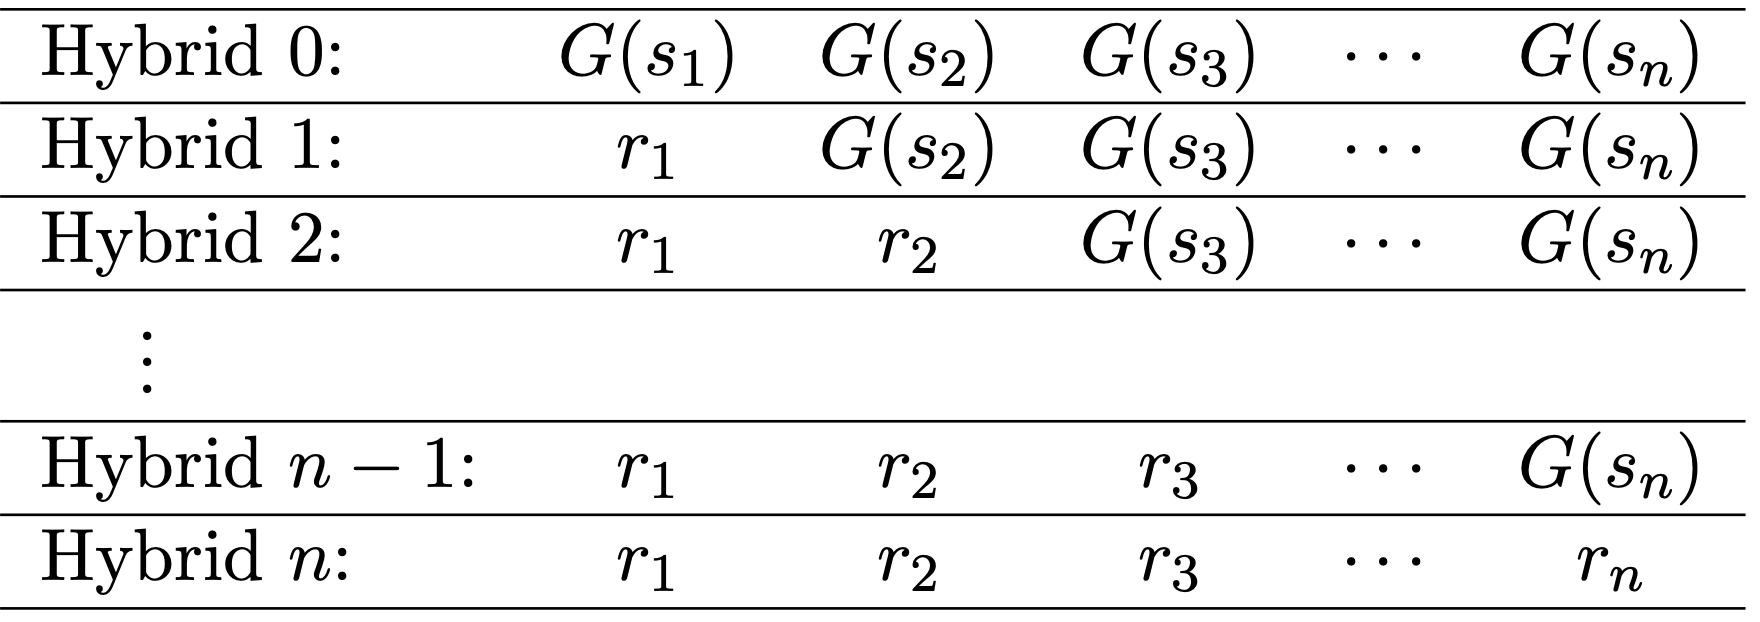
\includegraphics[width=0.55\linewidth]{figures/chapter3/fig5.png}
  \caption{挑战者在混合$0,1,\dots,n$中准备的数值。每个$r_i$都是$\mathcal{R}$上的一个随机元素,每个$s_i$都是$\mathcal{S}$上的一个随机元素。}
  \label{fig:3-5}
\end{figure}

接下来我们定义一个 PRG 对手 $\mathcal B$,它对 $G$ 进行攻击游戏 \ref{game:3-1} 中的攻击,其工作方式如下:

\vspace*{5pt}

\hspace*{5pt} 当收到来自挑战者的 $r\in\mathcal R$,$\mathcal B$ 扮演 $\mathcal A$ 的挑战者的角色:\\
\hspace*{50pt} $\omega\overset{\rm R}\leftarrow\{1,\dots,n\}$\\
\hspace*{50pt} $r_1\overset{\rm R}\leftarrow\mathcal R$\\
\hspace*{74pt} $\vdots$\\
\hspace*{50pt} $r_{\omega-1}\overset{\rm R}\leftarrow\mathcal R$\\
\hspace*{50pt} $r_{\omega}\leftarrow r$\\
\hspace*{50pt} $s_{\omega+1}\overset{\rm R}\leftarrow\mathcal{S},\;r_{\omega+1}\leftarrow G(s_{\omega+1})$\\
\hspace*{74pt} $\vdots$\\
\hspace*{50pt} $s_{n}\overset{\rm R}\leftarrow\mathcal{S},\;r_{n}\leftarrow G(s_{j+1})$\\
\hspace*{50pt} 将 $(r_1,\dots,r_n)$ 发送给 $\mathcal A$。\\
\hspace*{26pt} 最后,$\mathcal B$ 输出 $\mathcal A$ 所输出的任何东西。

\vspace*{5pt}

令 $W_0$ 是$\mathcal B$ 在攻击游戏 \ref{game:3-1} 的实验 $0$ 中输出 $1$ 的事件,$W_1$ 是$\mathcal B$在攻击游戏 \ref{game:3-1} 的实验 $1$ 中输出 $1$ 的事件。一个关键的观察是:

\begin{quote}
\emph{对于每个固定的 $j=1,\dots,n$,以 $\omega=j$ 为条件,$\mathcal B$ 的攻击游戏的实验 $0$ 就相当于混合 $j-1$,而 $\mathcal B$ 的攻击游戏的实验 $1$ 则相当于混合 $j$。
}
\end{quote}
因此:
$$
\Pr[W_0\,|\,\omega=j]=p_{j-1},\quad
\Pr[W_1\,|\,\omega=j]=p_{j}
$$
所以,我们有:
$$
\Pr[W_0]
=\sum_{j=1}^n\Pr[W_0\,|\,\omega=j]\Pr[\omega=j]
=\frac{1}{n}\sum_{j=1}^n\Pr[W_0\,|\,\omega=j]
=\frac{1}{n}\sum_{j=1}^np_{j-1}
$$
类似地:
$$
\Pr[W_1]
=\sum_{j=1}^n\Pr[W_1\,|\,\omega=j]\Pr[\omega=j]
=\frac{1}{n}\sum_{j=1}^n\Pr[W_1\,|\,\omega=j]
=\frac{1}{n}\sum_{j=1}^np_{j}
$$
最终,我们有:
$$
\begin{aligned}
{\rm PRG\mathsf{adv}}[\mathcal{B},G]
&=|\Pr[W_1]-\Pr[W_0]|\\
&=\Bigg\lvert\frac{1}{n}\sum_{j=1}^np_j-\frac{1}{n}\sum_{j=1}^np_{j-1}\Bigg\rvert\\
&=\frac{1}{n}|p_n-p_0|
\end{aligned}
$$
将其与式 \ref{eq:3-9} 相结合,我们可以得到:
$$
{\rm PRG\mathsf{adv}}[\mathcal{A},G']=n\cdot{\rm PRG\mathsf{adv}}[\mathcal{B},G]
$$
由于我们假设 $G$ 是一个安全 PRG,因此 ${\rm PRG\mathsf{adv}}[\mathcal{B},G]$ 可以忽略不计,而由于 $n$ 是多项式边界的,${\rm PRG\mathsf{adv}}[\mathcal{B},G']$ 也是可忽略不计的(见事实 \ref{fact:2-6})。这就证明了该定理。
\end{proof}

定理 3.2 表明,PRG 的安全性随着我们使用它的次数增多而最多呈线性下降。有人可能会问,这个约束是否是严格的?也即,安全性是否真的会随着使用次数的增加而线性下降?答案其实是肯定的(见练习 3.14)。

\subsection{一种串行构造:Blum-Micali 方法}\label{subsec:3-4-2}

我们下面介绍一种由 Blum 和 Micali 发明的串行构造,它使用一个只稍做延展的 PRG,建立一个可以伸展到任意长度的 PRG。

令 $G$ 是一个定义在 $(\mathcal{S},\mathcal{R}\times\mathcal{S})$ 上的 PRG,其中 $\mathcal S$ 和 $\mathcal R$ 是有限集。对于每个多项式边界的值 $n\geq 1$,我们可以构造一个定义在 $(\mathcal{S},\mathcal{R}^n\times\mathcal{S})$ 上的新的 PRG $G'$。对于 $s\in\mathcal{S}$,我们令:

\vspace*{5pt}

\hspace*{5pt} $G'(s):=$\\
\hspace*{50pt} $s_0\leftarrow s$\\
\hspace*{50pt} 对于 $i\leftarrow1$ 到 $n$:\\
\hspace*{75pt} $(r_i,s_i)\leftarrow G(s_{i-1})$\\
\hspace*{50pt} 输出$(r_1,\dots,r_n,s_n)$

\vspace*{5pt}

\noindent
我们称 $G'$ 为 $G$ 的 \textbf{$n$ 次串行组合 ($n$-wise sequential composition)}。图 \ref{fig:3-6} 是 $n=3$ 时$G'$ 的示意图。

\begin{figure}
  \centering
  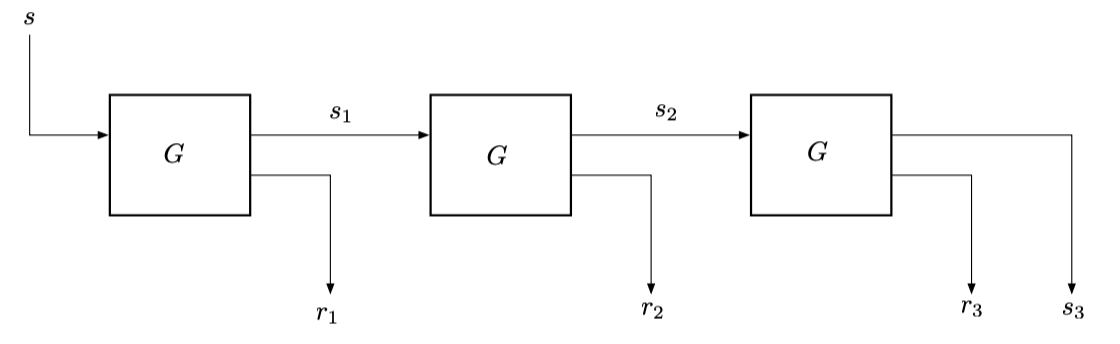
\includegraphics[width=0.8\linewidth]{figures/chapter3/fig6.png}
  \caption{$n=3$时的串行构造}
  \label{fig:3-6}
\end{figure}

我们将在下面的定理 \ref{theo:3-3} 中证明,如果 $G$ 是一个安全 PRG,那么 $G'$ 也是一个安全 PRG。作为这个构造的一个特例,假设 $G$ 是一个定义在 $(\{0,1\}^\ell,\{0,1\}^{t+\ell})$ 上的 PRG,其中 $\ell$ 和 $t$ 是正整数;也就是说,$G$ 把 $\ell$ 比特字符串拉伸为 $t+\ell$ 比特字符串。我们可以很自然地把 $G$ 的输出空间看作是 $\{0,1\}^t\times\{0,1\}^\ell$。应用上述构造,并把输出解释为比特串,我们就能得到一个PRG $G'$,它能把 $\ell$ 位比特串拉伸为 $nt+\ell$ 位比特串。

\begin{theorem}\label{theo:3-3}
如果 $G$ 是一个安全 PRG,那么 $G$ 的 $n$ 次串行组合 $G'$ 也是一个安全 PRG。
\begin{quote}
特别地,对于每个就 $G'$ 进行攻击游戏 \ref{game:3-1} 的 PRG 对手 $\mathcal A$,都存在一个就 $G$ 进行攻击游戏 \ref{game:3-1} 的 PRG 对手 $\mathcal B$,其中 $\mathcal B$ 是围绕 $\mathcal A$ 的一个基本包装器,满足:
\end{quote}
$$
{\rm PRG\mathsf{adv}}[\mathcal{A},G']=n\cdot{\rm PRG\mathsf{adv}}[\mathcal{B},G]
$$
\end{theorem}

\begin{proof}[证明思路]
该定理的证明是一个混合论证,其思路与定理 \ref{theo:3-2} 的证明非常相似。该证明背后的直觉如下所述。考虑一个 PRG 对手 $\mathcal A$,他在攻击游戏 \ref{game:3-1} 的实验 $0$ 中收到 $(r_1,\dots,r_n,s_n)$。由于 $s=s_0$ 是随机的,而且 $G$ 是一个安全 PRG,我们可以用 $\mathcal{R}\times\mathcal{S}$ 中的一个完全随机的元素来代替 $(r_1,s_1)$,且 $\mathcal A$ 在这个新的混合游戏中输出 $1$ 的概率应该只会发生可忽略不计的变化。现在,由于 $s_1$ 是随机的(同样是因为$G$ 是一个安全 PRG),我们就可以用 $\mathcal{R}\times\mathcal{S}$ 上的一个完全随机的元素来代替 $(r_2,s_2)$,而 $\mathcal A$ 在这第二个混合游戏中输出 $1$ 的概率应该也只会发生可忽略不计的变化。继续这样下去,我们可以用 $\mathcal{R}\times\mathcal{S}$ 中的随机元素逐步替换 $(r_3,s_3)$ 到 $(r_n,s_n)$,在做出这些改变之后,$\mathcal A$ 输出 $1$ 的概率应该都只会发生可忽略不计的变化(假设$n$是多项式边界的)。然而,在这一点上,$\mathcal A$ 输出 $1$ 的概率与他在攻击游戏 \ref{game:3-1} 的实验 $1$ 中输出 $1$ 的概率相同,因此,这个概率与$\mathcal A$在攻击游戏 \ref{game:3-1} 的实验 $0$ 中输出 $1$ 的概率接近得可以忽略不计。

这就是我们的想法;然而,就像在定理 \ref{theo:3-2} 的证明中一样,由于技术原因,我们设计了一个攻击$G$的 PRG 对手。
\end{proof}

\begin{proof}
令 $\mathcal A$ 是一个对 $G'$ 进行攻击游戏 \ref{game:3-1} 中的攻击的 PRG 对手。我们首先引入一个大小为 $n+1$ 的混合游戏序列,称为混合$0$,混合$1$,$\dots$,混合$n$。对于$j=0,1,\dots,n$,我们定义混合 $j$ 为 $\mathcal A$ 和以下挑战者之间的游戏。挑战者的工作方式如下:

\vspace*{5pt}

\hspace*{5pt} $r_1\overset{\rm R}\leftarrow\mathcal R$\\
\hspace*{50pt} $\vdots$\\
\hspace*{26pt} $r_j\overset{\rm R}\leftarrow\mathcal R$\\
\hspace*{26pt} $s_j\overset{\rm R}\leftarrow\mathcal S$\\
\hspace*{26pt} $(r_{j+1},s_{j+1})\leftarrow G(s_{j})$\\
\hspace*{50pt} $\vdots$\\
\hspace*{26pt} $(r_n,s_{n})\leftarrow G(s_{n-1})$\\
\hspace*{26pt} 将 $(r_1,\dots,r_n,s_n)$ 发送给 $\mathcal A$。

\vspace*{5pt}

\noindent
像之前一样,$\mathcal A$ 在游戏结束时输出 $0$ 或 $1$。图 \ref{fig:3-7} 展示了挑战者在 $n=3$ 的情况下的工作流程。请注意,$p_0$ 也等于 $\mathcal A$ 在攻击游戏 \ref{game:3-1} 的实验 $0$ 中输出 $1$ 的概率,而 $p_n$ 则等于 $\mathcal A$ 在攻击游戏 \ref{game:3-1} 的实验 $1$ 中输出 $1$ 的概率。因此,我们有:
\begin{equation}
{\rm PRG\mathsf{adv}}[\mathcal{A},G']=|p_n-p_0|
\end{equation}

接下来我们定义一个 PRG 对手 $\mathcal B$,它对 $G$ 进行攻击游戏 \ref{game:3-1} 中的攻击,其工作方式如下:

\vspace*{5pt}

\hspace*{5pt} 当收到来自挑战者的 $(r,s)\in\mathcal{R}\times\mathcal{S}$,$\mathcal B$ 扮演 $\mathcal A$ 的挑战者的角色:\\
\hspace*{50pt} $\omega\overset{\rm R}\leftarrow\{1,\dots,n\}$\\
\hspace*{50pt} $r_1\overset{\rm R}\leftarrow\mathcal R,\dots,r_{\omega-1}\overset{\rm R}\leftarrow\mathcal R$\\
\hspace*{50pt} $(r_{\omega},s_{\omega})\leftarrow(r,s)$\\
\hspace*{50pt} $(r_{\omega+1},s_{\omega+1})\leftarrow G(s_{\omega}),\dots,(r_n,s_n)\leftarrow G(s_{n-1})$\\
\hspace*{50pt} 将 $(r_1,\dots,r_n,s_n)$ 发送给 $\mathcal A$。\\
\hspace*{26pt} 最后,$\mathcal B$ 输出 $\mathcal A$ 所输出的任何东西。

\vspace*{5pt}

令 $W_0$ 是$\mathcal B$在攻击游戏 \ref{game:3-1} 的实验 $0$ 中输出 $1$ 的事件,$W_1$ 是$\mathcal B$在攻击游戏 \ref{game:3-1} 的实验 $1$ 中输出 $1$ 的事件。一个关键的观察是:
\begin{quote}
\emph{对于每个固定的 $j=1,\dots,n$,以 $\omega=j$ 为条件,$\mathcal B$ 的攻击游戏的实验 $0$ 等同于混合 $j-1$,而 $\mathcal B$ 的攻击游戏的实验 $1$ 则等同于混合 $j$。
}
\end{quote}
因此:
$$
\Pr[W_0\,|\,\omega=j]=p_{j-1},\quad
\Pr[W_1\,|\,\omega=j]=p_{j}
$$

\begin{figure}
  \centering
  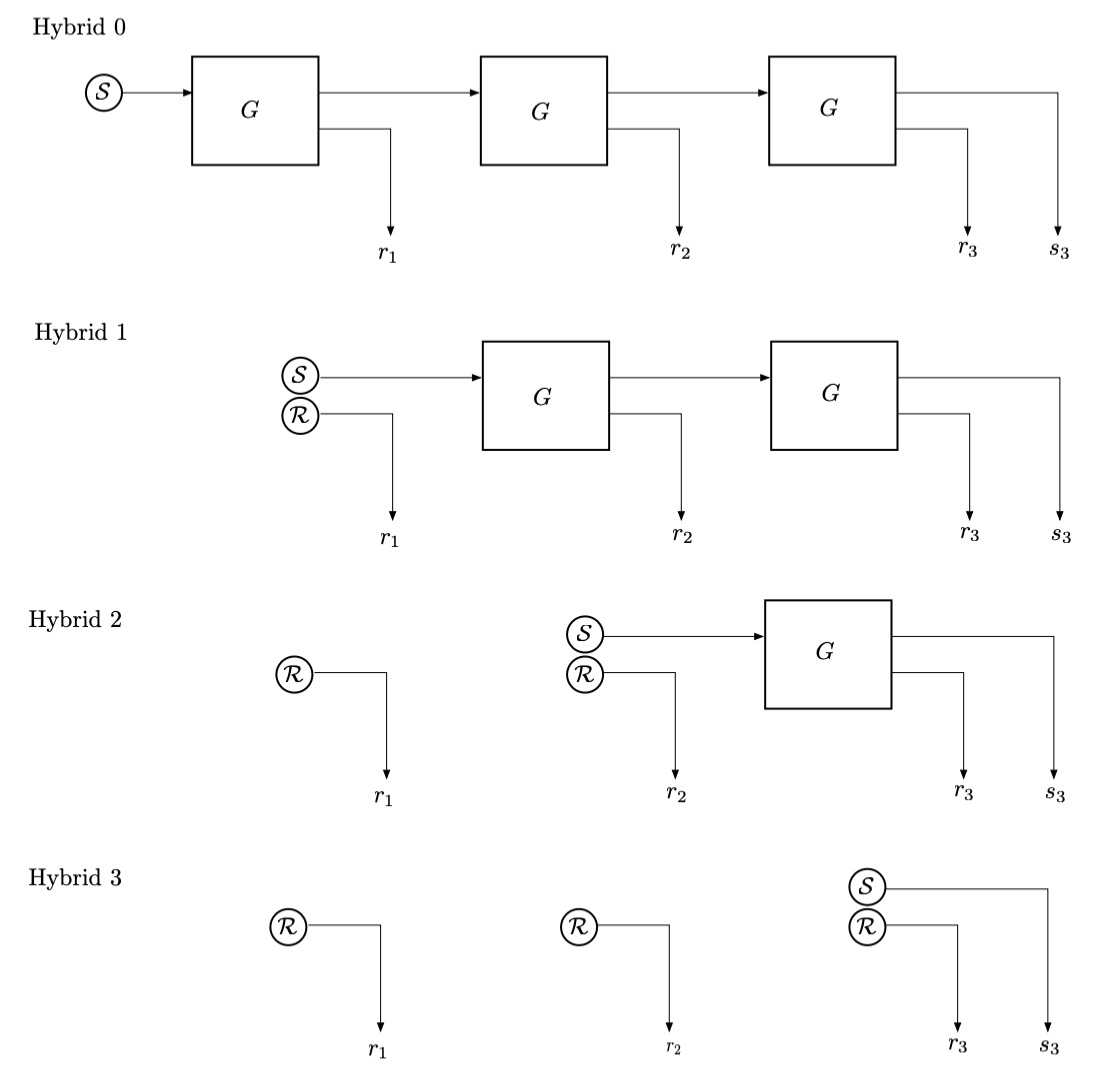
\includegraphics[width=0.8\linewidth]{figures/chapter3/fig7.png}
  \caption{$n=3$时,混合游戏中挑战者的计算。圆圈表示随机产生的$\mathcal{S}$或$\mathcal{R}$上的元素,如标签所示。}
  \label{fig:3-7}
\end{figure}

接下来的证明只是简单的计算,与定理 \ref{theo:3-2} 的证明的最后一段\emph{相同},不再赘述。
\end{proof}

评价 PRG 的一个标准是它的\textbf{扩展率 (expansion rate)}:一个将 $n$ 比特种子扩展到 $m$ 比特输出的 PRG 的扩展率为 ${m}/{n}$。更一般地说,如果种子空间是 $\mathcal{S}$,输出空间是 $\mathcal{\rm R}$,我们将扩展率定义为 ${\log|\mathcal{\rm R}|}/{\log|\mathcal{S}|}$。串行组合构造比并行组合构造提供了更好的扩展率,但是它有一个缺点,那就是它不能被并行化。事实上,存在一种构造可以兼顾两种优点:大的扩展率和高度可并行的结构,见 \ref{subsec:4-4-4} 小节。

\subsection{数学细节}

在定理 \ref{theo:3-2} 和 \ref{theo:3-3} 的证明中,有一些微妙的地方值得讨论。

首先,在这两个构造中,底层的 PRG $G$ 可能有系统参数。也就是说,可能存在一个概率性算法,它将安全参数 $\lambda$ 作为输入,并输出一个系统参数 $\Lambda$。回顾一下,系统参数是能够完全将构造实例化的公共数据(在这个场景中,它可能定义了种子空间和输出空间)。对于并行和串行构造,我们可以对 $G$ 的所有 $n$ 个实例使用相同的系统参数;事实上,对于串行构造来说,这是必须的,因为我们要确保一轮的输出可以被用作下一轮的输入。无论是对所有 $G$ 的实例使用相同的系统参数,还是对不同的实例使用不同的系统参数,这些安全定理的证明都是完全有效的。

其次,我们要简要讨论关于混合论证的一个相当深奥的问题。为了更具体一点,我们把注意力集中在定理 \ref{theo:3-2} 的证明上(尽管类似的讨论也适用于定理 \ref{theo:3-3} 的证明,或任何其他的混合论证)。在证明该定理时,我们最终想要证明,如果存在一个能破解 $G'$ 的有效对手 $\mathcal A$,那么也必然存在一个能破解 $G$ 的有效对手。假设 $\mathcal A$ 是一个能破解 $G'$ 的有效对手,那么它相对于 $G'$ 的优势 $\epsilon(\lambda)$(我们这里明确地把它表示成安全参数$\lambda$的一个函数)是不可忽略不计的。这意味着存在一个常数 $c$使得 $\epsilon(\lambda)\geq{1}/{\lambda^c}$适用于无限多的 $\lambda$。

现在,在定理 \ref{theo:3-2} 证明之前的讨论中,我们考虑了 $n=2$ 的特殊情况,并表明存在有效对手 $\mathcal{B}_1$ 和 $\mathcal{B}_2$,使得 $\epsilon(\lambda)\leq\delta_1(\lambda)+\delta_2(\lambda)$ 对于任意 $\lambda$ 都成立,其中 $\delta_j(\lambda)$ 表示 $\mathcal{B}_j$ 相对于 $G$ 的优势。由此可见,要么 $\delta_1(\lambda)\geq{1}/{2\lambda^c}$ 无限频繁,要么 $\delta_2(\lambda)\geq{1}/{2\lambda^c}$ 无限频繁。因此我们可以得出结论,要么是$\mathcal{B}_1$ 打破 $G$,要么是$\mathcal{B}_2$ 打破 $G$(也可能两者皆然)。因此,\emph{存在}一个能破解 $G$ 的有效对手:它要么是 $\mathcal{B}_1$ 要么是 $\mathcal{B}_2$,我们不知道到底是哪一个(也不必分清是哪一个)。然而无论是哪一个,它都是一个固定的对手,对所有的 $\lambda$ 都是统一定义的;也就是说,它是一个固定的,以 $\lambda$ 为输入的机器。

这个论证是完全有效的,并且可以扩展到任意\emph{常数} $n$:我们可以构造 $n$ 个对手 $\mathcal{B}_1,\dots,\mathcal{B}_n$,并论证对于某个 $j\in\{1,\dots,n\}$,对手 $\mathcal{B}_j$ 无限频繁地对 $G$ 有优势 ${1}/{n\lambda^c}$,从而攻破 $G$。然而这个论证并没有扩展到 $n$ 是 $\lambda$ 的函数的情况,我们现在把它明确写成 $n(\lambda)$。问题不在于 ${1}/({n(\lambda)\lambda^c})$ 也许太小(其实并不是)。这个问题相当微妙,所以在我们讨论它之前,让我们先回顾一下我们所给出的(合法)证明。对于每个 $\lambda$,我们定义一个大小为 $n(\lambda)+1$ 的混合游戏序列,因此对于每个 $\lambda$,我们实际上得到了一个不同的游戏序列。事实上,我们不能说有一个单一、有限的游戏序列对所有 $\lambda$ 都有效,因为 $n(\lambda)\to\infty$。尽管如此,我们还是明确地构造了一个固定的对手 $\mathcal B$,它是为所有 $\lambda$ 统一定义的;也就是说,$\mathcal B$ 是一个固定的机器,它把 $\lambda$ 作为输入。我们为每个 $\lambda$ 定义的混合游戏序列是一个数学对象,我们对其可计算性不做任何主张,它只是在分析 $\mathcal B$ 时使用的一个方便的工具。

希望到现在为止,读者至少对我们试图将常数 $n$ 的论证推广到一个函数 $n(\lambda)$ 时所产生的问题有了一个直观感觉。首先,我们甚至不清楚 $n(\lambda)$ 个对手 $\mathcal{B}_1,\dots,\mathcal{B}_{n(\lambda)}$ 是什么意思:我们的对手应该是将 $\lambda$ 作为输入的固定机器,而机器本身不应该依赖于 $\lambda$。撇开这种语言上的混乱不谈,我们对常数情况的证明只表明存在一个``对手",对于无限多的 $\lambda$ 值来说,它能以某种方式知道 $j=j(\lambda)$ 的``正确"值,以便在 $(n(\lambda)+1)$ 游戏混合论证中使用——没有一个 $j$ 常数值一定对无限多的 $\lambda$ 有效。如果使用非统一的计算模型,我们实际上可以使这种类型的论证有意义,但我们在本文中不会采取这种方法。

当我们使用一个构建单一对手 $\mathcal B$ 的混合论证时,所有这些问题都会消失,就像我们在定理 \ref{theo:3-2} 和 \ref{theo:3-3} 的证明中所做的。然而我们重申,我们在 $n=2$,或自然延伸到每一个常数 $n$ 的情况下所做的原始分析是完全有效的。在这种情况下,我们构建了一个单一、固定的 $n+1$ 游戏序列,每个单独的游戏对所有 $\lambda$ 都是统一定义的(就像我们的安全定义中的攻击游戏一样),我们还定义了一个有限的对手集合,每个对手都是一个固定的机器。我们重申这一点,因为在后面的内容中,我们将经常构建涉及这样的有限序列游戏的证明(事实上,定理\ref{theo:3-1}的证明就是这种类型)。在这种情况下,每个游戏将为所有 $\lambda$ 统一定义,并被称为游戏 $0$、游戏 $1$,等等。相反,当我们进行混合论证,使用非均匀的游戏序列时,我们将这些游戏表示为混合 $0$,混合 $1$ 等,以避免任何可能的混淆。
\section{下一比特测试}

令 $G$ 是一个定义在 $(\{0,1\}^\ell,\{0,1\}^L)$ 上的 PRG,它能将 $\ell$ 比特字符串拉伸到 $L$ 比特长。有许多方法可以让对手区分 $G$ 的伪随机输出和真正的随机比特序列。事实上,假设一个有效对手能在给定 $G$ 输出的前 $L-1$ 比特的情况下预测出其输出的最后一比特,则 $G$ 从直观上来说就是不安全的,因为给定一个真随机 $L$ 位比特序列的前 $L-1$ 位,任何人最多只有一半的机会猜中最后一比特。事实上,该结论一个有趣的逆命题也是真命题。

我们下面会正式定义 PRG 的\textbf{不可预测性 (unpredictability)} 的概念。它本质上指,给定 $G$ 输出的前 $i$ 比特(这里的$i$是一个对手选择的索引),能够以显著高于$1/2$的概率预测出下一个比特(即第 $i+1$ 比特)是困难的。之后,我们将证明不可预测性和安全性是等价的。安全性能够导出不可预测性这一事实是很直观的:如果能够有效预测伪随机序列中的下一比特,那么我们就能直接给出一个有效的统计测试来打破安全性。相反,由不可预测性能够导出安全性,这是相当有趣的(需要花一些精力来证明),这实际上是指,如果存在任何有效的统计测试能够打破 PRG 的安全性,那么必然存在一个方法能够有效预测伪随机序列将要输出的下一比特。

\begin{game}[不可预测的 PRG]\label{game:3-2}
对于一个定义在 $(\mathcal{S},\{0,1\}^L)$ 上的给定 PRG $G$ 和一个给定对手 $\mathcal{A}$,攻击游戏的过程如下:
\begin{itemize}
	\item 对手向挑战者发送一个索引 $i$,其中 $0\leq i\leq L-1$。
	\item 挑战者计算
	$$s\overset{\rm R}\leftarrow\mathcal{S},\;\; r\leftarrow G(s)$$
	并将 $r[0\dots i-1]$ 发送给对手。
	\item 对手输出 $g\in\{0,1\}$。
\end{itemize}
如果 $r[i]=g$,我们就说 $\mathcal{A}$ \textbf{获胜}。我们定义 $\mathcal{A}$ 相对于 $G$ 的\textbf{优势}为 ${\rm Pred\mathsf{adv}}[\mathcal{A},G]$,其值为$|\Pr[\mathcal{A}\text{ wins}]-{1}/{2}|$。
\end{game}

\begin{definition}[不可预测的 PRG]
如果 ${\rm Pred\mathsf{adv}}[\mathcal{A},G]$ 对所有有效对手 $\mathcal{A}$ 来说都是可忽略不计的,那么 PRG $G$ 就是\textbf{不可预测的 (unpredictable)}。
\end{definition}

我们下面先证明安全性能够推出不可预测性。

\begin{theorem}
令 $G$ 是一个定义在 $(\mathcal{S},\{0,1\}^L)$ 上的 PRG。如果 $G$ 是安全的,那么 $G$ 就是不可预测的。
\begin{quote}
特别地,对于每个如攻击游戏 \ref{game:3-2} 那样攻击 $G$ 的不可预测性对手 $\mathcal{A}$,必然存在一个如攻击游戏 \ref{game:3-1} 那样攻击 $G$ 的安全性对手 $\mathcal{B}$,其中 $\mathcal{B}$ 是围绕 $\mathcal{A}$ 的一个基本包装器,满足:
\end{quote}
$$
{\rm Pred\mathsf{adv}}[\mathcal{A},G]={\rm PRG\mathsf{adv}}[\mathcal{B},G]
$$
\end{theorem}

\begin{proof}
令 $\mathcal{A}$ 是一个攻击 $G$ 的不可预测性的对手,令 $i$ 表示 $\mathcal{A}$ 所选择的索引。同时,假设 $\mathcal{A}$ 能以 ${1}/{2}+\epsilon$ 的概率赢得攻击游戏 \ref{game:3-2},则有${\rm Pred\mathsf{adv}}[\mathcal{A},G]=|\epsilon|$。

我们下面以 $\mathcal{A}$ 为子程序,建立一个攻击 $G$ 的安全性的对手 $\mathcal{B}$,其运行方式如下:

\vspace*{5pt}

\hspace*{5pt} 当收到来自挑战者的 $r\in\{0,1\}^L$ 时,$\mathcal B$ 进行以下操作:\\
\hspace*{50pt} $\mathcal{B}$ 将 $r[0\dots i-1]$ 发送 $\mathcal{A}$,获得 $\mathcal{A}$ 的输出 $g\in\{0,1\}$;\\
\hspace*{50pt} 如果 $r[i]=g$,$\mathcal{B}$ 输出 $1$,否则输出 $0$。

\vspace*{5pt}

对于 $b=0,1$,令 $W_b$ 为$\mathcal{B}$在攻击游戏 \ref{game:3-1} 的实验 $b$ 中输出 $1$ 的事件。在实验 $0$ 中,$r$ 是 $G$ 的一个伪随机输出,当且仅当 $r[i]=g$ 时 $W_0$ 才会发生,因此根据定义,有:
$$
\Pr[W_0]={1}/{2}+\epsilon
$$
在实验 $1$ 中,$r$ 是一个真随机比特序列。同样地,当且仅当 $r[i]=g$ 时 $W_1$ 才会发生;然而,在这种情况下,随机变量 $r[i]$ 和 $g$ 的值相互独立,因此有:
$$
\Pr[W_1]={1}/{2}
$$
因此可以得到:
$$
{\rm Pred\mathsf{adv}}[\mathcal{B},G]=|\Pr[W_1]-\Pr[W_0]|=|\epsilon|={\rm PRG\mathsf{adv}}[\mathcal{A},G]
$$
\end{proof}

更有趣也更有挑战性的任务是证明不可预测性能够推出着安全性。在详细介绍具体的证明之前,我们先勾勒出高层次的想法。

首先,我们会采用一个混合论证,目的是论证如果 $\mathcal{A}$ 是一个能够有效区分伪随机 $L$ 比特序列和真随机 $L$ 比特序列的有效对手,那么我们必然可以构造一个有效对手 $\mathcal{B}$,他能够有效地区分:
$$
x_1\cdots x_j~r
$$
和:
$$
x_1\cdots x_j~x_{j+1}
$$
其中 $j$ 是一个随机选出的索引,$x_1,\dots,x_L$ 是伪随机输出,而 $r$ 是一个随机比特。因此,对手 $\mathcal{B}$ 可以在给定 $x_1,\dots,x_j$ 这个``侧信息"的情况下有效区分伪随机比特 $x_{j+1}$ 和真随机比特 $r$。

我们想把 $\mathcal{B}$ 的区分优势变成预测优势,大致的想法是这样的:给定 $x_1,\dots,x_j$,我们给 $\mathcal{B}$ 提供一个序列 $x_1\cdots x_j~r$,其中的 $r$ 是一个随机选出的比特;如果 $\mathcal{B}$ 输出 $1$,我们对 $x_{j+1}$ 的预测值就是 $r$;否则我们对 $x_{j+1}$ 的预测值就是 $\overline r$($r$ 的补码)。

这一预测策略的有效性由以下的一般结论给出,我们称之为\emph{区分者/预测者引理}。我们有一半设置如下:
\begin{itemize}
	\item 一个随机变量 $\mathsf{X}$,它对应于上面的``侧信息" $x_1,\dots,x_j$ 以及对手 $\mathcal{B}$ 所使用的任何随机硬币;
	\item 一个取值为 $0$ 或 $1$ 的随机变量 $\mathsf{B}$,它对应于上面的 $x_{j+1}$,并可能与 $\mathsf{X}$ 相关;
	\item 一个取值为 $0$ 或 $1$ 的随机变量 $\mathsf{R}$,它对应于上面的 $r$,并且与 $(\mathsf{X},\mathsf{B})$ 无关。
	\item 一个函数 $d$,它对应于使得$\mathcal{B}$的区分优势为$|\epsilon|$的策略,其中$\epsilon=\Pr[d(\mathsf{X},\mathsf{B})=1]-\Pr[d(\mathsf{X},\mathsf{R})=1]$。
\end{itemize}
该引理表明,如果我们用上述预测策略定义 $\mathsf{B}'$,即如果 $d(\mathsf{X},\mathsf{R})=1$,就有 $\mathsf{B}'=\mathsf{R}$,否则有 $\mathsf{B}'=\mathsf{\overline R}$,那么预测 $\mathsf{B}'$ 等于实际值 $\mathsf{B}$ 的概率正好是 ${1}/{2}+\epsilon$。下面是该引理的精确陈述:

\begin{lemma}[区分者/预测者引理]\label{lemma:3-5}
令 $\mathsf{X}$ 是一个在某个集合 $S$ 中取值的随机变量,令 $\mathsf{B}$ 和 $\mathsf{R}$ 是取值为 $0$ 或 $1$ 的随机变量,其中 $\mathsf{R}$ 在 $\{0,1\}$ 上均匀分布,且与 $(\mathsf{X},\mathsf{B})$ 无关。令 $d:S\times\{0,1\}\to\{0,1\}$ 是一个任意的函数,并令:
$$
\epsilon:=\Pr[d(\mathsf{X},\mathsf{B})=1]-\Pr[d(\mathsf{X},\mathsf{R})=1]
$$
随机变量 $\mathsf{B}'$的定义如下:
$$
\mathsf{B}':=
\left\{
\begin{array}{ll}
\mathsf{R}, & d(\mathsf{X},\mathsf{R})=1\\
\mathsf{\overline R}, & d(\mathsf{X},\mathsf{R})\neq 1
\end{array}
\right.
$$
则有:
$$
\Pr[\mathsf{B}'=\mathsf{B}]={1}/{2}+\epsilon
$$
\end{lemma}

\begin{proof}
我们首先以事件 $\mathsf{B}=\mathsf{R}$ 和 $\mathsf{B}=\mathsf{\overline R}$ 为条件计算 $\Pr[\mathsf{B}'=\mathsf{B}]$:

$$
\begin{aligned}
\Pr[\mathsf{B}'=\mathsf{B}]
&=\Pr[\mathsf{B}'=\mathsf{B}\,|\,\mathsf{B}=\mathsf{R}]\cdot\Pr[\mathsf{B}=\mathsf{R}]+\Pr[\mathsf{B}'=\mathsf{B}\,|\,\mathsf{B}=\mathsf{\overline R}]\cdot\Pr[\mathsf{B}=\mathsf{\overline R}]\\
&=\Pr[d(\mathsf{X},\mathsf{R})=1\,|\,\mathsf{B}=\mathsf{R}]\cdot\frac{1}{2}+\Pr[d(\mathsf{X},\mathsf{R})=0\,|\,\mathsf{B}=\mathsf{\overline R}]\cdot\frac{1}{2}\\
&=\frac{1}{2}
\Big(\Pr[d(\mathsf{X},\mathsf{R})=1\,|\,\mathsf{B}=\mathsf{R}]+
\big(
1-\Pr[d(\mathsf{X},\mathsf{R})=1\,|\,\mathsf{B}=\mathsf{\overline R}]
\big)
\Big)\\
&=\frac{1}{2}+\frac{1}{2}(\alpha-\beta)
\end{aligned}
$$
其中:
$$
\alpha:=\Pr[d(\mathsf{X},\mathsf{R})=1\,|\,\mathsf{B}=\mathsf{R}],\quad
\beta:=\Pr[d(\mathsf{X},\mathsf{R})=1\,|\,\mathsf{B}=\mathsf{\overline R}]
$$
根据独立性,我们有:
$$
\alpha=\Pr[d(\mathsf{X},\mathsf{R})=1\,|\,\mathsf{B}=\mathsf{R}]=\Pr[d(\mathsf{X},\mathsf{B})=1\,|\,\mathsf{B}=\mathsf{R}]=\Pr[d(\mathsf{X},\mathsf{B})=1]
$$
想要知道最后一个等式为什么成立,可以参考练习 3.25 的结论。

因此,我们可以计算出:
$$
\begin{aligned}
\epsilon
&=\Pr[d(\mathsf{X},\mathsf{B})=1]-\Pr[d(\mathsf{X},\mathsf{R})=1]\\
&=\alpha-
\Big(\Pr[d(\mathsf{X},\mathsf{R})=1\,|\,\mathsf{B}=\mathsf{R}]\cdot\Pr[\mathsf{B}=\mathsf{R}]+\Pr[d(\mathsf{X},\mathsf{R})=1\,|\,\mathsf{B}=\mathsf{\overline R}]\cdot\Pr[\mathsf{B}=\mathsf{\overline R}]
\Big)\\
&=\alpha-\frac{1}{2}(\alpha+\beta)\\
&=\frac{1}{2}(\alpha-\beta)
\end{aligned}
$$
这就证明了该引理。
\end{proof}

\begin{theorem}
令 $G$ 是一个定义在 $(\mathcal{S},\{0,1\}^L)$ 上的 PRG。如果 $G$ 是不可预测的,那么 $G$ 就是安全的。
\begin{quote}
特别地,对于每个像攻击游戏 \ref{game:3-1} 那样攻击 $G$ 的安全性的对手 $\mathcal{A}$,必然存在一个像攻击游戏 \ref{game:3-2} 那样攻击 $G$ 的不可预测性的对手 $\mathcal{B}$,其中 $\mathcal{B}$ 是围绕 $\mathcal{A}$ 的一个基本包装器,满足:
\end{quote}
$$
{\rm PRG\mathsf{adv}}[\mathcal{A},G]=L\cdot{\rm Pred\mathsf{adv}}[\mathcal{B},G]
$$
\end{theorem}

\begin{proof}
令 $\mathcal{A}$ 像攻击游戏 \ref{game:3-1} 中那样攻击 $G$。利用 $\mathcal{A}$,我们建立一个预测器 $\mathcal{B}$,它像攻击游戏 \ref{game:3-2} 那样攻击 $G$。$\mathcal{B}$ 的工作方式如下:
\begin{itemize}
	\item 随机选出 $\omega\in\{1,\dots,L\}$。
	\item 向挑战者发送 $L-\omega$,得到一个字符串 $x\in\{0,1\}^{L-\omega}$。
	\item 随机生成 $\omega$ 个比特 $r_1,\dots,r_\omega$,并将 $L$ 比特序列 $x~||~r_1\cdots r_\omega$ 发送给 $\mathcal{A}$。
	\item 如果 $\mathcal{A}$ 输出 $1$,则 $\mathcal{B}$ 输出 $r_1$,否则 $\mathcal{B}$ 输出 $\overline r_1$。
\end{itemize}

为了分析 $\mathcal{B}$,我们考虑 $L+1$ 个混合游戏,称为混合$0$,混合$1$,$\dots$,混合$L$。对于 $j=0,\dots,L$,我们定义混合 $j$ 为 $\mathcal{A}$ 和挑战者之间的游戏,挑战者生成一个由 $L-j$ 个伪随机比特和 $j$ 个真随机比特组成的序列 $r$;也就是说,挑战者随机选择 $s\in\mathcal{S}$ 和 $t\in\{0,1\}^j$,并向 $\mathcal{A}$ 发送比特序列:
$$
r=G(s)[0\dots L-j-1]~||~t
$$
和之前一样,$\mathcal{A}$ 在游戏结束时输出 $0$ 或 $1$,我们定义 $p_j$ 为 $\mathcal{A}$ 在混合 $j$ 中输出 $1$ 的概率。注意 $p_0$ 是 $\mathcal{A}$ 在攻击游戏 \ref{game:3-1} 的实验 $0$ 中输出 $1$ 的概率,而 $p_L$ 是 $\mathcal{A}$ 在攻击游戏 \ref{game:3-1} 的实验 $1$ 中输出 $1$ 的概率。

令 $W$ 为 $\mathcal{B}$ 在攻击游戏 \ref{game:3-2} 中获胜的事件(即他正确预测了下一个比特),那么我们有:
$$
\begin{aligned}
\Pr[W]
&=\sum_{j=1}^L\Pr[W|\omega=j]\cdot\Pr[\omega=j]\\
&=\frac{1}{L}\sum_{j=1}^L\Pr[W\,|\,\omega=j]\\
&=\frac{1}{L}\sum_{j=1}^L
\Big(\frac{1}{2}+p_{j-1}-p_j
\Big)
\quad\text{\emph{(根据引理} \ref{lemma:3-5}\emph{\,)}}\\
&=\frac{1}{2}+\frac{1}{L}(p_0-p_L)
\end{aligned}
$$
这就证明了该定理。
\end{proof}
\section{案例研究:Salsa 和 ChaCha PRG}\label{sec:3-6}

在实践中,有许多建立 PRG 和流密码的方法。一种方法是使用 \ref{subsec:3-4-2} 小节中介绍的 Blum-Micali 范式来构建 PRG。我们还将会在第\ref{chap:5}章中讨论另一种方法,它将使用一种更加通用的密码学原语(即计数器模式下的\emph{伪随机函数})来构建它们。我们从一个基于后者的构造开始。

Salsa20/12 和 Salsa20/20 是 Dan Bernstein 于 2005 年设计的快速流密码。Salsa20/12 是被选入 eStream 流密码组合的四种Profile 1 流密码之一。eStream 是一个旨在选择适用于实际场景中的快速且安全的流密码的项目。Bernstein 又于 2008 年提出了 Salsa20/12 和 Salsa20/20 的变体,分别被称作 ChaCha12 和 ChaCha20。这些流密码已经被用在了一些广泛部署的协议——比如 TLS 和 SSH——之中了。

\begin{figure}
	\centering
	\tikzset{every picture/.style={line width=0.75pt}}

\begin{tikzpicture}[x=0.75pt,y=0.75pt,yscale=-0.9,xscale=0.9]

\draw  [line width=1]  (0,0) -- (40,0) -- (40,30) -- (0,30) -- cycle ;
\draw  [line width=1.2]  (80,40) -- (200,40) -- (200,70) -- (80,70) -- cycle ;
\draw  [line width=1.2]  (240,40) -- (360,40) -- (360,70) -- (240,70) -- cycle ;
\draw  [line width=1.2]  (400,40) -- (520,40) -- (520,70) -- (400,70) -- cycle ;
\draw  [line width=1.2]  (80,240) -- (200,240) -- (200,270) -- (80,270) -- cycle ;
\draw  [line width=1.2]  (240,240) -- (360,240) -- (360,270) -- (240,270) -- cycle ;
\draw  [line width=1.2]  (400,240) -- (520,240) -- (520,270) -- (400,270) -- cycle ;

\draw  [fill={rgb, 255:red, 155; green, 155; blue, 155 }  ,fill opacity=0.5 ][line width=1.5]  (100,110) -- (180,110) -- (180,180) -- (100,180) -- cycle ;
\draw  [fill={rgb, 255:red, 155; green, 155; blue, 155 }  ,fill opacity=0.5 ][line width=1.5]  (260,110) -- (340,110) -- (340,180) -- (260,180) -- cycle ;
\draw  [fill={rgb, 255:red, 155; green, 155; blue, 155 }  ,fill opacity=0.5 ][line width=1.5]  (420,110) -- (500,110) -- (500,180) -- (420,180) -- cycle ;

\draw  [->]  (40,15) -- (460,15) -- (460,40) ;
\draw  [->]  (300,15) -- (300,40) ;
\draw  [->]  (140,15) -- (140,40) ;
\draw  [->]  (140,70) -- (140,110) ;
\draw  [->]  (300,70) -- (300,110) ;
\draw  [->]  (460,70) -- (460,110) ;
\draw  [->]  (140,180) -- (140,202) ;
\draw  [->]  (300,180) -- (300,202) ;
\draw  [->]  (460,180) -- (460,202) ;
\draw  [->]  (140,218) -- (140,240) ;
\draw  [->]  (300,218) -- (300,240) ;
\draw  [->]  (460,218) -- (460,240) ;
\draw  [->]  (140,90) -- (70,90) -- (70,210) -- (132,210) ;
\draw  [->]  (300,90) -- (230,90) -- (230,210) -- (292,210) ;
\draw  [->]  (460,90) -- (390,90) -- (390,210) -- (452,210) ;

\draw (140,145) node   {$\displaystyle\prod $};
\draw (300,145) node   {$\displaystyle\prod $};
\draw (460,145) node   {$\displaystyle\prod $};

\draw (140,55) node    {$\mathrm{pad}( \cdot ,\mathbf{0} ,\textcolor[rgb]{0.61,0.61,0.61}{0})$};
\draw (300,55) node    {$\mathrm{pad}( \cdot ,\mathbf{1} ,\textcolor[rgb]{0.61,0.61,0.61}{0})$};
\draw (460,55) node    {$\mathrm{pad}( \cdot ,\mathbf{2} ,\textcolor[rgb]{0.61,0.61,0.61}{0})$};

\draw (20,15) node  [font=\small] [align=left] {种子};
\draw (140,210) node    {$\bigoplus $};
\draw (300,210) node    {$\bigoplus $};
\draw (460,210) node    {$\bigoplus $};
\draw (140,255) node  [font=\small] [align=left] {输出分组 \#$ 0$};
\draw (300,255) node  [font=\small] [align=left] {输出分组 \#$ 1$};
\draw (460,255) node  [font=\small] [align=left] {输出分组 \#$ 2$};
\draw (180,85) node  [font=\small] [align=left] {$ 512$ 比特};
\draw (140,285) node [font=\small]  [align=left] {$ 512$ 比特};
\draw (300,285) node [font=\small]  [align=left] {$ 512$ 比特};
\draw (460,285) node [font=\small]  [align=left] {$ 512$ 比特};
\draw (560,55) node   [align=left] {$ \cdots $};
\draw (560,255) node   [align=left] {$ \cdots $};
\draw (-3,45) node [anchor=west] [inner sep=0.75pt]  [font=\small] [align=left] {$ 256$ 比特};

\end{tikzpicture}
	\caption{Salsa 和 ChaCha PRG 的示意图}
	\label{fig:3-8}
\end{figure}

让我们先简单介绍一下 Salsa 和 ChaCha 流密码家族的底层 PRG。这些 PRG 将一个 $256$ 比特的种子和一个 $64$ 比特的 nonce 作为输入。我们暂时先忽略 nonce,简单地将其置为 $0$,我们将在本节末尾讨论 nonce 的作用。Salsa 和 ChaCha PRG 都遵循图 \ref{fig:3-8} 所示的上层结构。它们都包含两个组件:
\begin{itemize}
	\item 一个填充函数 $\mathrm{pad}(s,j,0)$,它将一个 $256$ 比特的种子 $s$ 和一个 $64$ 比特的计数器 $j$ 结合,以生成一个 $512$ 比特的分组。第三个输入是一个 $64$ 比特的 nonce,我们目前先把它置为 $0$。
	\item 一个固定且公开的置换 $\pi:\{0,1\}^{512}\to\{0,1\}^{512}$。
\end{itemize}
这两个组件使用以下算法(见图 \ref{fig:3-8})输出 $L<2^{64}$ 个伪随机分组,每个 $512$ 比特长:

\vspace*{10pt}

\hspace*{5pt} 输入:种子$s\in\{0,1\}^{256}$

\vspace*{5pt}

\hspace*{5pt} 1. \quad 对于 $j\leftarrow0$ 到 $L-1$:\\
\hspace*{26pt} 2. \quad\quad\quad\quad$h_j\leftarrow\mathrm{pad}(s,j,0)\in\{0,1\}^{512}$\\
\hspace*{26pt} 3. \quad\quad\quad\quad$r_j\leftarrow\pi(h_j)\oplus h_j$\\
\hspace*{26pt} 4. \quad 输出 $(r_0,\dots,r_{L-1})$。

\vspace*{10pt}

\noindent
PRG 的最终输出有 $512\cdot L$ 比特长。我们注意到,在 Salsa 和 ChaCha 中,第 $3$ 行中的异或运算实际上是一个更加复杂的操作:将 $512$ 比特的操作数 $h_j$ 和 $\pi(h_j)$ 拆分成 $16$ 个字,每个字长 $32$ 比特,然后逐字计算模 $2^{32}$ 加法。

Salsa 和 ChaCha 的设计是高度并行的,并且可以同时利用多个处理器核心来加快加密速度。此外,它还可以实现对输出分组的随机访问:不必计算出所有的前序分组,就可以单独计算输出中编号为 $j$ 的分组。基于 Blum-Micali 范式的生成器就不具备这些特性。

我们将在下一章的练习 \ref{exer:4-23} 中分析 Salsa 和 ChaCha 的安全性,但在那之前,我们还需要其他的一些密码学工具。

\begin{snote}[实现细节。]
我们下面简单介绍 ChaCha20 中使用的填充函数 $\mathrm{pad}(s,j,n)$ 和置换 $\pi$。填充函数的输入是一个 $256$ 比特的种子$s_0,\dots,s_7\in\{0,1\}^{32}$,一个 $64$ 比特的计数器 $j_0,j_1\in\{0,1\}^{32}$,以及一个 $64$ 比特的 nonce $n_0,n_1\in\{0,1\}^{32}$。它输出一个 $512$ 比特的分组,记为 $x_0,\dots,x_{15}\in\{0,1\}^{32}$。输出会被组织为一个由 $32$ 比特字构成的 $4\times4$ 矩阵,如下所示:
\begin{equation}
\begin{pmatrix}
x_0 & x_1 & x_2 & x_3 \\
x_4 & x_5 & x_6 & x_7 \\
x_8 & x_9 & x_{10} & x_{11} \\
x_{12} & x_{13} & x_{14} & x_{15}
\end{pmatrix}
\longleftarrow
\begin{pmatrix}
c_0 & c_1 & c_2 & c_3 \\
s_0 & s_1 & s_2 & s_3 \\
s_4 & s_5 & s_6 & s_7 \\
j_0 & j_1 & n_0 & n_1
\end{pmatrix}
\end{equation}
其中 $c_0,c_1,c_2,c_3$ 都是固定的 $32$ 比特常数。

通过对一个简单的置换进行固定次数的迭代,我们就能够得到置换 $\pi:\{0,1\}^{512}\to\{0,1\}^{512}$。$\pi$ 的 $512$ 比特输入会被当作一个由 $16$ 个 $32$ 比特字 $x_0,\dots,x_{15}$ 构成的 $4\times4$ 数组。在 ChaCha20 中,函数 $\pi$ 是通过重复 $10$ 次下列步骤实现的:
\begin{center}
\begin{tabular}{ll}
 (1) $\mathrm{QuarterRound}(x_0,x_4,x_8,x_{12})$, & (2) $\mathrm{QuarterRound}(x_1,x_5,x_9,x_{13})$,\\ 
 (3) $\mathrm{QuarterRound}(x_2,x_6,x_{10},x_{14})$, & (4) $\mathrm{QuarterRound}(x_3,x_7,x_{11},x_{15})$,\\  
 (5) $\mathrm{QuarterRound}(x_0,x_5,x_{10},x_{15})$, & (6) $\mathrm{QuarterRound}(x_1,x_6,x_{11},x_{12})$,\\
 (7) $\mathrm{QuarterRound}(x_2,x_7,x_8,x_{13})$, & (8) $\mathrm{QuarterRound}(x_3,x_4,x_9,x_{14})$\\
\end{tabular}
\end{center}
这里,$\mathrm{QuarterRound}(\texttt{a},\texttt{b},\texttt{c},\texttt{d})$ 的定义可参见下面用 C 程序表示的步骤:
\begin{center}
\begin{tabular}{lll}
\texttt{a += b;} & \texttt{d \^{}=  a;} & \texttt{d <<<= 16;}\\
\texttt{c += d;} & \texttt{b \^{}=  c;} & \texttt{b <<<= 12;}\\
\texttt{a += b;} & \texttt{d \^{}=  a;} & \texttt{d <<<= 8;}\\
\texttt{c += d;} & \texttt{b \^{}=  c;} & \texttt{b <<<= 7;}
\end{tabular}
\end{center}
注意到 QuarterRound 的前四个调用,即步骤 (1-4),从左到右分别被应用到 $4\times4$ 矩阵的四列上。接下来的四次调用,即步骤(5-8),分别被应用到了矩阵的四条对角线上。这样,我们就完成了对 ChaCha20 的描述,只是,我们还需要讨论一下 nonce 的使用。
\end{snote}

\begin{snote}[使用nonce。]
虽然我们到目前为止讨论的 PRG 只把种子作为输入,但在实践中使用的许多 PRG 还需要一个额外的输入,称为\emph{nonce}。也就是说,PRG 是一个函数 $G:\mathcal{S}\times\mathcal{N}\to\mathcal{R}$,其中的 $\mathcal{S}$ 和 $\mathcal{R}$ 和之前一样,而 $\mathcal{N}$ 被称为\emph{nonce 空间}。nonce 能让我们使用单个种子 $s$ 产生多个伪随机输出。也就是说,$G(s,n_0)$ 是一个伪随机输出,而当 $n_1\neq n_0$ 时,$G(s,n_1)$ 就是另一个伪随机输出。nonce 将 PRG 变成了一个更强大的密码学原语,称为\emph{伪随机函数(pseudo-random function)},我们将在下一章更详细地讨论它。正如我们将要看到的,安全的伪随机函数能让我们使用同一个种子来安全地加密多条消息。
\end{snote}
\section{案例研究:线性生成器}

在这一节中,我们将看到两个由线性函数构建的 PRG 的例子。这两个生成器都遵循 \ref{subsec:3-4-2} 小节中介绍的 Blum-Micali 范式。我们的第一个例子称为\emph{线性同构生成器},它是完全不安全的。我们之所以以它为例,是想举例说明攻击 PRG 时可能会出现的一些优美的数学构造。我们的第二个例子称为\emph{子集和生成器},如果我们假设经典子集和问题的某个特定版本是困难的,就可以证明它是一个安全的 PRG。

\subsection{一个密码分析的例子:线性同构生成器}

线性同构生成器(linear congruential generators, LCG) 常被用来在统计模拟中产生伪随机值。它们速度快,易实现,并且被广泛部署。LCG 的几个变体也被用于早期的 glibc、Microsoft Visual Basic 和 Java 运行时中,目的是为了提供随机元。尽管这些生成器用于模拟是足够的,但它们\emph{绝不}应该用在密码学应用中,因为它们作为 PRG 是不安全的。尤其是,它们是可预测的:给定 LCG 的连续若干输出,我们很容易计算出所有后续的输出。在本节中,我们通过展示一种预测算法来描述针对 LCG 的攻击。

基本的线性同构生成器由四个公共系统参数指定:一个整数 $q$,两个常数 $a,b\in\{0,\dots,q-1\}$,以及一个正整数 $w\leq q$。选取的常数 $a$ 应与 $q$ 互素。我们用 $\mathcal{S}_q$ 和 $\mathcal{R}$ 来表示集合:
\[
\mathcal{S}_q:=\{0,\dots,q-1\},
\quad
\mathcal{R}:=\{0,\dots,\lfloor(q-1)/w\rfloor\}
\]
这里,$\lfloor\cdot\rfloor$ 表示向下取整:对于一个实数 $x$,$\lfloor x\rfloor$ 是小于或等于 $x$ 的最大整数。现在,以$s\in\mathcal{S}_q$ 为种子的生成器 $G_\mathrm{lcg}:\mathcal{S}_q\to\mathcal{R}\times\mathcal{S}_q$ 的定义如下:
\[
G_\mathrm{lcg}(s)
:=
\big(
\lfloor s/w \rfloor,\;
as+b\bmod q
\big)
\]
当 $w$ 是 $2$ 的整数次幂,比如 $w=2^t$ 时,$\lfloor s/w \rfloor$ 其实就是简单地抹除 $s$ 的 $t$ 个最小有效比特。因此,$G_\mathrm{lcg}(s)$ 的表达式的前半部分就是抹去 $s$ 的 $t$ 个最小有效比特后的结果。

生成器 $G_\mathrm{lcg}(s)$ 显然是不安全的,因为只要给定 $s':=as+b\bmod q$,我们就可以直接重建 $s$,然后将 $\lfloor s/w \rfloor$ 从随机值中区分出来。然而,考虑下面的一种 Blum-Micali 构造的变体,其中,最终的 $\mathcal{S}_q$ 中的值不会被输出:

\vspace*{10pt}

\hspace*{5pt} $G_\mathrm{lcg}^{(n)}(s):=$
\hspace*{20pt} $s_0\leftarrow s$\\
\hspace*{100pt} 对于 $i\leftarrow 1$ 到 $n$:\\
\hspace*{100pt} \quad\quad\quad
$r_i\leftarrow\lfloor s_{i-1}/w \rfloor$,
\quad
$s_i\leftarrow as_{i-1}+b\bmod q$\\
\hspace*{100pt} 输出 $(r_0,\dots,r_n)$。

\vspace*{10pt}

\noindent
我们将每一次循环称为 LCG 的一次迭代,并称 $r_1,\dots,r_n$ 中的元素为一次迭代的输出。

不同的实现会使用不同的系统参数 $q$,$a$,$b$ 和 $w$。例如,Java 8 中的 \texttt{Math.random} 函数使用的是 $q=2^{48}$,$w=2^{22}$ 以及十六进制常数 $a=\texttt{0x5DEECE66D}$,$b=\texttt{0x0B}$。因此,LCG 的每次迭代都会输出 $48$ 比特状态 $s_i$ 的前 $48-22=26$ 比特。

这个 Java 8 生成器所使用的参数对于安全应用来说显然太小了,因为生成器的第一次迭代输出就会揭示 $s$ 中除了 $22$ 比特之外的所有其他比特。攻击者可以通过穷举搜索轻易地恢复未知的这 $22$ 比特:对于这 $22$ 比特的每一个可能值,它都生成一个候选种子 $\hat s$。它可以从 $\hat s$ 出发计算若干个后续输出,并将其与从实际的生成器中观察到的后续比特进行对比,以此来测试 $\hat s$ 是否是正确的种子。只要遍历所有 $2^{22}$ 个候选种子(约 $400$ 万个),攻击者就能最终找到正确的种子 $s$,然后就可以预测生成器的所有后续输出。这种攻击在现代处理器上的运行时间甚至不会超过一秒。

就算 LCG 的参数大到足以抵抗穷举搜索,比如说令 $q=2^{512}$,生成器 $G_\mathrm{lcg}^{(n)}$ 也是不安全的。就算你可以从各种软件库中找到它,也永远不要把它用在安全应用中。已知的针对 LCG 的攻击表明,即使生成器每次迭代只输出几个比特,我们仍有可能基于几个连续的输出预测整个序列。让我们看看一种优雅的攻击方式。

\begin{snote}[密码分析。]
假设 $q$ 很大(例如 $q=2^{512}$),LCG $G_\mathrm{lcg}^{(n)}$ 的每次迭代都会输出状态 $s$ 中大约一半的比特,就像 Java 8 中的 \texttt{Math.random} 生成器那样。考虑到种子 $s$ 的大小,对其进行穷举搜索是不可能的。然而,我们下面将会展示,如何用仅仅两次连续迭代的输出来快速地预测生成器。

更确切地说,假设对于某个固定的 $c>0$,例如 $c=32$,我们有 $w<\sqrt{q}/c$。这就意味着在每次迭代中,生成器所输出的比特数都只略多于当前内部状态的比特数的一半。

假设攻击者得到了生成器的连续两个输出 $r_i,r_{i+1}\in\mathcal{R}$。我们下面展示它预测剩余序列的方法。对于某个未知的 $s_i\in\mathcal{S}_q$,攻击者知道:
\[
r_i=\lfloor s_i/w\rfloor,
\quad\quad
r_{i+1}=\lfloor s_{i+1}/w\rfloor=\lfloor(as_i+b\bmod q)/w\rfloor
\]
我们有:
\[
r_i\cdot w+e_0=s_i,\quad\quad
r_{i+1}\cdot w+e_1=(as_i+b\bmod q)
\]
其中,$e_0$ 和 $e_1$ 是 $s_i$ 和 $s_{i+1}$ 除以 $w$ 后的余数;特别地,我们有 $0\leq e_0$,且 $e_1<w<\sqrt{q}/c$。$e_0$ 和 $e_1$ 都小于 $\sqrt{q}$ 这一事实是攻击能够成功的一个重要因素。接下来,我们用 $s$ 代换 $s_i$,并引入一个整数变量 $x$ 来消除 $\mathrm{mod}\;q$,得到:
\[
r_i\cdot w+e_0=s,\quad\quad
r_{i+1}\cdot w+e_1=as+b+qx
\]
$x$,$s$,$e_0$ 和 $e_1$ 对于攻击者来说都是未知的,但它知道 $r_i$,$r_{i+1}$,$w$,$a$ 和 $b$。最后,重新排列各项,把涉及 $x$ 和 $s$ 的项都放到左边,得到:
\begin{equation}\label{eq:3-12}
s=r_i\cdot w+e_0,
\quad\quad
as+qx=r_{i+1}w-b+e_1
\end{equation}
我们可以将式 \ref{eq:3-12} 重写为向量形式:
\begin{equation}
s\cdot
\begin{pmatrix}
1\\a
\end{pmatrix}
+x\cdot
\begin{pmatrix}
0\\q
\end{pmatrix}
=\boldsymbol{g}+\boldsymbol{e}
\quad\quad
\text{其中}
\quad\quad
\boldsymbol{g}:=
\begin{pmatrix}
r_iw\\r_{i+1}w-b
\end{pmatrix}
,\;\;
\boldsymbol{e}:=
\begin{pmatrix}
e_0\\e_1
\end{pmatrix}
\end{equation}
令 $\boldsymbol{u}\in\mathbb{Z}^2$ 表示未知向量 $\boldsymbol{u}:=\boldsymbol{g}+\boldsymbol{e}=s\cdot(1,a)^\mathrm{T}+x\cdot(0,q)^\mathrm{T}$。如果攻击者能够找到 $\boldsymbol{u}$,它就可以通过线性代数计算轻松地从 $\boldsymbol{u}$ 中恢复 $s$ 和 $x$。利用 $s$,它就可以预测 PRG 的其余输出。因此,想要破解生成器,只需要找到这样的向量 $\boldsymbol{u}$ 即可。攻击者知道向量 $\boldsymbol{g}\in\mathbb{Z}^2$,此外,它也知道 $\boldsymbol{e}$ 是很短的,即 $\lVert\boldsymbol{e}\rVert_\infty$ 最大为 $\sqrt{q}/c$。因此,它知道 $\boldsymbol{u}$ 是``接近" $\boldsymbol{g}$ 的。

我们下面展示如何由 $\boldsymbol{g}$ 找到 $\boldsymbol{u}$。考虑向量 $(1,a)^\mathrm{T}$ 和 $(0,q)^\mathrm{T}$ 的所有整系数线性组合所构成的集合。我们用 $\mathcal{L}_a$ 表示这个集合,它是 $\mathbb{Z}^2$ 的一个子集,包含像 $(1,a)^\mathrm{T}$,$(2,2a)^\mathrm{T}$ 和 $(3,3a-2q)^\mathrm{T}$ 这样的向量。图 \ref{fig:3-9} 展示了集合 $\mathcal{L}_a$,图中的实心点都是向量 $(1,a)^\mathrm{T}$ 和 $(0,q)^\mathrm{T}$ 的整系数线性组合。我们称集合 $\mathcal{L}_a$ 是由向量 $(1,a)^\mathrm{T}$ 和 $(0,q)^\mathrm{T}$ 生成的二维\textbf{网格(lattice)}。

\begin{figure}
	\centering
	\tikzset{every picture/.style={line width=0.75pt}}

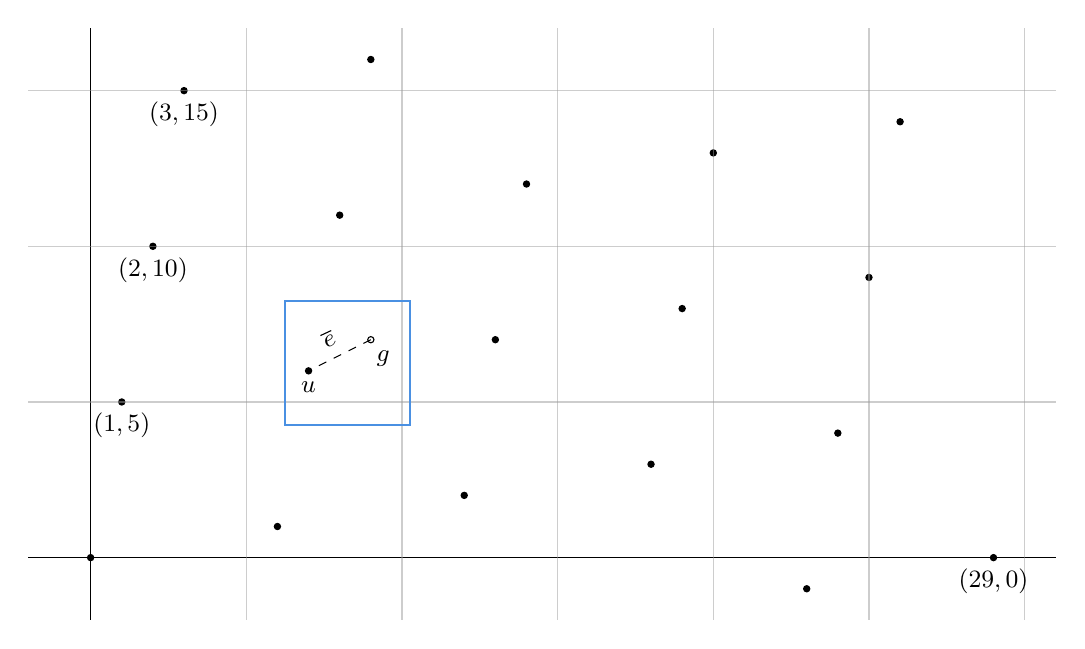
\begin{tikzpicture}[x=0.75pt,y=0.75pt,yscale=-0.75,xscale=0.75]

\draw    (40,0) -- (40,380) ;
\draw    (0,340) -- (660,340) ;

\draw  [fill={rgb, 255:red, 0; green, 0; blue, 0 }  ,fill opacity=1 ] (98,40) .. controls (98,38.9) and (98.9,38) .. (100,38) .. controls (101.1,38) and (102,38.9) .. (102,40) .. controls (102,41.1) and (101.1,42) .. (100,42) .. controls (98.9,42) and (98,41.1) .. (98,40) -- cycle ;
\draw  [fill={rgb, 255:red, 0; green, 0; blue, 0 }  ,fill opacity=1 ] (38,340) .. controls (38,338.9) and (38.9,338) .. (40,338) .. controls (41.1,338) and (42,338.9) .. (42,340) .. controls (42,341.1) and (41.1,342) .. (40,342) .. controls (38.9,342) and (38,341.1) .. (38,340) -- cycle ;
\draw  [fill={rgb, 255:red, 0; green, 0; blue, 0 }  ,fill opacity=1 ] (58,240) .. controls (58,238.9) and (58.9,238) .. (60,238) .. controls (61.1,238) and (62,238.9) .. (62,240) .. controls (62,241.1) and (61.1,242) .. (60,242) .. controls (58.9,242) and (58,241.1) .. (58,240) -- cycle ;
\draw  [fill={rgb, 255:red, 0; green, 0; blue, 0 }  ,fill opacity=1 ] (78,140) .. controls (78,138.9) and (78.9,138) .. (80,138) .. controls (81.1,138) and (82,138.9) .. (82,140) .. controls (82,141.1) and (81.1,142) .. (80,142) .. controls (78.9,142) and (78,141.1) .. (78,140) -- cycle ;
\draw  [fill={rgb, 255:red, 0; green, 0; blue, 0 }  ,fill opacity=1 ] (178,220) .. controls (178,218.9) and (178.9,218) .. (180,218) .. controls (181.1,218) and (182,218.9) .. (182,220) .. controls (182,221.1) and (181.1,222) .. (180,222) .. controls (178.9,222) and (178,221.1) .. (178,220) -- cycle ;
\draw  [fill={rgb, 255:red, 0; green, 0; blue, 0 }  ,fill opacity=1 ] (438,80) .. controls (438,78.9) and (438.9,78) .. (440,78) .. controls (441.1,78) and (442,78.9) .. (442,80) .. controls (442,81.1) and (441.1,82) .. (440,82) .. controls (438.9,82) and (438,81.1) .. (438,80) -- cycle ;
\draw  [fill={rgb, 255:red, 0; green, 0; blue, 0 }  ,fill opacity=1 ] (278,300) .. controls (278,298.9) and (278.9,298) .. (280,298) .. controls (281.1,298) and (282,298.9) .. (282,300) .. controls (282,301.1) and (281.1,302) .. (280,302) .. controls (278.9,302) and (278,301.1) .. (278,300) -- cycle ;
\draw  [fill={rgb, 255:red, 0; green, 0; blue, 0 }  ,fill opacity=1 ] (218,20) .. controls (218,18.9) and (218.9,18) .. (220,18) .. controls (221.1,18) and (222,18.9) .. (222,20) .. controls (222,21.1) and (221.1,22) .. (220,22) .. controls (218.9,22) and (218,21.1) .. (218,20) -- cycle ;
\draw  [fill={rgb, 255:red, 0; green, 0; blue, 0 }  ,fill opacity=1 ] (558,60) .. controls (558,58.9) and (558.9,58) .. (560,58) .. controls (561.1,58) and (562,58.9) .. (562,60) .. controls (562,61.1) and (561.1,62) .. (560,62) .. controls (558.9,62) and (558,61.1) .. (558,60) -- cycle ;
\draw  [fill={rgb, 255:red, 0; green, 0; blue, 0 }  ,fill opacity=1 ] (198,120) .. controls (198,118.9) and (198.9,118) .. (200,118) .. controls (201.1,118) and (202,118.9) .. (202,120) .. controls (202,121.1) and (201.1,122) .. (200,122) .. controls (198.9,122) and (198,121.1) .. (198,120) -- cycle ;
\draw  [fill={rgb, 255:red, 0; green, 0; blue, 0 }  ,fill opacity=1 ] (318,100) .. controls (318,98.9) and (318.9,98) .. (320,98) .. controls (321.1,98) and (322,98.9) .. (322,100) .. controls (322,101.1) and (321.1,102) .. (320,102) .. controls (318.9,102) and (318,101.1) .. (318,100) -- cycle ;
\draw  [fill={rgb, 255:red, 0; green, 0; blue, 0 }  ,fill opacity=1 ] (498,360) .. controls (498,358.9) and (498.9,358) .. (500,358) .. controls (501.1,358) and (502,358.9) .. (502,360) .. controls (502,361.1) and (501.1,362) .. (500,362) .. controls (498.9,362) and (498,361.1) .. (498,360) -- cycle ;
\draw  [fill={rgb, 255:red, 0; green, 0; blue, 0 }  ,fill opacity=1 ] (158,320) .. controls (158,318.9) and (158.9,318) .. (160,318) .. controls (161.1,318) and (162,318.9) .. (162,320) .. controls (162,321.1) and (161.1,322) .. (160,322) .. controls (158.9,322) and (158,321.1) .. (158,320) -- cycle ;
\draw  [fill={rgb, 255:red, 0; green, 0; blue, 0 }  ,fill opacity=1 ] (518,260) .. controls (518,258.9) and (518.9,258) .. (520,258) .. controls (521.1,258) and (522,258.9) .. (522,260) .. controls (522,261.1) and (521.1,262) .. (520,262) .. controls (518.9,262) and (518,261.1) .. (518,260) -- cycle ;
\draw  [fill={rgb, 255:red, 0; green, 0; blue, 0 }  ,fill opacity=1 ] (618,340) .. controls (618,338.9) and (618.9,338) .. (620,338) .. controls (621.1,338) and (622,338.9) .. (622,340) .. controls (622,341.1) and (621.1,342) .. (620,342) .. controls (618.9,342) and (618,341.1) .. (618,340) -- cycle ;
\draw  [fill={rgb, 255:red, 255; green, 255; blue, 255 }  ,fill opacity=1 ] (218,200) .. controls (218,198.9) and (218.9,198) .. (220,198) .. controls (221.1,198) and (222,198.9) .. (222,200) .. controls (222,201.1) and (221.1,202) .. (220,202) .. controls (218.9,202) and (218,201.1) .. (218,200) -- cycle ;
\draw  [fill={rgb, 255:red, 0; green, 0; blue, 0 }  ,fill opacity=1 ] (398,280) .. controls (398,278.9) and (398.9,278) .. (400,278) .. controls (401.1,278) and (402,278.9) .. (402,280) .. controls (402,281.1) and (401.1,282) .. (400,282) .. controls (398.9,282) and (398,281.1) .. (398,280) -- cycle ;
\draw  [fill={rgb, 255:red, 0; green, 0; blue, 0 }  ,fill opacity=1 ] (298,200) .. controls (298,198.9) and (298.9,198) .. (300,198) .. controls (301.1,198) and (302,198.9) .. (302,200) .. controls (302,201.1) and (301.1,202) .. (300,202) .. controls (298.9,202) and (298,201.1) .. (298,200) -- cycle ;
\draw  [fill={rgb, 255:red, 0; green, 0; blue, 0 }  ,fill opacity=1 ] (418,180) .. controls (418,178.9) and (418.9,178) .. (420,178) .. controls (421.1,178) and (422,178.9) .. (422,180) .. controls (422,181.1) and (421.1,182) .. (420,182) .. controls (418.9,182) and (418,181.1) .. (418,180) -- cycle ;
\draw  [fill={rgb, 255:red, 0; green, 0; blue, 0 }  ,fill opacity=1 ] (538,160) .. controls (538,158.9) and (538.9,158) .. (540,158) .. controls (541.1,158) and (542,158.9) .. (542,160) .. controls (542,161.1) and (541.1,162) .. (540,162) .. controls (538.9,162) and (538,161.1) .. (538,160) -- cycle ;


\draw [color={rgb, 255:red, 155; green, 155; blue, 155 }  ,draw opacity=0.5 ][line width=0.5] (140,0) -- (140,380) ;
\draw [color={rgb, 255:red, 155; green, 155; blue, 155 }  ,draw opacity=0.5 ][line width=0.5]   (240,0) -- (240,380) ;
\draw [color={rgb, 255:red, 155; green, 155; blue, 155 }  ,draw opacity=0.5 ][line width=0.5]   (340,0) -- (340,380) ;
\draw [color={rgb, 255:red, 155; green, 155; blue, 155 }  ,draw opacity=0.5 ][line width=0.5]   (440,0) -- (440,380) ;
\draw [color={rgb, 255:red, 155; green, 155; blue, 155 }  ,draw opacity=0.5 ][line width=0.5]   (540,0) -- (540,380) ;
\draw [color={rgb, 255:red, 155; green, 155; blue, 155 }  ,draw opacity=0.5 ][line width=0.5]   (640,0) -- (640,380) ;

\draw [color={rgb, 255:red, 155; green, 155; blue, 155 }  ,draw opacity=0.5 ][line width=0.5]   (0,240) -- (660,240) ;
\draw [color={rgb, 255:red, 155; green, 155; blue, 155 }  ,draw opacity=0.5 ][line width=0.5]   (0,140) -- (660,140) ;
\draw [color={rgb, 255:red, 155; green, 155; blue, 155 }  ,draw opacity=0.5 ][line width=0.5]   (0,40) -- (660,40) ;

\draw  [dash pattern={on 3pt off 3pt}]  (220,200) -- (180,220) ;
\draw  [color={rgb, 255:red, 74; green, 144; blue, 226 }  ,draw opacity=1][line width=0.8]  (165,175) -- (245,175) -- (245,255) -- (165,255) -- cycle ;


\draw (100,45.4) node [anchor=north] [inner sep=0.75pt]  [font=\small]  {$( 3,15)$};
\draw (80,145.4) node [anchor=north] [inner sep=0.75pt]  [font=\small]  {$( 2,10)$};
\draw (60,245.4) node [anchor=north] [inner sep=0.75pt]  [font=\small]  {$( 1,5)$};
\draw (620,345.4) node [anchor=north] [inner sep=0.75pt]  [font=\small]  {$( 29,0)$};
\draw (180,225.4) node [anchor=north] [inner sep=0.75pt]  [font=\small]  {${\boldsymbol u}$};
\draw (222,205.4) node [anchor=north west][inner sep=0.75pt]  [font=\small]  {${\boldsymbol g}$};
\draw (184.94,195.57) node [anchor=north west][inner sep=0.75pt]  [font=\small,rotate=-335]  {$\overline{e}$};


\end{tikzpicture}
	\caption{与攻击LCG相关的二维网格。这里的网格是由向量$(1,5)^\mathrm{T}$和$(0,29)^\mathrm{T}$生成的。攻击者持有向量$\boldsymbol{g}=(9,7)^\mathrm{T}$,并希望找到最接近的网格向量$\boldsymbol{u}$。在这本图中确实只有一个``接近" $\boldsymbol{g}$ 的网格向量。}
	\label{fig:3-9}
\end{figure}

现在,攻击者有一个向量 $\boldsymbol{g}\in\mathbb{Z}^2$,并且知道它的目标向量 $\boldsymbol{u}\in\mathcal{L}_a$ 接近 $\boldsymbol{g}$。如果它能在 $\mathcal{L}_a$ 中找到与 $\boldsymbol{g}$ 最接近的向量,那么这个向量很有可能就是所需的向量 $\boldsymbol{u}$。下面的定理将表明,对于大多数的 $a\in\mathcal{S}_q$ 来说,情况就是如此。
\end{snote}

\begin{lemma}\label{lemma:3-7}
对于 $\mathcal{S}_q$ 上至少 $(1-16/c^2)\cdot q$ 个 $a$,网格 $\mathcal{L}_a\subseteq\mathbb{Z}^2$ 有如下性质:对于每个 $\boldsymbol{g}\in\mathbb{Z}^2$,最多只存在一个向量 $\boldsymbol{u}\in\mathcal{L}_a$ 满足 $\lVert\boldsymbol{g}-\boldsymbol{u}\rVert_\infty < \sqrt{q}/c$。
\end{lemma}

在引理 \ref{lemma:3-7} 中取 $c=32$(则 $w=\sqrt{q}/30$),那么对于 $98\%$ 的 $a\in\mathcal{S}_q$ 来说,$\mathcal{L}_a$ 上离 $\boldsymbol{g}$ 最近的向量恰好就是所需的向量 $\boldsymbol{u}$。在证明该引理之前,我们首先完成对攻击的描述。

剩下的工作就是有效地找到 $\mathcal{L}_a$ 上离 $\boldsymbol{g}$ 最近的向量。这个问题是一个更一般的问题的特例,它叫做\textbf{最近向量问题(closest vector problem)}:给定一个网格 $\mathcal{L}$ 和一个向量 $\boldsymbol{g}$,找到 $\mathcal{L}$ 上离 $\boldsymbol{g}$ 最近的向量。有了这个算法,攻击者就可以根据生成器的两个输出 $r_i$ 和$r_{i+1}$ 恢复 LCG 的内部状态 $s_i$,并预测剩余的序列。这种攻击对 $98\%$ 的 $a\in\mathcal{S}_q$ 都有效。

完整起见,我们注意到,在剩下的 $2\%$ 中,一些 $a\in\mathcal{S}_q$ 所发起的攻击会失败,比如 $a=1$ 和 $a=2$。对于这些 $a$,在 $\mathcal{L}_a$ 上可能会有多个接近给定的 $\boldsymbol{g}$ 的网格向量。我们把设计一个对于 $\mathcal{S}_q$ 上那些不适用于引理 \ref{lemma:3-7} 的 $a$ 有效的攻击作为一个有趣的练习。最后,我们证明引理 \ref{lemma:3-7},以此来结束本小节。

\begin{proof}[引理 \ref{lemma:3-7} 的证明]
令 $\boldsymbol{g}\in\mathbb{Z}^2$,假设 $\mathcal{L}_a$ 中存在两个接近 $\boldsymbol{g}$ 的向量 $\boldsymbol{u}_0$ 和 $\boldsymbol{u}_1$,即 $\lVert\boldsymbol{u}_i-\boldsymbol{g}\rVert_\infty<\sqrt{q}/c$ 对于 $i=0,1$ 都成立。那么 $\boldsymbol{u}_0$ 和 $\boldsymbol{u}_1$ 一定是相互接近的。事实上,根据三角不等式,我们有:
\[
\lVert\boldsymbol{u}_0-\boldsymbol{u}_1\rVert_\infty
\leq
\lVert\boldsymbol{u}_0-\boldsymbol{g}\rVert_\infty
+\lVert\boldsymbol{g}-\boldsymbol{u}_1\rVert_\infty
\leq
2\sqrt{q}/c
\]
由于任何网格在加法下都是封闭的,我们可以看出 $\boldsymbol{u}:=\boldsymbol{u}_0-\boldsymbol{u}_1$ 也是网格 $\mathcal{L}_a$ 中的一个向量,并且我们可以得出结论:$\mathcal{L}_a$ 中一定包含一个``短的"向量,即一个范数最大为 $B:= 2\sqrt{q}/c$ 的非零向量。因此,我们对使得 $\mathcal{L}_a$ 包含这样一个短向量的``坏的" $a$ 的数量进行约束。

我们首先考虑 $q$ 是素数的情况。我们声称,每个短向量最多只会被包含在一个网格 $\mathcal{L}_a$ 中,因此坏的 $a$ 的数量不会超过短向量的数量。假设 $\boldsymbol{t}=(s,y)^\mathrm{T}\in\mathbb{Z}^2$ 是某个非零向量,满足 $\lVert\boldsymbol{t}\rVert_\infty\leq B$。假设对于某个 $a\in\mathcal{S}_q$,我们有 $\boldsymbol{t}\in\mathcal{L}_a$,则必然存在整数 $s_a$ 和 $x_a$ 使得 $s_a\cdot(1,a)^\mathrm{T}+x_a\cdot(0,q)^\mathrm{T}=\boldsymbol{t}=(s,y)^\mathrm{T}$ 成立。由此我们可得 $s=s_a$ 和 $y=as\bmod q$。此外,我们还有 $s\neq0$,因为如果不是这样,我们就有 $\boldsymbol{t}=\boldsymbol{0}$。但是由于 $y=as\bmod q$,且 $s\neq0$,$a$ 的值是唯一确定的,即 $a=ys^{-1}\bmod q$。因此,当 $q$ 是素数时,每个非零的短向量 $\boldsymbol{t}$ 最多都只包含在一个 $a\in\mathcal{S}_q$ 的网格中。进而可知,坏的 $a$ 的数量不会超过短向量的数量,即 $(2B)^2=16q/c^2$。

当 $q$ 不是素数时,对坏的 $a$ 的数量的约束同样成立。为了说明原因,考虑一个特定的非零 $s\in\mathcal{S}_q$,并令 $d=\gcd(s, q)$。如上所述,只有当存在一个 $a\in\mathcal{S}_q$ 满足 $as\equiv y\,(\bmod\,q)$ 时,向量 $\boldsymbol{t}=(s,y)^\mathrm{T}$ 才会被包含在某个网格 $\mathcal{L}_a$ 中。这意味着 $y$ 必须是 $d$ 的整数倍,所以我们只需要考虑 $y$ 的 $2B/d$ 个可能取值。对于每个这样的 $y$,向量 $\boldsymbol{t}=(s,y)^\mathrm{T}$ 最多都只会被包含在 $d$ 个网格中。由于 $s$ 有 $2B$ 种可能取值,这就表明坏的 $a$ 的数量以 $d\cdot 2B/d \cdot 2B=(2B)^2$ 为上界,这与 $q$ 是素数的情况相同。

总之,$\mathcal{S}_q$ 中最多有 $16q/c^2$ 个坏的 $a$。因此,对于 $\mathcal{S}_q$ 中的 $(1-16/c^2)\cdot q$ 个 $a$ 的取值,网格 $\mathcal{L}_a$ 中都不包含非零短向量,故而该引理得证。
\end{proof}

\subsection{子集和生成器}

接下来,我们介绍如何基于简单的线性运算构建一个伪随机生成器。假设经典\emph{子集和问题(subset sum problem)}的某个随机化版本是困难的,则这个生成器就是安全的。

\begin{snote}[模子集问题。]
令 $q$ 是一个正整数,令 $\mathcal{S}_q:=\{0,\dots,q-1\}$。在 $\mathcal{S}_q$ 中选择 $n$ 个整数 $\boldsymbol{a}:=(a_0,\dots,a_{n-1})$,并定义子集和函数 $f_{\boldsymbol{a}}:\{0,1\}^n\to\mathcal{S}_q$ 如下:
\[
f_{\boldsymbol{a}}(\boldsymbol{s})
:=\sum_{i: s_i=1}a_i\bmod q
\]
例如,$f_{\boldsymbol{a}}(101101)=a_0+a_1+a_2+a_4\bmod q$。现在,对于一个目标整数 $t\in\mathcal{S}_q$,模子集问题的定义如下:
\begin{quote}
给定 $(q,\boldsymbol{a},t)$ 作为输入,如果存在一个向量 $\boldsymbol{s}\in\{0,1\}^n$ 满足 $f_{\boldsymbol{a}}(\boldsymbol{s})=t$,就将其输出。
\end{quote}
换句话说,该问题是,如果函数 $f_{\boldsymbol{a}}(\cdot)$ 存在反函数,就通过寻找 $t$ 的原像的方式来求得该反函数。模子集问题目前被认为是 $\mathcal{NP}$ 困难的。
\end{snote}

\begin{snote}[子集和与PRG。]
子集问题能够自然地导出下面的 PRG:在设置阶段,选择一个固定整数 $q$,并从 $\mathcal{S}_q$ 中随机选择 $n$ 个整数 $\vec{a}:=(a_0,\dots,a_{n-1})$。PRG $G_{q,\vec{a}}$ 将一个种子 $\boldsymbol{s}\in\{0,1\}^n$ 作为输入,并输出一个 $\mathcal{S}_q$ 上的伪随机值。其定义为:
\[
G_{q,\vec{a}}(\boldsymbol{s})
:=\sum_{i=1}^na_i\cdot s_i\bmod q
\]
该 PRG 将一个 $n$ 比特的种子拉伸为一个 $\log_2q$ 比特的输出。选择 $n$ 和 $q$ 使得 $2n=\log_2q$,我们就可以得到一个 PRG,其输出长度是输入长度的两倍。我们可以将其插入 Blum-Micali 构造中以进一步拉长输出。

虽然这个 PRG 比 \ref{sec:3-6} 节中介绍的 ChaCha20 等自定义构造要慢得多,但每一位输出所对应的工作都只是 $\mathcal{S}_q$ 上的一个模加法,这可能适合一些对时间不敏感的应用。

Impagliazzo 和 Naor 表明,攻击基于 $G_{q,\vec{a}}$ 的 PRG 的难度与解决模子集和问题的某个随机化变体一致 \cite{impagliazzo1996efficient}。尽管已经有很多工作试图解决模子集问题,但对于较大的 $n$,比如 $n>1000$,当 $2n=\log_2q$ 时,该问题似乎仍然是很难的,这就意味着 $G_{q,\vec{a}}$ 作为一个 PRG 仍然是安全的。
\end{snote}

\begin{snote}[变体。]
Fischer 和 Stern 提出了下面这种子集和生成器的变体 \cite{fischer1996efficient}:
\[
G_{q,A}(\boldsymbol{s})
:=A\cdot\boldsymbol{s}\bmod q
\]
其中,$q$ 是一个小素数,$A$ 是一个 $\mathcal{S}_q^{n\times m}$ 上的随机矩阵,$n<m$,并且种子 $\boldsymbol{s}$ 均匀分布在 $\{0,1\}^m$ 上。该生成器将 $m$ 比特的种子映射为 $n\log_2q$ 比特的输出。我们将在第\ref{chap:16}章进一步讨论这个生成器。
\end{snote}
\section{案例研究:对DVD加密系统的密码学分析}\label{sec:3-8}

内容加扰系统 (Content Scrambling System, CSS) 是一个用于保护 DVD 光盘上的电影的系统。它使用一种称为 CSS 的流密码来加密电影内容。CSS 设计于 20 世纪 80 年代,当时,可出口的加密算法被限制在 $40$ 比特密钥以内。因此,CSS 使用 $40$ 比特的密钥对电影进行加密。虽然我们现在已经知道,使用 $40$ 比特密钥的密码是非常不安全的,但我们将表明,CSS 流密码格外弱,以至于我们可以找到比穷举所有 $2^{40}$ 个密钥耗时更短的破解方法。它为密码分析提供了一个有趣的机会。

\begin{snote}[线性反馈移位寄存器(Linear feedback shift register, LFSR)。]
CSS 流密码由两个 LFSR 构建。一个 $n$ 比特 LFSR 由一组整数 $V:=\{v_1,\dots,v_d\}$ 定义,其中每个 $v_i$ 都在 $\{0,\dots,n-1\}$ 区间内。$V$ 中的元素被称为\textbf{抽头位置 (tap position)}。一个 LFSR 能够提供一个 PRG(见图 \ref{fig:3-10}),如下所述:

\vspace*{10pt}

\hspace*{5pt} 输入:$s=(b_{n-1},\dots,n_0)\in\{0,1\}^n$,其中$s\neq 0^n$\\
\hspace*{26pt} 输出:$y\in\{0,1\}^\ell$,其中$\ell>n$

\vspace*{5pt}

\hspace*{5pt} 对于 $i\leftarrow1\dots\ell$:\\
\hspace*{26pt} \quad\quad\quad 输出 $b_0$
\hspace*{86.5pt} // \emph{输出一比特}\\
\hspace*{26pt} \quad\quad\quad $b\leftarrow b_{v_1}\oplus\cdots\oplus b_{v_d}$
\hspace*{34.5pt} // \emph{计算反馈比特}\\
\hspace*{26pt} \quad\quad\quad $s\leftarrow(b,\,b_{n-1},\,\dots,\,b_1)$
\hspace*{22.5pt} // \emph{将寄存器中的比特右移}

\vspace*{10pt}

\noindent
LFSR 每个时钟周期输出一个比特。请注意,如果一个 LFSR 在启动时状态为 $s=0^n$,那么它的输出会退化为全 $0$。由于这个原因,种子中的某一比特必须总是被置为 $1$。

LFSR 可以用很少的晶体管在硬件上实现。因此,由 LFSR 构建的流密码对于低成本的消费电子产品(如 DVD 播放器、手机和蓝牙设备)很有吸引力。
\end{snote}

\begin{figure}
	\centering
	

\tikzset{every picture/.style={line width=0.75pt}} %set default line width to 0.75pt        

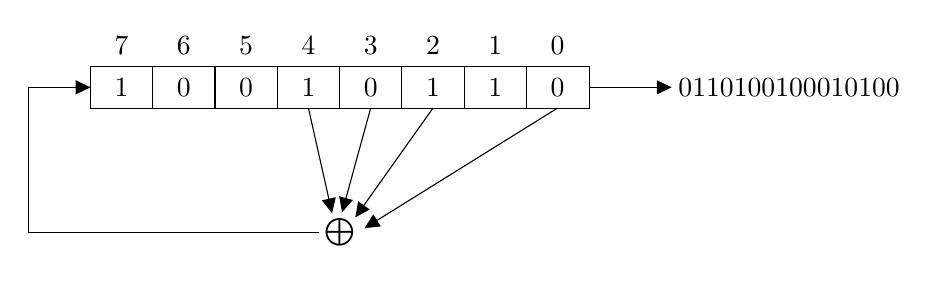
\begin{tikzpicture}[x=0.75pt,y=0.75pt,yscale=-1,xscale=1]
%uncomment if require: \path (0,120); %set diagram left start at 0, and has height of 120

%Shape: Rectangle [id:dp8699898407336639] 
\draw   (60,20) -- (300.4,20) -- (300.4,40) -- (60,40) -- cycle ;
%Straight Lines [id:da6480423944948943] 
\draw    (90,20) -- (90,40) ;
%Straight Lines [id:da1357097181943394] 
\draw    (120,20) -- (120,40) ;
%Straight Lines [id:da6348473634558065] 
\draw    (150,20) -- (150,40) ;
%Straight Lines [id:da9852363854962749] 
\draw    (180,19.97) -- (180,40) ;
%Straight Lines [id:da6251188632523177] 
\draw    (210,20) -- (210,40) ;
%Straight Lines [id:da9628068129583953] 
\draw    (240,20) -- (240,40) ;
%Straight Lines [id:da5093234988477329] 
\draw    (270,20) -- (270,40) ;
%Straight Lines [id:da506886279614565] 
\draw    (165,40) -- (175.74,87.74) ;
\draw [shift={(176.4,90.67)}, rotate = 257.32] [fill={rgb, 255:red, 0; green, 0; blue, 0 }  ][line width=0.08]  [draw opacity=0] (7.14,-3.43) -- (0,0) -- (7.14,3.43) -- cycle    ;
%Straight Lines [id:da08239608836085877] 
\draw    (195,40) -- (181.99,87.38) ;
\draw [shift={(181.2,90.27)}, rotate = 285.35] [fill={rgb, 255:red, 0; green, 0; blue, 0 }  ][line width=0.08]  [draw opacity=0] (7.14,-3.43) -- (0,0) -- (7.14,3.43) -- cycle    ;
%Straight Lines [id:da8508423498295425] 
\draw    (225,40) -- (189.34,90.22) ;
\draw [shift={(187.6,92.67)}, rotate = 305.38] [fill={rgb, 255:red, 0; green, 0; blue, 0 }  ][line width=0.08]  [draw opacity=0] (7.14,-3.43) -- (0,0) -- (7.14,3.43) -- cycle    ;
%Straight Lines [id:da1889764527983564] 
\draw    (285,40) -- (194.55,96.28) ;
\draw [shift={(192,97.87)}, rotate = 328.11] [fill={rgb, 255:red, 0; green, 0; blue, 0 }  ][line width=0.08]  [draw opacity=0] (7.14,-3.43) -- (0,0) -- (7.14,3.43) -- cycle    ;
%Straight Lines [id:da2853178114885824] 
\draw    (170,100) -- (30,100) -- (30,30) -- (57,30) ;
\draw [shift={(60,30)}, rotate = 180] [fill={rgb, 255:red, 0; green, 0; blue, 0 }  ][line width=0.08]  [draw opacity=0] (7.14,-3.43) -- (0,0) -- (7.14,3.43) -- cycle    ;
%Straight Lines [id:da8823488045232695] 
\draw    (300,30) -- (337,30) ;
\draw [shift={(340,30)}, rotate = 180] [fill={rgb, 255:red, 0; green, 0; blue, 0 }  ][line width=0.08]  [draw opacity=0] (7.14,-3.43) -- (0,0) -- (7.14,3.43) -- cycle    ;

% Text Node
\draw (75,30) node    {$1$};
% Text Node
\draw (105,29.97) node    {$0$};
% Text Node
\draw (135,30) node    {$0$};
% Text Node
\draw (165,30) node    {$1$};
% Text Node
\draw (195,30) node    {$0$};
% Text Node
\draw (225,30) node    {$1$};
% Text Node
\draw (255,30) node    {$1$};
% Text Node
\draw (285,30) node    {$0$};
% Text Node
\draw (75,10) node    {$7$};
% Text Node
\draw (105,10) node    {$6$};
% Text Node
\draw (135,10) node    {$5$};
% Text Node
\draw (165,10) node    {$4$};
% Text Node
\draw (195,10) node    {$3$};
% Text Node
\draw (225,10) node    {$2$};
% Text Node
\draw (255,10) node    {$1$};
% Text Node
\draw (285,10) node    {$0$};
% Text Node
\draw (180,100) node  [font=\large]  {$\bigoplus $};
% Text Node
\draw (342,30) node [anchor=west] [inner sep=0.75pt]    {$0110100100010100\dotsc $};


\end{tikzpicture}
	\caption{$8$比特的线性反馈移位寄存器$\{4,3,2,0\}$}
	\label{fig:3-10}
\end{figure}

\begin{snote}[来自 LSFR 的流密码。]
一个单一的 LFSR 作为 PRG 是完全不安全的,因为给定其输出的 $n$ 个连续比特,很容易就能计算出所有的后续比特。然而,使用一个非线性组件把几个 LFSR 组合起来,我们就有可能得到在某种程度上(弱)安全的 PRG。一种属于 eStream 组合的流密码 Trivium 就是这样构建出来的。

从 LFSR 构建流密码的一种方法是并行地运行几个 LFSR,并使用非线性操作组合它们的输出。接下来描述的 CSS 流密码使用整数域上的加法将两个 LFSR 组合起来。而被用于加密 GSM 手机流量的 A5/1 流密码组合了三个 LFSR 的输出。蓝牙 E0 流密码使用一个 $2$ 比特的有限状态机将四个 LFSR 组合起来。所有这些算法都已经被证明是不安全的,并且不应该再被使用。这是因为对于这些密码,恢复明文所需的时间远远少于对密钥空间进行穷举搜索的耗时。

另一种方法是只运行一个 LFSR,并对其内部状态进行非线性操作来产生输出。用于加密 3GPP 手机流量的 \texttt{snow} 3G 密码就是这样操作的。
\end{snote}

\begin{snote}[CSS 流密码。]
CSS 流密码是由图 \ref{fig:3-11} 所示的 PRG 构建的。该 PRG 的工作原理如下:

\vspace*{10pt}

\hspace*{5pt} 输入:种子 $s\in\{0,1\}^{40}$\\
\hspace*{26pt} 输出:$\ell$ 个比特

\vspace{5pt}

\hspace*{5pt} 令 $s=s_1\,\Vert\,s_2$,其中 $s_1\in\{0,1\}^{16}$,$s_2\in\{0,1\}^{24}$\\
\hspace*{26pt} 将 $1\,\Vert\,s_1$ 加载到一个 $17$ 比特的 LFSR 中\\
\hspace*{26pt} 将 $1\,\Vert\,s_2$ 加载到一个 $25$ 比特的 LFSR 中\\
\hspace*{26pt} 令 $c\leftarrow 0$ \quad\quad // \emph{进位}\\
\hspace*{26pt} 对于 $i=1,\dots,\ell$:\\
\hspace*{50pt} 将两个 LFSR 运行 $8$ 个周期,得到 $x_i,y_i\in\{0,1\}^8$\\
\hspace*{50pt} 将 $x_i$ 和 $y_i$ 视作 $\{0,\dots,255\}$ 中的两个整数\\
\hspace*{50pt} 输出 $z_i:=x_i+y_i+c\bmod 256$\\
\hspace*{50pt} 如果 $x_i+y_i>255$,则令 $c\leftarrow1$,否则令 $c\leftarrow0$ \quad\quad // \emph{进位}

\vspace*{10pt}

该 PRG 每次迭代输出一个字节。在 $s_1$ 和 $s_2$ 中预留的 $1$ 确保 LFSR 不会被初始化为全 $0$ 状态。两个 LFSR 的抽头是固定的。$17$ 比特的 LFSR 使用的是抽头 $\{14,0\}$,25比特的 LFSR 使用抽头 $\{12,4,3,0\}$。

我们展示的 CSS PRG 是 CSS 的一个小变体,它描述起来比较容易,但和真正的 CSS 具有同等的安全性。在真正的 CSS 中,对于 $17$ 比特的 LFSR,我们不是在初始种子中预置 $1$,而是在第 $9$ 比特的位置插入 $1$;而对于 $25$ 比特的 LFSR,是在第 $22$ 比特处插入 $1$。此外,真正的 CSS 会丢弃 $17$ 比特 LFSR 输出的第一个字节和 $25$ 比特 LFSR 输出的前两个字节。这两个问题都不会影响到接下来的分析。
\end{snote}

\begin{figure}
	\centering
	\tikzset{every picture/.style={line width=0.75pt}}      

\begin{tikzpicture}[x=0.75pt,y=0.75pt,yscale=-0.9,xscale=0.9]

\draw   (60,20) -- (300,20) -- (300,40) -- (60,40) -- cycle ;
\draw   (0,100) -- (300,100) -- (300,120) -- (0,120) -- cycle ;

\draw  [fill={rgb, 255:red, 255; green, 255; blue, 255 }  ,fill opacity=1 ][general shadow={fill={rgb, 255:red, 0; green, 0; blue, 0 }  ,shadow xshift=2pt,shadow yshift=-2pt, opacity=1 }] (280,60) -- (480,60) -- (480,80) -- (280,80) -- cycle ;

\draw  [->]  (300,30) -- (380,30) -- (380,59) ;
\draw  [->]  (300,110) -- (380,110) -- (380,83) ;
\draw  [->]  (480,70) -- (550,70) ;

\draw (180.2,30) node   [align=left][font=\small] {$17$-bit LFSR};
\draw (150,110) node   [align=left][font=\small] {$25$-bit LFSR};
\draw (380,70) node  [font=\small]  {$x+y+c\bmod 256$};
\draw (340,113) node [anchor=north] [inner sep=0.75pt][align=left][font=\footnotesize] {$8$ bits};
\draw (340,27) node [anchor=south] [inner sep=0.75pt][align=left][font=\footnotesize] {$8$ bits};
\draw (382,45) node [anchor=west] [inner sep=0.75pt][font=\footnotesize]    {$x$};
\draw (382,95) node [anchor=west] [inner sep=0.75pt][font=\footnotesize]    {$y$};
\draw (515.17,73.4) node [anchor=north] [inner sep=0.75pt][font=\footnotesize]    {$8$};

\end{tikzpicture}
	\caption{CSS流密码}
	\label{fig:3-11}
\end{figure}

\begin{snote}[CSS的不安全性。]
给定 PRG 的输出,通过对种子空间进行穷举搜索,我们显然可以在 $2^{40}$ 次计算内恢复秘密的种子。我们下面展示一种更快的攻击方法,它只需要进行 $2^{16}$ 次猜测。假设我们得到了 PRG 输出的前 $100$ 字节 $\bar{z}:=(z_1,z_2,\dots)$。该攻击基于以下观察:
\begin{quote}
令 $(x_1,x_2,x_3)$ 和 $(y_1,y_2,y_3)$ 分别为 $17$ 比特和 $25$ 比特 LFSR 输出的前 $3$ 字节。则有:
\[
(2^{16}x_3+2^8x_2+x_1)+(2^{16}y_3+2^8y_2+y_1)
\equiv(2^{16}z_3+2^8z_2+z_1)\;\;(\bmod\;2^{24})
\]
因此,一旦已知 $(z_1,z_2,z_3)$ 和 $(x_1,x_2,x_3)$,我们就很容易算出 $(y_1,y_2,y_3)$,进而很容易得到 $25$ 比特 LFSR 的初始状态 $s_2$。
\end{quote}
有了这个观察,攻击者就可以尝试 $s_1$ 的所有 $16$ 比特可能值,以此恢复种子 $s$。对于每个 $s_1$ 的猜测,攻击者计算出 $17$ 比特 LFSR 对应的输出 $(x_1,x_2,x_3)$。利用上面的观察,它就能够获得一个 $25$ 比特 LFSR 的候选种子 $s_2$。然后,为了确认 $\hat{s}:=s_1\Vert s_2$ 是否是正确的秘密种子,它使用种子 $\hat{s}$ 运行 PRG 的 $100$ 次迭代,并将输出的结果与给定的序列 $\bar{z}$ 进行比较。如果序列不匹配,就换一个 $s_1$ 重新进行计算。一旦攻击者找到了正确的 $s_1$,生成的序列就会与给定的 $\bar{z}$ 一致,在这种情况下,攻击者就得到了正确的秘密种子 $\hat{s}:=s_1\,\Vert\,s_2$。

我们上面的分析表明,对 $s_1$ 进行预计大概 $2^{15}$ 次猜测后,我们就可以恢复整个种子 $s$。这比单纯地进行 $2^{40}$ 次穷举搜索攻击要快得多。
\end{snote}
\section{案例研究:对RC4流密码的密码学分析}

RC4流密码由Ron Rivest在1987年设计,历史上曾用于保护网络流量(在SSL/TLS协议中)和无线流量(在802.11b WEP协议中)的安全。它被设计为可在内存很小的$8$位处理器上运行。虽然RC4仍在使用,但它已被证明容易遭受一些显著的攻击,因而不应该被应用在新的项目中。我们对RC4的讨论可以作为流密码分析的一个优雅的例子。

RC4密码的核心是一个PRG,称为RC4 PRG。PRG维护一个内部状态,包含一个$256$字节的数组$S$和两个额外的字节$i,j$,作为指入$S$的两个指针。数组$S$包含$\{0,\dots,255\}$中的所有的数字,且每个数字正好出现一次。图 \ref{fig:3-12} 给出了一个 RC4 状态的例子。

\begin{figure}
  \centering
  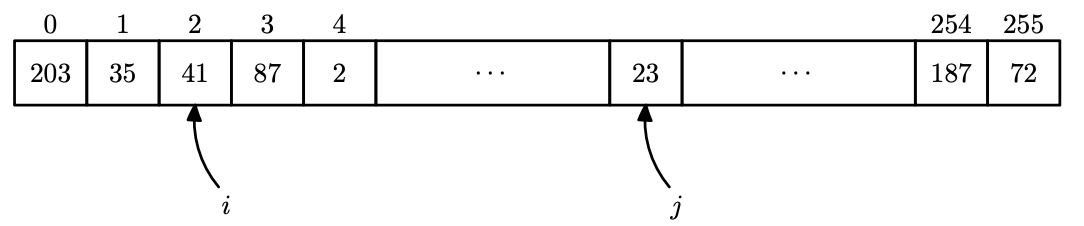
\includegraphics[width=0.75\linewidth]{figures/chapter3/fig12.png}
  \caption{RC4内部状态的一个例子}
  \label{fig:3-12}
\end{figure}

RC4流密码的密钥 $s$ 也是 PRG 的种子,用于将数组 $S$ 初始化为数字 $0 \dots 255$ 一个伪随机置换排列。初始化是使用下面的\textbf{设置算法(setup algorithm)}进行的:

\vspace*{5pt}

\hspace*{5pt} 输入:字节序列$s$

\vspace{3pt}

\hspace*{5pt} 对于 $i=1,\dots,255$:\\
\hspace*{50pt} 令 $S[i]\leftarrow i$ \\
\hspace*{26pt} 令 $j\leftarrow0$\\
\hspace*{26pt} 对于 $i=1,\dots,255$:\\
\hspace*{50pt} 令 $k\leftarrow s[i\;\mathrm{mod}\;|s|]$ \quad\quad // \emph{从种子中提取一个字节}\\
\hspace*{50pt} 令 $j\leftarrow(j+S[i]+k)\;\mathrm{mod}\;256$\\
\hspace*{50pt} $\mathrm{swap}(S[i],S[j])$

\vspace*{5pt}

在循环过程中,索引 $i$ 在数组中线性增长,而索引 $j$ 则跳来跳去。在每次迭代中,指针 $i$ 所指向的内容都会与 $j$ 所指向的内容互换。

一旦数组 $S$ 被初始化,PRG 就可以使用下面的\textbf{流生成器(stream generator)}一次生成一个字节的伪随机输出:

\vspace*{5pt}

\hspace*{5pt} 令 $i\leftarrow0$,$j\leftarrow0$\\
\hspace*{26pt} 重复:\\
\hspace*{50pt} 令 $i\leftarrow(i+1) \;\mathrm{mod}\;256$\\
\hspace*{50pt} 令 $j\leftarrow(j+S[i])\;\mathrm{mod}\;256$\\
\hspace*{50pt} $\mathrm{swap}(S[i],S[j])$ \\
\hspace*{50pt} 输出 $S\big[\,(S[i]+S[j])\;\mathrm{mod}\;256\,\big]$ \\
\hspace*{26pt} 直到永远

\vspace*{5pt}

该程序的运行时间视需要而定。同样地,索引 $i$ 在数组中线性增长,而索引 $j$ 则跳来跳去。交换 $S[i]$ 和 $S[j]$ 会不断地打乱数组 $S$。

\begin{snote}[RC4的加密速度。]
RC4 很适合用软件实现。其他流密码,如 Grain 和 Trivium,是为硬件设计的,在软件实现下的性能表现很差。表 \ref{tab:3-1} 提供了 RC4 和其他一些软件实现的流密码的运行时间对比。现代处理器运行在 $64$ 比特字长上,使得基于 $8$ 比特设计的 RC4 在这些架构上稍显缓慢。
\end{snote}

\begin{table}
  \centering
  \begin{tabular}{|c|c|}
    \hline
    密码 & 速度\footnotemark[1](MB/s)\\
    \hline
    RC4 & 126\\
    SEAL & 375\\
    Salsa20 & 408\\
    Sosemanuk & 727\\
    \hline
  \end{tabular}
  \caption{软件实现的流密码的速度比较(速度越高越好)。}
\end{table}

\subsection{RC4的安全性}

\footnotetext[1]{性能数字是使用 Crypto++ 5.6.0 benchmark 在 1.83 Ghz Intel Core 2 处理器上运行获得的。}

RC4一度被认为是一个安全的流密码,并被广泛部署在应用程序中。在一些攻击表明它的输出有一定的偏差后,该密码就失宠了。我们下面提出两种攻击,它们都能将 RC4 的输出与随机字符串区分开来。在本小节中,我们用$n$表示数组$S$的大小。对于RC4,我们有$n=256$。

\begin{snote}[初始 RC4 输出中的偏差。]
RC4的设置算法基于给定的随机种子将数组$S$初始化为$0 \dots 255$的一个置换。我们先暂且假设 RC4 的设置算法是完美的,它能从所有可能的 $256!$ 个排列组合中产生一个均匀的置换排列。Mantin和Shamir表明,即使假设初始化是完美的,RC4 的输出也是有偏差的。
\end{snote}

\begin{lemma}[Mantin-Shamir定理]\label{lemma:3-8}
假设数组 $S$ 被设置为 $0\dots n-1$ 的一个随机排列,并且 $i$ 和 $j$ 都被置为 $0$,那么 RC4 输出的第二个字节等于 $0$ 的概率为 $2/n$。
\end{lemma}

\begin{proof}[证明思路]
令$z_2$是 RC4 输出的第二个字节。令 $P$ 是 $S[2]=0$和 $S[1]\neq2$ 成立的事件。关键的观察是,当事件 $P$ 发生时,$z_2=0$ 的概率为 $1$,见图 \ref{fig:3-13}。然而,当 $P$ 没有发生时,$z_2$ 均匀分布在 $0\dots n-1$ 上,因此它等于 $0$ 的概率为 $1/n$。由于 $\Pr[P]$ 约为 $1/n$,我们可以得到以下(近似)结果:
\[
\begin{aligned}
\Pr[z_2=0] & =\Pr[(z_2=0)\;|\;P]\cdot\Pr[P]+\Pr[(z_2=0)\;|\;\neg P]\cdot\Pr[\neg P]\\
& \approx 1\cdot(1/n)+(1/n)\cdot(1-1/n)\approx2/n\qedhere
\end{aligned}
\]
\end{proof}

该引理表明,RC4输出的第二个字节为 $0$ 的概率是它本应有的两倍。这就导出了一个简单的 RC4 PRG 区分器。给定一个序列$x\in\{0,\dots,255\}^\ell$,对于$\ell\geq2$,如果$x$的第二个字节是$0$,区分器输出$0$,否则就输出$1$。根据引理 \ref{lemma:3-8},这个区分器的优势约为 $1/n$,对于 RC4 来说就是 $0.39\%$。

\begin{figure}
  \centering
  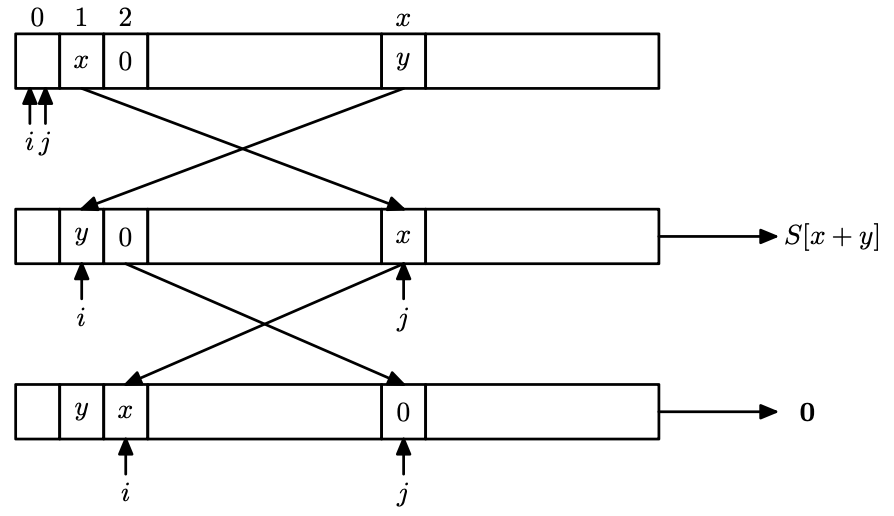
\includegraphics[width=0.55\linewidth]{figures/chapter3/fig13.png}
  \caption{引理 \ref{lemma:3-8} 的证明}
  \label{fig:3-13}
\end{figure}

Mantin-Shamir 区分器表明 RC4 输出的第二字节是有偏差的。AlFardan等人推广了这一结论,他们通过测量许多随机密钥上的偏差,表明输出的前$256$个字节中的每一个都有偏差:每个字节的分布都与均匀性相差甚远。这种偏差不像第二字节那样明显,但它仍是不可忽略不计的,足以用来对密码发动攻击。例如,他们表明,给定用 $2^{30}$ 个随机密钥加密的单一明文的对应密文,我们有可能以接近 $1$ 的概率恢复明文的前 $128$ 字节。这种攻击很容易在网络上进行,因为在网络上,一个秘密的 cookie 通常被嵌入到一个消息的前几个字节中。每次浏览器连接到受害者的网络服务器时,这个 cookie 都会用新的密钥重新加密。攻击者可以使用 Javascript 脚本令用户的浏览器反复重连到目标网站,以向攻击者提供发动攻击和暴露 cookie 所需的 $2^{30}$ 个密文。

作为回应,RSA实验室发布了一项建议,建议放弃RC4流生成器输出的前 $1024$ 字节,而只使用第 $1025$ 字节及以后的字节。这可以防御最初的密钥流偏差区分器,但不能防御我们接下来将要讨论的攻击。

\begin{snote}[RC4流生成器中的偏差。]
假设RC4设置算法已经被修改,从而使得上面介绍的攻击无效。Fluhrer和McGrew给出了一个直接针对流生成器的攻击。他们声称字节对$(0,0)$ 在 RC4 的输出中出现的次数多于它应该在随机序列中出现的次数。这足以将 RC4 的输出与随序列区分开来。

令 $\mathrm{ST}_\mathrm{RC4}$ 为 RC4 所有可能的内部状态的集合。由于数组 $S$ 有 $n$ 个可能的设置,$i$ 和 $j$ 各有 $n$ 个可能的设置,所以 $\mathrm{ST}_\mathrm{RC4}$ 的大小为 $n!\cdot n^2$。由于在 RC4 中$n=256$,$\mathrm{ST}_\mathrm{RC4}$ 的大小是非常巨大的,大约为 $10^{511}$。
\end{snote}

\begin{lemma}[Fluhrer-McGrew定理]
假设RC4使用一个$\mathrm{ST}_\mathrm{RC4}$中的随机状态$T$初始化。令$(z_1,z_2)$是 RC4 在状态 $T$ 下启动时输出的前两个字节。则有:
\[
\begin{aligned}\label{lemma:3-9}
& i\neq n−1 & \Longrightarrow & \quad\Pr[(z_1,z_2)=(0,0)]\geq(1/n^2)\cdot\big(1+(1/n)\big)\\
& i\neq 0,1 & \Longrightarrow & \quad\Pr[(z_1,z_2)=(0,1)]\geq(1/n^2)\cdot\big(1+(1/n)\big)
\end{aligned}
\]
\end{lemma}

我们将一对连续输出 $(z_1,z_2)$ 称为一个\textbf{二重字(digraph)}。在一个真正的随机序列中,所有二重字$(x,y)$出现的概率都应当正好是 $1/n^2$。上面的引理表明,对于RC4,$(0,0)$出现的概率比它应有的值大$1/n^3$。$(0,1)$也是如此。事实上,除了引理 \ref{lemma:3-9} 所述的两个二重字,Fluhrer-McGrew 还确定了其他几个异常的二重字。

该引理导出了一个简单的区分 RC4 的输出和随机序列的区分器 $D$。如果区分器在给定的序列中发现的 $(0,0)$ 的数量大于随机序列中应有的数量,它就输出 $1$,否则就输出 $0$。

\vspace*{5pt}

\hspace*{5pt} 输入:序列$s\in\{0,\dots,n\}^\ell$\\
\hspace*{26pt} 输出:$0$ 或 $1$

\vspace{3pt}

\hspace*{5pt} 令 $q$ 为 $x$ 中出现二重字 $(0,0)$ 的次数\\
\hspace*{26pt} 如果 $(q/\ell)-(1/n^2)>1/(2n^3)$ 则输出 $0$,否则输出 $1$

\vspace*{5pt}

使用定理 \ref{theo:B-3},我们可以估计出 $D$ 的优势与输入长度 $\ell$ 的关系。特别地,区分器 $D$ 能获取下述优势:
\[
\begin{aligned}
\ell=2^{14}\text{ 字节}: &\quad\quad \mathrm{PRG}\mathsf{adv}[D,RC4]\geq2^{-8}\\
\ell=2^{34}\text{ 字节}: &\quad\quad \mathrm{PRG}\mathsf{adv}[D,RC4]\geq0.5
\end{aligned}
\]
使用Fluhrer和McGrew提供的所有异常二重字,我们就可以建立一个区分器,只用 $2^{30.6}$ 字节的输出就能实现 $0.8$ 的优势。

\begin{snote}[对RC4的相关密钥攻击。]
Fluhrer、Mantin和Shamir表明,RC4 与相关密钥一起使用时是不安全的。我们将在 \ref{sec:9-10} 节的攻击 $2$ 中讨论这种攻击及其对 802.11b WiFi 协议的影响。
\end{snote}
\section{在实践中生成随机比特}

在密码学中,许多任务都需要随机比特,例如生成密钥和其他被称为 nonce 的短时值。在整本书中,我们假设所有参与方都能获得良好的随机源,否则许多理想的密码学目标就都不可能实现。到目前为止,我们使用 PRG 将一个短的均匀分布的秘密种子拉伸成一个长的伪随机序列。虽然 PRG 是生成伪随机比特序列的一个重要工具,但它只是故事的一部分。

在实践中,随机比特序列通常是使用\textbf{随机数生成器 (random number generator, RNG)} 生成的。RNG 和 PRG 一样输出一串随机或伪随机的比特。然而 RNG 有一个额外的接口,用于不断向 RNG 的内部状态添加熵,如图 \ref{fig:3-14} 所示。其原理是,每当系统有更多的随机熵贡献给 RNG 时,这些熵就被添加到 RNG 的内部状态中。每当有人从 RNG 中读取比特时,这些比特都是用当前的内部状态生成的。

\begin{figure}
  \centering
  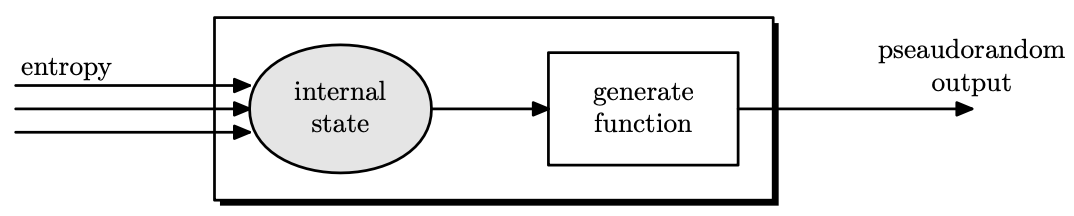
\includegraphics[width=0.7\linewidth]{figures/chapter3/fig14.png}
  \caption{一个随机数生成器}
  \label{fig:3-14}
\end{figure}

一个典型的例子是 Linux 操作系统中的 RNG,它被实现成一个名为 \texttt{/dev/random} 的设备。任何人都可以从该设备中读取到随机比特。你可以在 UNIX shell 中输出 \texttt{cat /dev/random} 来试着玩一玩这个工具,你将会看到一串无休止的、看起来很随机的字符。UNIX RNG 从一些硬件来源获得随机熵,包括:
\begin{itemize}
	\item 键盘事件:按键时间间隔能够提供随机熵;
	\item 鼠标事件:中断时间和鼠标位置都能够提供随机熵;
	\item 硬件中断:硬件中断的时间间隔也能提供较高质量的随机熵。
\end{itemize}
这些随机源能够产生连续的随机流,并会被定期异或到 RNG 的内部状态上。请注意,具体的键盘输入内容不会被用作熵的来源,通常使用的只是按键的时间,这是为了确保用户的输入内容不会通过 RNG 泄露给系统中的其他用户。

\begin{snote}[高熵的随机生成。]
上述熵源产生随机流的速度相对较慢。为了以更快的速度生成真随机比特,英特尔从 2012 年的 Ivy Bridge 处理器系列开始,增加了一个硬件随机数生成器。使用 \texttt{RdRand} 指令即可读取这个生成器的输出,它旨在提供一个快速且均匀的随机比特生成器。

为了减少生成器输出中的偏差,原始比特首先通过一个被称为``调节器"的函数,以确保在提供足够熵源作为输入时,输出是一个均匀分布的比特序列。我们在 \ref{sec:8-10} 节讨论密钥推导问题时会更详细地讨论这个问题。

\texttt{RdRand} 发生器不应该取代其他的熵源,比如上面描述的几个熵源;它只应该作为 RNG 的一个\emph{额外的}熵源来增强它们。这样一来,如果生成器有缺陷,就不会完全影响到加密应用。

英特尔的方法的一个困难是,随着时间的推移,被采样的硬件元素可能由于硬件故障而停止产生随机流。例如,被采样的比特可能总是 ``$0$",这会导致高度非随机的输出。为了防止这种情况的发生,RNG 的输出会被不断地用一套固定的统计方法来测试。如果任何一项测试报告为``非随机",发生器就会被认为有缺陷。
\end{snote}
\section{一个更广阔的视角:计算上不可区分性}

我们对伪随机数发生器 $G$ 的安全性的定义将下面这个直观的想法进行了形式化,即对手不应该能够有效区分 $G(s)$ 和 $r$,其中 $s$ 是一个随机选出的种子,而 $r$ 是输出空间中的一个随机元素。

这个想法可以很自然地推广到其他场合。假设 $P_0$ 和 $P_1$ 是有限集 $\mathcal{R}$ 上的两个概率分布。我们的目标是定义一个直观的概念,即对手无法有效地区分 $P_0$ 和 $P_1$。与之前一样,这通过设计一个攻击游戏来完成。对于 $b=0,1$,我们记 $x\overset{\rm R}\leftarrow P_b$ 为根据概率分布 $P_b$ 从集合 $\mathcal R$ 中随机选出一个值赋给 $x$。

\begin{game}[区分 $P_0$ 和 $P_1$]\label{game:3-3}
对于有限集 $\mathcal{R}$ 上的给定概率分布 $P_0$ 和 $P_1$ 以及一个给定对手 $\mathcal A$,我们定义两个实验:实验 $0$ 和实验 $1$。对于 $b=0,1$,我们定义:

\noindent\textbf{实验 $b$:}
\begin{itemize}
	\item 挑战者计算 $x\overset{\rm R}\leftarrow P_b$,并将 $x$ 发送给对手。
	\item 给定 $x$,对手计算并输出一个比特 $\hat b\in\{0,1\}$。
\end{itemize}

对于 $b=0,1$,令 $W_b$ 为对手 $\mathcal A$ 在实验 $b$ 中输出 $1$ 的事件。 我们定义 $\mathcal A$ 相对于 $P_0$ 和 $P_1$ 的\textbf{优势}为:
\[
\mathrm{Dist}\mathsf{adv}[\mathcal{A},P_0,P_1]:=\big\lvert\Pr[W_0]-\Pr[W_1]\big\rvert
\]
\end{game}

\begin{definition}[计算上不可区分性]\label{def:3-4}
如果 $\mathrm{Dist}\mathsf{adv}[\mathcal{A},P_0,P_1]$ 的值对任意有效对手 $\mathcal A$ 来说均可忽略不计,则称概率分布 $P_0$ 和 $P_1$ \textbf{在计算上不可区分 (computationally indistinguishable)}。
\end{definition}

利用该定义,我们可以更简单地重新表述安全 PRG 的定义:如果 $P_1$ 是 $\mathcal R$ 上的均匀分布,$P_0$ 是对 $r\in\mathcal R$ 的赋值的概率分布:
\[
P_0(r):=\frac{|\{s\in\mathcal{S}:G(s)=r\}|}{|\mathcal{S}|}
\]
当且仅当 $P_0$ 和 $P_1$ 在计算上不可区分时,定义在 $(\mathcal S,\mathcal R)$ 上的 PRG 是安全的。

与 \ref{subsec:2-2-5} 中讨论的相同,攻击游戏 \ref{game:3-3} 可以被改写为一个``比特猜测"游戏,其中挑战者不再有两个独立的实验,而是随机选择一个 $b\in\{0,1\}$,然后与对手 $\mathcal A$ 运行实验 $b$。在这个游戏中,我们将 $\mathcal A$ 的\emph{比特猜测优势}$\mathrm{Dist}\mathsf{adv}^*[\mathcal{A},P_0,P_1]$记为$|\Pr[\hat b=b]-{1}/{2}|$。那么 \ref{subsec:2-2-5} 中的推广结论(即式 \ref{eq:2-11})也适用于此:
\begin{equation}
{\rm Dist\mathsf{adv}}[\mathcal{A},P_0,P_1]=2\cdot\mathrm{Dist}\mathsf{adv}^*[\mathcal{A},P_0,P_1]
\end{equation}

通常情况下,为了证明两个分布在计算上是不可区分的,我们不得不做某些其他的计算上的假设。然而有时两个分布真的极其相似,以至于无论对手有多么强大的计算能力,都无法有效区分它们。为了准确表述这种``相似性"的概念,我们下面将引入一个有用的工具,称为\textbf{统计距离 (statistical distance)}:

\begin{definition}[统计距离]\label{def:3-5}
假设 $P_0$ 和 $P_1$ 是有限集 $\mathcal R$ 上的概率分布,那么它们的\textbf{统计距离}定义为:
\[
\Delta[P_0,P_1]:=\frac{1}{2}\sum_{r\in\mathcal{R}}\big\lvert P_0(r)-P_1(r)\big\rvert
\]
\end{definition}

\begin{example}\label{exmp:3-1}
假设 $P_0$ 是 $\{1,\dots,m\}$ 上的均匀分布,$P_1$ 是 $\{1,\dots,m-\delta\}$ 上的均匀分布,其中 $\delta\in\{0,\dots,m-1\}$。我们下面试着计算 $\Delta[P_0,P_1]$。我们固然可以直接使用统计距离的定义来计算 $\Delta[P_0,P_1]$;但是,不妨考虑下面这张关于 $P_0$ 和 $P_1$ 的图:

\begin{figure*}[h!]
  \centering
  

\tikzset{every picture/.style={line width=0.75pt}} %set default line width to 0.75pt        

\begin{tikzpicture}[x=0.75pt,y=0.75pt,yscale=-1,xscale=1]
%uncomment if require: \path (0,300); %set diagram left start at 0, and has height of 300

%Straight Lines [id:da44485393234819215] 
\draw    (70,140) -- (370,140) ;
%Straight Lines [id:da865188063783277] 
\draw    (70,50) -- (70,140) ;
%Straight Lines [id:da19158122915410059] 
\draw    (70,50) -- (280,50) ;
%Straight Lines [id:da38010593816585625] 
\draw    (280,50) -- (280,140) ;
%Straight Lines [id:da8880042968224386] 
\draw  [dash pattern={on 4.5pt off 4.5pt}]  (70,90) -- (370,90) ;
%Straight Lines [id:da40410564631236867] 
\draw    (370,90) -- (370,140) ;

% Text Node
\draw (175,70) node    {$A$};
% Text Node
\draw (175,115) node    {$B$};
% Text Node
\draw (325,115) node    {$C$};
% Text Node
\draw (70,150) node    {$0$};
% Text Node
\draw (280,150) node    {$m-\delta $};
% Text Node
\draw (370,150) node    {$m$};
% Text Node
\draw (58,90) node [anchor=east] [inner sep=0.75pt]    {$1/m$};
% Text Node
\draw (58,50) node [anchor=east] [inner sep=0.75pt]    {$1/( m-\delta )$};


\end{tikzpicture}
\end{figure*}

$P_0$ 和 $P_1$ 的统计距离就是图中区域 $A$ 和区域 $C$ 面积和的一半。此外,由于概率分布的总和为 $1$,我们必然有:
\[
\text{area of } B+ \text{area of } A= 1 = \text{area of } B+ \text{area of } C
\]
因此区域 $A$ 和区域 $C$ 的面积相等。所以:
\[
\Delta[P_0,P_1]=\text{area of } A = \text{area of } C ={\delta}/{m}
\]
\end{example}

下面的定理使我们能够在计算上不可区分性和统计距离这两个概念之间建立起联系。

\begin{theorem}\label{theo:3-10}
令 $P_0$ 和 $P_1$ 是有限集 $\mathcal R$ 上的两个概率分布,那么我们有:
\[
\max_{\mathcal{R}'\subseteq\mathcal{R}}|P_0[\mathcal{R}']-P_1[\mathcal{R}']|=\Delta[P_0,P_1]
\]
其中,最大值在 $\mathcal R$ 的所有子集 $\mathcal R'$ 上都能取得。
\end{theorem}

\begin{proof}
假设我们把 $\mathcal{R}$ 分成两个互不相干的子集:由使得 $P_0(r)<P_1(r)$ 的 $r\in\mathcal R$ 组成的集合 $\mathcal{R}_0$,以及由使得 $P_0(r)\geq P_1(r)$ 的 $r\in\mathcal R$ 组成的集合 $\mathcal{R}_1$。考虑下面的 $P_0$ 和 $P_1$ 分布的示意图,其中 $\mathcal{R}_0$ 的元素被放在 $\mathcal{R}_1$ 的元素的左边:

\begin{figure*}[h!]
  \centering
  

\tikzset{every picture/.style={line width=0.75pt}} %set default line width to 0.75pt        

\begin{tikzpicture}[x=0.75pt,y=0.75pt,yscale=-1,xscale=1]
%uncomment if require: \path (0,178); %set diagram left start at 0, and has height of 178

%Straight Lines [id:da36257954469734544] 
\draw    (70,140) -- (370,140) ;
%Straight Lines [id:da7236983033636388] 
\draw    (70,70) -- (70,140) ;
%Straight Lines [id:da6165923641727589] 
\draw    (370,70) -- (370,140) ;
%Curve Lines [id:da901864953155475] 
\draw    (70,70) .. controls (103,29.8) and (123.36,1.75) .. (147.8,1.8) .. controls (212.68,1.94) and (282.98,112.93) .. (325.4,113.8) .. controls (344.24,113.81) and (353.8,110.2) .. (370,100) ;
%Curve Lines [id:da2681996341594639] 
\draw  [dash pattern={on 4.5pt off 4.5pt}]  (70,110) .. controls (283.4,85.4) and (289.8,48.6) .. (321,49.8) .. controls (338.6,50.2) and (354.2,59.8) .. (370,70) ;
%Straight Lines [id:da020360043822280627] 
\draw    (73,160) -- (252,160) ;
\draw [shift={(255,160)}, rotate = 180] [fill={rgb, 255:red, 0; green, 0; blue, 0 }  ][line width=0.08]  [draw opacity=0] (7.14,-3.43) -- (0,0) -- (7.14,3.43) -- (4.74,0) -- cycle    ;
\draw [shift={(70,160)}, rotate = 0] [fill={rgb, 255:red, 0; green, 0; blue, 0 }  ][line width=0.08]  [draw opacity=0] (7.14,-3.43) -- (0,0) -- (7.14,3.43) -- (4.74,0) -- cycle    ;
%Straight Lines [id:da9288058437346971] 
\draw    (268,160) -- (367,160) ;
\draw [shift={(370,160)}, rotate = 180] [fill={rgb, 255:red, 0; green, 0; blue, 0 }  ][line width=0.08]  [draw opacity=0] (7.14,-3.43) -- (0,0) -- (7.14,3.43) -- (4.74,0) -- cycle    ;
\draw [shift={(265,160)}, rotate = 0] [fill={rgb, 255:red, 0; green, 0; blue, 0 }  ][line width=0.08]  [draw opacity=0] (7.14,-3.43) -- (0,0) -- (7.14,3.43) -- (4.74,0) -- cycle    ;
%Shape: Rectangle [id:dp8000548924440445] 
\draw  [draw opacity=0][fill={rgb, 255:red, 255; green, 255; blue, 255 }  ,fill opacity=1 ] (147.5,150) -- (177.5,150) -- (177.5,170) -- (147.5,170) -- cycle ;
%Shape: Rectangle [id:dp3066289561795965] 
\draw  [draw opacity=0][fill={rgb, 255:red, 255; green, 255; blue, 255 }  ,fill opacity=1 ] (302.5,150) -- (332.5,150) -- (332.5,170) -- (302.5,170) -- cycle ;

% Text Node
\draw (151,54.8) node    {$A$};
% Text Node
\draw (226.6,109.4) node    {$B$};
% Text Node
\draw (325.8,83.8) node    {$C$};
% Text Node
\draw (58,70) node [anchor=east] [inner sep=0.75pt]    {$P_{1}$};
% Text Node
\draw (58,110) node [anchor=east] [inner sep=0.75pt]    {$P_{0}$};
% Text Node
\draw (162.5,160) node  [color={rgb, 255:red, 0; green, 0; blue, 0 }  ,opacity=1 ]  {$\mathcal{R}_{0}$};
% Text Node
\draw (317.5,160) node  [color={rgb, 255:red, 0; green, 0; blue, 0 }  ,opacity=1 ]  {$\mathcal{R}_{1}$};


\end{tikzpicture}
\end{figure*}

现在,与例 \ref{exmp:3-1} 中一样,我们有:
\[
\Delta[P_0,P_1]=\text{area of } A = \text{area of } C
\]
注意到,对于 $\mathcal{R}$ 的每个子集 $\mathcal{R}'$,我们都有:
\[
P_0[\mathcal{R}']-P_1[\mathcal{R}']=\text{area of } C' - \text{area of } A'
\]
其中 $C'$ 指位于 $\mathcal{R}'$ 上的 $C$ 的子区域,$A'$ 指位于 $\mathcal{R}'$ 上的 $A$ 的子区域。由此可知,当 $\mathcal{R}'=\mathcal{R}_0$ 或 $\mathcal{R}'=\mathcal{R}_1$ 时,$|P_0[\mathcal{R}']-P_1[\mathcal{R}']|$ 取得最大值,此时最大值就等于 $\Delta[P_0,P_1]$。
\end{proof}

与计算上不可分性的联系如下:

\begin{theorem}\label{theo:3-11}
假设 $P_0$ 和 $P_1$ 是有限集 $\mathcal{R}$ 上的概率分布,那么对于任意对手 $\mathcal A$,我们都有:
\[
{\rm Dist\mathsf{adv}}[\mathcal{A},P_0,P_1]\leq\Delta[P_0,P_1]
\]
\end{theorem}

\begin{proof}
考虑一个如攻击游戏 \ref{game:3-3} 中那样试图区分 $P_0$ 和 $P_1$ 的对手 $\mathcal A$。

首先,我们考虑 $\mathcal A$ 是确定性算法的情况。在这种情况下,$\mathcal A$ 的输出是一个 $r\in\mathcal{R}$ 的函数 $f(r)$,它是由挑战者发送给 $\mathcal A$ 的。令 $\mathcal{R}':=\{r\in\mathcal{R}:f(r)=1\}$。如果 $W_0$ 和 $W_1$ 是攻击游戏 \ref{game:3-3} 中定义的两个事件,那么对于 $b=0,1$,我们有:
\[
\Pr[W_b]=P_b[\mathcal{R}']
\]
根据定理 \ref{theo:3-10},我们有:
\[
{\rm Dist\mathsf{adv}}[\mathcal{A},P_0,P_1]=|P_0[\mathcal{R}']-P_1[\mathcal{R}']|\leq\Delta[P_0, P_1]
\]

我们下面考虑 $\mathcal A$ 是概率性算法的情况。我们可以认为 $\mathcal A$ 接受一个辅助输入 $t$ ,代表它的随机选择。我们认为 $t$ 是从某个有限集 $\mathcal{T}$ 中均匀随机选出的。因此,$\mathcal A$ 的输出是挑战者交给它的值 $r\in\mathcal{R}$ 和代表其随机选择的值 $t\in\mathcal{T}$ 的函数 $g(r,t)$。对于一个给定的 $t\in\mathcal{T}$,令 $\mathcal{R}_t':=\{r\in\mathcal{R}:g(r,t)=1\}$。然后,对 $t$ 的随机选择进行平均化,我们有:
\[
\Pr[W_b]=\frac{1}{|\mathcal{T}|}\sum_{t\in\mathcal{T}}P_b[\mathcal{R}_t']
\]
由此可得:
\[
\begin{aligned}
{\rm Dist\mathsf{adv}}[\mathcal{A},P_0,P_1]
&=|P_0[\mathcal{R}']-P_1[\mathcal{R}']|\\
&=\frac{1}{|\mathcal{T}|}\bigg\lvert\sum_{t\in\mathcal{T}}(P_0[\mathcal{R}_t']-P_1[\mathcal{R}_t'])\bigg\rvert\\
&\leq\frac{1}{|\mathcal{T}|}\sum_{t\in\mathcal{T}}|P_0[\mathcal{R}_t']-P_1[\mathcal{R}_t']|\\
&\leq\frac{1}{|\mathcal{T}|}\sum_{t\in\mathcal{T}}\Delta[P_0,P_1]\\
&=\Delta[P_0,P_1]\qedhere
\end{aligned}
\]
\end{proof}

作为该定理的一个结论,我们可以看到,如果 $\Delta[P_0,P_1]$ 可忽略不计,那么 $P_0$ 和 $P_1$ 是计算上不可区分的。

\vspace{5pt}

我们还可以将两个随机变量之间的统计距离定义为它们相应分布之间的统计距离。也就是说,如果 $\mathsf{X}$ 和 $\mathsf{Y}$ 是在一个有限集 $\mathcal{R}$ 中取值的随机变量,那么它们的\textbf{统计距离}是:
\[
\Delta[\mathsf{X},\mathsf{Y}]
:=
\frac{1}{2}
\sum_{r\in\mathcal{R}}
|\Pr[\mathsf{X}=r]-Pr[\mathsf{Y}=r]|
\]
在这种情况下,定理 \ref{theo:3-10} 表明:
\[
\max_{\mathcal{R}'\subseteq\mathcal{R}}
|\Pr[\mathsf{X}\in\mathcal{R}']-\Pr[\mathsf{Y}\in\mathcal{R}']|=\Delta[\mathsf{X},\mathsf{Y}]
\]
其中,最大值在 $\mathcal R$ 的所有子集 $\mathcal R'$ 上都能取得。

类似地,我们还可以对随机变量而非分布来定义区分优势。使用随机变量的好处是,我们可以更方便地处理彼此相关的分布,正如下面的定理所例证的那样。

\begin{theorem}\label{theo:3-12}
如果 $\mathcal{S}$ 和 $\mathcal{T}$ 是有限集,$\mathsf{X}$ 和 $\mathsf{Y}$ 是在 $\mathcal{S}$ 上取值的随机变量,并且 $f:\mathcal{S}\to\mathcal{T}$ 是一个函数,那么 $\Delta[f(\mathsf{X}),f(\mathsf{Y})]\leq\Delta[\mathsf{X},\mathsf{Y}]$。
\end{theorem}

\begin{proof}
对于某个 $\mathcal{T}'\subseteq\mathcal{T}$,我们有:
\[
\begin{aligned}
\Delta[f(\mathsf{X}),f(\mathsf{Y})]
&=|\Pr[f(\mathsf{X})\in\mathcal{T}']-\Pr[f(\mathsf{Y})\in\mathcal{T}']|\quad\text{\emph{(根据定理} \ref{theo:3-10}\emph{\,)}}\\
&=|\Pr[\mathsf{X}\in f^{-1}(\mathcal{T}')]-\Pr[\mathsf{Y}\in f^{-1}(\mathcal{T}')]|\\
&\leq\Delta[\mathsf{X},\mathsf{Y}]\quad\text{\emph{(根据定理} \ref{theo:3-10}\emph{\,)}}\qedhere
\end{aligned}
\]
\end{proof}

\begin{example}\label{exmp:3-2}
令 $\mathsf{X}$ 均匀分布在集合 $\{0,\dots,m-1\}$ 上,$\mathsf{Y}$ 均匀分布在集合 $\{0,\dots,N-1\}$ 上,且 $N\geq m$。令 $f(t):=t\;\mathrm{mod}\;m$。我们想计算 $\mathsf{X}$ 和 $f(\mathsf{Y})$ 之间的统计距离的上界。我们可以这样做。令 $N=qm-r$,其中 $0\leq r<m$,因此 $q=\lceil{N}/{m}\rceil$。同时,令 $\mathsf{Z}$ 均匀分布在集合 $\{0,\dots,qm-1\}$ 上。那么 $f(\mathsf{Z})$ 就均匀分布在集合 $\{0,\dots,m-1\}$ 上,这是因为 $\{0,\dots,m-1\}$ 中的每个元素在函数 $f$ 下都有相同个数的原像(即$q$个),这些原像都落在集合 $\{0,\dots,qm-1\}$ 中。由于统计距离只取决于随机变量的分布,根据定理 \ref{theo:3-12},我们有:
\[
\Delta[\mathsf{X},f(\mathsf{Y})]=\Delta[f(\mathsf{Z}),f(\mathsf{Y})]\leq\Delta[\mathsf{Z},\mathsf{Y}]
\]
正如我们在例 \ref{exmp:3-1} 中所看到的:
\[
\Delta[\mathsf{Z},\mathsf{Y}]=\frac{r}{qm}<\frac{1}{q}\leq\frac{m}{N}
\]
因此有:
\[
\Delta[\mathsf{X},f(\mathsf{Y})]<\frac{m}{N}
\]
\end{example}

\begin{example}
现在我们想要生成一个给定区间 $\{0,\dots,m-1\}$ 上的伪随机数。假设我们有一个PRG $G$,它可以输出 $L$ 比特的序列。当然,一个 $L$ 比特的序列可以被看作是 $\{0,\dots,N-1\}$ 中的一个数,其中 $N:=2^L$。让我们假设 $N\geq m$。

为了生成一个区间 $\{0,\dots,m-1\}$ 上的伪随机数,我们可以把 $G$ 的输出看作是 $\{0,\dots,N-1\}$ 中的一个数,并将其模 $m$ 后输出。我们下面将表明,只要 $G$ 是安全的,且 ${m}/{N}$ 可忽略不计,上述方法所产生的数和从区间 $\{0,\dots,m-1\}$ 中随机挑选的真随机数在计算上不可区分。

为此,令 $P_0$ 为 $G$ 输出并模 $m$ 后的分布,$P_1$ 为 $\{0,\dots,m-1\}$ 上的均匀分布,令 $\mathcal A$ 是一个试图区分 $P_0$ 和 $P_1$ 的对手,就像在攻击游戏 \ref{game:3-3} 中的那样。

令游戏 $0$ 为攻击游戏 \ref{game:3-3} 中的实验 $0$,在这个实验中,$\mathcal A$ 被赋予了一个按照 $P_0$ 分布的随机样本,记 $W_0$ 是 $\mathcal A$ 在游戏 $0$ 中输出 $1$ 的事件。

现在,定义游戏 $1$ 与游戏 $0$ 基本相同,只是我们用一个从区间 $\{0,\dots,N-1\}$ 中随机选出的真随机数代替 $G$ 的输出。记 $W_1$ 为 $\mathcal A$ 在游戏 $1$ 中输出 $1$ 的事件。我们很容易构建出一个有效对手 $\mathcal{B}$,它可以像攻击游戏 \ref{game:3-1} 中那样攻击 $G$,并使得:
\[
{\rm PRG\mathsf{adv}}[\mathcal{B},G]=|{\rm Pr}[W_0]-{\rm Pr}[W_1]|
\]
思路是 $\mathcal{B}$ 获取到它的挑战值并模 $m$,然后将这个值交给 $\mathcal A$,然后原样输出 $\mathcal A$ 输出的任何东西。

最后,我们定义游戏 $2$ 为攻击游戏 \ref{game:3-3} 中的实验 $1$,在这个实验中,$\mathcal A$ 被赋予了一个按照 $P_1$ 分布的随机样本,也就是 $\{0,\dots,m-1\}$ 上的均匀分布。记 $W_2$ 为 $\mathcal A$ 在游戏 $2$ 中输出 $1$ 的事件。如果 $P$ 是游戏 $1$ 中交给 $\mathcal A$ 的值的分布,那么根据定理 \ref	{theo:3-11},我们就有 $|\Pr[W_1]-\Pr[W_2]|\leq\Delta[P,P_1]$;此外,根据例 \ref{exmp:3-2},我们还有 $\Delta[P,P_1]\leq{m}/{N}$。

将以上结论综合起来,可以得到:
\[
\begin{aligned}
{\rm Dist\mathsf{adv}}[\mathcal{A},P_0,P_1]
&=|\Pr[W_0]-\Pr[W_2]|\leq|\Pr[W_0]-\Pr[W_1]|+|\Pr[W_1]-\Pr[W_2]|\\
&\leq{\rm PRG\mathsf{adv}}[\mathcal{B},G]+\frac{m}{N}
\end{aligned}
\]
而根据假设,该值可忽略不计。
\end{example}

\subsection{数学细节}

和之前一样,我们下面会详述相关的数学细节,以便从渐进复杂性理论的角度解释本节的定义和结论。

在定义计算上不可区分性(定义 \ref{def:3-4})时,我们应该考虑两个概率分布族 $P_0=\{P_{0,\lambda}\}_{\lambda}$ 和 $P_1=\{P_{1,\lambda}\}_{\lambda}$,它们都由安全参数 $\lambda$ 索引。对于每个 $\lambda$,分布 $P_{0,\lambda}$ 和 $P_{1,\lambda}$ 都应该在有限比特序列集合 $\mathcal{R}_\lambda$ 中取值,其中 $\mathcal{R}_\lambda$ 中的序列长度以 $\lambda$ 的多项式为界。 在攻击游戏 \ref{game:3-3} 中,安全参数 $\lambda$ 是挑战者和对手的输入,而在实验 $b$ 中,挑战者产生一个根据 $P_{b,\lambda}$ 分布的样本。优势应当被正确地表记为 ${\rm Dist\mathsf{adv}}[\mathcal{A},P_0,P_1](\lambda)$,它是 $\lambda$ 的一个函数,而计算上不可区分性意味着该函数可以忽略不计。

在某些情况下,引入一个概率生成的系统参数可能是很自然的;然而,从技术角度来看,这不是必要的,因为这样的系统参数可以被纳入到分布 $P_{0,\lambda}$ 和 $P_{1,\lambda}$ 中。我们还可以要求 $P_{0,\lambda}$ 和 $P_{1,\lambda}$ 是可有效采样的;然而,为了保持定义的简单性,我们不会强制要求这样做。

统计距离的定义(定义 \ref{def:3-5})从非渐进的角度来看是完全合理的,不需要任何修改或阐述。如前所述,定理 \ref{theo:3-10} 对特定的分布 $P_0$ 和 $P_1$ 成立。定理 \ref{theo:3-11} 可以渐进地看作是说,对于所有分布族 $P_0=\{P_{0,\lambda}\}_{\lambda}$ 和 $P_1=\{P_{1,\lambda}\}_{\lambda}$,对于任意对手(甚至是计算上无界的对手),以及对于所有 $\lambda$,我们都有:
\[
{\rm Dist\mathsf{adv}}[\mathcal{A},P_0,P_1](\lambda)\leq\Delta[P_{0,\lambda},P_{1,\lambda}]
\]
\section{一个有趣的应用:抛掷硬币与比特承诺}\label{sec:3-12}

Alice 和 Bob 要出去约会了。Alice 想看某一部电影,而 Bob 想看另一部。他们决定抛一枚硬币来随机选择电影。如果抛硬币的结果是正面,他们就去看 Alice 选择的电影,否则就去看 Bob 选择的电影。当 Alice 和 Bob 离得很近的时候,这很容易操作:他们中的一个人,比如说 Bob,抛出一枚硬币,他们都能验证这个结果。但当他们相距甚远,并且在电话中交谈时,这就比较难了。Bob 可以在他那边掷硬币,然后告诉 Alice 结果,但是 Alice 却没有理由相信这个结果。Bob 可以简单地声称抛硬币的结果是反面,而 Alice 则没有办法证实这一点。这不是一个开始约会的好方法。

解决这个问题的一个简单方法是利用一种叫做\textbf{比特承诺(bit commitment)}的密码学原语。它能够让 Bob 承诺一个他选择的比特 $b\in\{0,1\}$。稍后,Bob 可以打开承诺,让 Alice 相信 $b$ 是 Bob 所承诺的值。承诺一个比特 $b$ 会产生一个\textbf{承诺序列(commitment string)} $c$,它会被 Bob 发送给 Alice;还会产生一个\textbf{打开序列(opening string)},它在之后会被 Bob 用于打开承诺。如果一个承诺方案满足以下两个特性,它就是安全的:
\begin{itemize}
	\item \textbf{隐藏(hiding)}:承诺序列 $c$ 不会透露关于承诺比特 $b$ 的任何信息。更确切地说,承诺比特为 $0$ 时 $c$ 的分布与承诺比特为 $1$ 时 $c$ 的分布是不可区分的。在我们提出的比特承诺方案中,隐藏属性取决于特定的 PRG $G$ 的安全性。
	\item \textbf{绑定(binding)}:令 $c$ 是 Bob 输出的承诺序列。如果 Bob 可以将该承诺打开为某个 $b\in\{0,1\}$,他就不能将其打开为 $\bar{b}$。这就保证了,一旦 Bob 承诺了一个比特 $b$,他就只可以把它打开为 $b$,而不能是其他的值。在我们提出的承诺方案中,绑定属性无条件成立。
\end{itemize}

\begin{snote}[抛掷硬币。]
使用一个承诺方案,Alice 和 Bob 就可以生成一个随机比特 $b\in\{0,1\}$,这样,假设协议成功终止,任何一方都不能使结果朝着自己的方向偏移。这样的协议被称为\textbf{抛掷硬币协议(coin flipping protocols)}。结果比特 $b$ 将决定他们去看什么电影。

Alice 和 Bob 使用下面这个简单的抛掷硬币协议:

\vspace*{10pt}

\hspace*{5pt} 步骤 1:Bob 随机选择一个比特 $b_0\overset{\rm R}\leftarrow\{0,1\}$。\\
\hspace*{66pt} Alice 和 Bob 执行承诺协议。\\
\hspace*{66pt} 通过该协议,Alice 获得对 $b_0$ 的承诺 $c$,Bob 获得一个打开序列 $s$。\\
\hspace*{26pt} 步骤 2:Alice 随机选择一个比特 $b_1\overset{\rm R}\leftarrow\{0,1\}$,并将其明文发送给 Bob。\\
\hspace*{26pt} 步骤 3:Bob 通过向 Alice 揭露 $b_0$ 和 $s$ 来打开承诺。\\
\hspace*{66pt} Alice 验证 $c$ 是否是对 $b_0$ 的承诺,如果验证失败则终止。

\vspace*{5pt}

\hspace*{5pt} 输出:结果比特 $b:=b_0\oplus b_1$。

\vspace*{10pt}

\noindent
我们声称,如果协议成功终止,并且一方诚实地遵守协议,那么另一方就不能使结果朝它的倾向偏移。根据隐藏属性,Alice 在步骤 $1$ 结束时不会得到任何关于 $b_0$ 的信息,因此她对 $b_1$ 的选择与 $b_0$ 的值无关。根据绑定属性,Bob 只能在步骤 $3$ 中对他在步骤 $1$ 中选择的 $b_0$ 打开承诺 $c$。而由于他在 Alice 选择 $b_1$ 之前就选择了 $b_0$,所以 Bob 对 $b_0$ 的选择与 $b_1$ 无关。我们可以得出结论,输出比特 $b$ 是两个独立比特的异或。因此,如果一方诚实地遵守协议,另一方就不可能使产生的比特有所偏向。

这个协议的一个问题是,Bob 在步骤 $2$ 结束时,在 Alice 获取比特之前就知道了生成的比特。原则上,如果结果不是 Bob 想要的,他也可以在步骤 $2$ 结束时中止协议,并试图重新启动协议,并且期待下一次运行能得到他想要的结果。更复杂的抛掷硬币协议能够避免这个问题,但代价是需要更多回合的交互(比如,参见 \cite{moran2009optimally})。
\end{snote}

\begin{snote}[来自安全PRG的比特承诺。]
剩下的工作就是构建一个让 Bob 承诺他的比特 $b_0\in\{0,1\}$ 的安全比特承诺方案。我们使用 Naor 提出的一个优雅的构造来完成这个工作 \cite{naor1989bit}。

令 $G:\mathcal{S}\to\mathcal{R}$ 是一个安全的 PRG,其中 $|\mathcal{R}|\geq|\mathcal{S}|^3$,$\mathcal{R}=\{0,1\}^n$,$n$ 是某个正整数。为了承诺比特 $b_0$,Alice 和 Bob 参与以下协议:

\vspace*{5pt}

\hspace*{5pt} Bob 承诺比特 $b_0\in\{0,1\}$:\\
\hspace*{50pt} 步骤 1:Alice 随机选择一个 $r\in\mathcal{R}$,并将 $r$ 发送给 Bob。\\
\hspace*{50pt} 步骤 2:Bob 随机选择一个 $s\in\mathcal{S}$ 并计算 $c\leftarrow\mathrm{com}(s,r,b_0)$\\
\hspace*{90pt} 其中 $\mathrm{com}(s,r,b_0)$ 是以下函数:\\
\[
c=\mathrm{com}(s,r,b_0):=
\left\{
\begin{array}{ll}
G(s), & b_0=0\\
G(s)\oplus r, & b_0=1
\end{array}	
\right.
\]

\hspace*{5pt} Bob 输出 $c$ 作为承诺序列,并将 $s$ 作为打开序列。

\vspace*{5pt}

\noindent
当到了打开承诺的时候,Bob 将 $(b_0,s)$ 发送给 Alice。如果 $c=\mathrm{com}(s,r,b_0)$ 成立,Alice 就接受打开值,否则就拒绝它。

隐藏属性直接来自于 PRG 的安全性:因为输出 $G(s)$ 与 $\mathcal{R}$ 上的均匀随机序列在计算上是不可区分的,所以 $G(s)\oplus r$ 与 $\mathcal{R}$ 上的均匀随机序列在计算上也是不可区分的。因此,无论是 $b_0=0$ 还是 $b_0=1$,承诺序列 $c$ 与 $\mathcal{R}$ 上的均匀序列在计算上都是不可区分的,正如所要求的那样。

只要 $1/|\mathcal{S}|$ 可忽略不计,绑定属性就无条件成立。Bob 可以将一个承诺 $c\in\mathcal{R}$ 打开为 $0$ 和 $1$ 的唯一办法,就是找到两个种子 $s_0,s_1\in\mathcal{S}$ 满足 $c=G(s_0)=G(s_1)\oplus r$,这意味着 $G(s_0)\oplus G(s_1)=r$。如果存在种子 $s_0,s_1\in\mathcal{S}$ 满足 $G(s_0)\oplus G(s_1)=r$,我们就称这样的 $r\in\mathcal{R}$ 是``坏的"。种子对 $(s_0,s_1)$ 的数量是 $|\mathcal{S}|^2$,因此坏的 $r$ 的数量最多也是 $|\mathcal{S}|^2$。由此可见,Alice 选到坏的 $r$ 的概率最多为 $|\mathcal{S}|^2/|\mathcal{R}| < |\mathcal{S}|^2/|\mathcal{S}|^3 = 1/|\mathcal{S}|$,该值可忽略不计。因此,Bob 能把承诺 $c$ 打开为 $0$ 和 $1$ 的概率是可忽略不计的。
\end{snote}

这样,我们就完成了对比特承诺方案的介绍。我们将在 \ref{sec:8-12} 节看到一个更有效的承诺方案以及更多与承诺有关的应用,但在那之前,我们还需要引入更多的密码学工具。
\section{笔记}\label{sec:3-13}

对文献的引用有待补充。

\section{练习}
